\RequirePackage{amsmath} 

\documentclass[graybox,envcountsect]{svmono}

\usepackage{amsmath}
\usepackage{float}
\usepackage{amssymb}
\usepackage{amstext}
\usepackage{mathtools}
\usepackage{anyfontsize}
\usepackage{xcolor} 
\usepackage{centernot}
\usepackage{listings}
\usepackage{multicol}
\usepackage{mathptmx}
\usepackage{newtxtext,newtxmath}
\usepackage{datetime}
\usepackage{stmaryrd}
\usepackage{tikz-cd}
\usepackage{fancyhdr}
\usepackage[final]{hyperref} 


\usepackage{helvet}
\usepackage{courier}
\usepackage{type1cm}         
\usepackage{makeidx}        
\usepackage{graphicx}        
\usepackage{multicol}        
\usepackage{hyperref} 
%\usepackage{tikz-cd}
\usepackage{colortbl}
\usepackage{chngcntr}
\usepackage{quiver}

% Table of contents for lectures and topics
\makeatletter
\newcommand\listtopicsname{List of topics}
\newcommand\listoftopics{
    \chapter*{\listtopicsname}\@starttoc{top}}
\makeatother

\makeatletter
\newcommand\listlecturesname{Contents}
\newcommand\listoflectures{
    \chapter*{\listlecturesname}\@starttoc{lec}}
\makeatother

\newcommand{\lecture}[1]{
    \chapter{#1}
    \addcontentsline{lec}{chapter}{Lecture \thechapter}
}

\newcommand{\topic}[1]{
    \section{#1}
    \addcontentsline{top}{chapter}{\S\thesection\quad #1}
}


%\usepackage[small,bf]{caption}

\usepackage{tikz}
\usetikzlibrary{braids}
	
\usepackage[bottom]{footmisc}

% for QED
\let\proof\relax\let\endproof\relax
\let\openbox\relax
\usepackage{amsthm}

\overfullrule=1mm

%%% for Spanish
% \def\abstractname{Resumen}%
% \def\ackname{Agradecimientos}%
% \def\andname{y}%
% \def\bibname{Referencias}%
% \def\lastandname{, y}%
% \def\appendixname{Apéndice}%
\def\chaptername{Lecture}%
% \def\claimname{Afirmación}%
% \def\conjecturename{Conjetura}%
% \def\contentsname{Contenidos}%
% \def\corollaryname{Corolario}%
% \def\definitionname{Definici\'on}%
% \def\emailname{e-mail}%
% \def\examplename{Ejemplo}%
\def\examplesname{Examples}%
% \def\exercisename{Ejercicio}%
\def\figurename{Figure}%
% \def\forewordname{Foreword}%
% \def\keywordname{{\bf Palabras clave:}}%
% \def\indexname{Índice}%
% \def\lemmaname{Lema}%
% \def\listfigurename{Figuras}%
% \def\listtablename{Tablas}%
% \def\notename{Nota}%
% \def\partname{Parte}%
% \def\prefacename{Prefacio}%
\def\problemname{Open problem}%
% \def\proofname{Demostración}%
% \def\propertyname{Propiedad}%
% \def\propositionname{Proposici\'on}%
% \def\questionname{Pregunta}%
% \def\refname{Referencias}%
% \def\remarkname{Observación}%
% \def\seename{see}%
% \def\solutionname{Solución}%
% \def\tablename{Tabla}%
% \def\theoremname{Teorema}
\def\notationname{Notation}
\def\stepsname{Algorithm}
% \def\conventionname{Convención}

% change numbers 
\let\remark\relax
\let\theorem\relax
\let\lemma\relax
\let\definition\relax
\let\proposition\relax
\let\corollary\relax
\let\exercise\relax
\let\example\relax
\let\conjecture\relax

% Numerar con sección y no resetear al cambiar de capítulo
\counterwithout{section}{chapter}
\counterwithout{theorem}{chapter}
\spnewtheorem{theorem}{\theoremname}[section]{\bfseries}{\itshape}

\renewcommand\thetheorem{\thesection.\arabic{theorem}}
\spnewtheorem{lemma}[theorem]{\lemmaname}{\bfseries}{\itshape}
\spnewtheorem{definition}[theorem]{\definitionname}{\bfseries}{\upshape}
\spnewtheorem{proposition}[theorem]{\propositionname}{\bfseries}{\itshape}
\spnewtheorem{corollary}[theorem]{\corollaryname}{\bfseries}{\itshape}
\spnewtheorem{exercise}[theorem]{\exercisename}{\bfseries}{\upshape}
\spnewtheorem{example}[theorem]{\examplename}{\bfseries}{\upshape}
\spnewtheorem{examples}[theorem]{\examplesname}{\bfseries}{\upshape}
\spnewtheorem{remark}[theorem]{\remarkname}{}{\upshape}
\spnewtheorem{conjecture}[theorem]{\conjecturename}{\bfseries}{\upshape}
\spnewtheorem{notation}[theorem]{\notationname}{\bfseries}{\upshape}
\spnewtheorem{steps}[theorem]{\stepsname}{\bfseries}{\upshape}
\spnewtheorem{convention}[theorem]{\conventionname}{\bfseries}{\upshape}
\spnewtheorem{openproblem}[theorem]{\problemname}{\bfseries}{\upshape}


% Numerar con sección y no resetear al cambiar de capítulo
\counterwithout{section}{chapter}

% No sections in TOC
\setcounter{secnumdepth}{1}
\setcounter{tocdepth}{0}

 \usepackage{titlesec}
 \titleformat{\section}
   {\secsize\secstyle}{\S\thesection.}{1em}{}

% para enumerar
\renewcommand{\labelenumi}{\textbf{\arabic{enumi})}}

\makeindex             

\renewcommand{\I}{\operatorname{I}}
\newcommand{\II}{\operatorname{II}}

\newcommand{\GAP}{\textsf{GAP}}
\newcommand{\FK}{\mathcal{E}}
\newcommand{\ad}[1]{\operatorname{ad}\,#1}

%\newcommand{\N}{\mathbb{N}}
\newcommand{\Q}{\mathbb{Q}}
\newcommand{\Z}{\mathbb{Z}}
\newcommand{\F}{\mathbb{F}}
\newcommand{\R}{\mathbb{R}}
\newcommand{\C}{\mathbb{C}}
\renewcommand{\H}{\mathbb{H}}
\newcommand{\A}{\mathbb{A}}
\newcommand{\K}{\mathbb{K}}
\newcommand{\T}{\mathbb{T}}
\renewcommand{\D}{\mathbb{D}}
\newcommand{\B}{\mathbb{B}}
\newcommand{\Fun}{\operatorname{Fun}}
\newcommand{\mpl}{\operatorname{mpl}}
\newcommand{\cL}{\mathcal{L}}
\newcommand{\cE}{\mathcal{E}}
\newcommand{\cH}{\mathcal{H}}

\newcommand{\GF}{\mathsf{GF}}
\newcommand{\MAX}{\operatorname{MAX}}
\newcommand{\MIN}{\operatorname{MIN}}
\newcommand{\cf}{\operatorname{cf}}
\newcommand{\cl}{\operatorname{cl}}
\newcommand{\cd}{\operatorname{cd}}
\newcommand{\bL}{\mathbf{L}}
\newcommand{\bP}{\mathbf{P}}

\newcommand{\Nil}{\operatorname{Nil}}
\newcommand{\rad}{\operatorname{rad}}
\newcommand{\rank}{\operatorname{rank}}
\newcommand{\cp}{\operatorname{cp}}
\newcommand{\Aff}{\mathrm{Aff}}
\newcommand{\Ann}{\operatorname{Ann}}
\newcommand{\Der}{\operatorname{Der}}
\newcommand{\Core}{\operatorname{Core}}
\newcommand{\Soc}{\operatorname{Soc}}
\newcommand{\Fix}{\operatorname{Fix}}
\newcommand{\Rad}{\mathrm{rad}}
\newcommand{\Inn}{\mathrm{Inn}}
\newcommand{\dist}{\mathrm{dist}}
\newcommand{\Out}{\mathrm{Out}}
\newcommand{\Ext}{\mathrm{Ext}}
\newcommand{\Img}{\mathrm{im}}
\newcommand{\Hol}{\operatorname{Hol}}
\newcommand{\Hom}{\operatorname{Hom}}
\newcommand{\Alg}{\operatorname{Alg}}
\newcommand{\Bil}{\operatorname{Bil}}
\newcommand{\op}{\operatorname{op}}
\newcommand{\gr}{\operatorname{gr}}
\newcommand{\Syl}{\mathrm{Syl}}
\newcommand{\id}{\operatorname{id}}
\newcommand{\Aut}{\operatorname{Aut}}
\newcommand{\End}{\operatorname{End}}
\newcommand{\Irr}{\operatorname{Irr}}
\newcommand{\Char}{\operatorname{Char}}
\newcommand{\Alt}{\mathbb{A}}
\newcommand{\Sym}{\mathbb{S}}
\newcommand{\lcm}{\mathrm{mcm}}
\newcommand{\diag}{\operatorname{diag}}
\newcommand{\spec}{\operatorname{Spec}}
\newcommand{\supp}{\operatorname{supp}}
\newcommand{\trace}{\operatorname{trace}}
\newcommand{\sgn}{\operatorname{sign}}
\newcommand{\ch}{\operatorname{char}}

\newcommand{\Res}{\operatorname{Res}}
\newcommand{\Ind}{\operatorname{Ind}}


\newcommand{\fg}{\mathfrak{g}}
\newcommand{\gl}{\mathfrak{gl}}
\renewcommand{\sl}{\mathfrak{sl}}
\newcommand{\fh}{\mathfrak{h}}


\newcommand{\inner}{\operatorname{inn}}
\newcommand{\ext}{\operatorname{ext}}
\newcommand{\im}{\operatorname{im}}
\newcommand{\Ret}{\operatorname{Ret}}

\newcommand{\GL}{\mathbf{GL}}
\newcommand{\SL}{\mathbf{SL}}
\newcommand{\PSL}{\mathbf{PSL}}
\newcommand{\PGL}{\mathbf{PGL}}

\newcommand{\legendre}[2]{\left(\frac{#1}{#2}\right)}

%\newcommand{\char}{\operatorname{char}}

% multiset
\def\multiset#1#2{\ensuremath{\left(\kern-.3em\left(\genfrac{}{}{0pt}{}{#1}{#2}\right)\kern-.3em\right)}}

% column vector
\newcount\colveccount
\newcommand*\colvec[1]{
\global\colveccount#1
\begin{pmatrix}
	\colvecnext
	}
	\def\colvecnext#1{
	#1
	\global\advance\colveccount-1
	\ifnum\colveccount>0
	\\
	\expandafter\colvecnext
	\else
\end{pmatrix}
\fi
}


% numero como secciones
\renewcommand{\thesection}{\arabic{section}}
%\renewcommand{\thesubsection}{\Alph{section}}

% To remove Springer from the title page
\usepackage{etoolbox}
\makeatletter
\patchcmd{\@maketitle}{{\Large Springer\par}}{}{}{}
\def\ps@bchap{%
  \let\@oddhead\@empty\let\@evenhead\@empty
  \def\@oddfoot{\reset@font\small\hfil\thepage\hfil}%
  \let\@evenfoot\@oddfoot
}

% Heading 
\def\ps@headings{%
  \let\@mkboth\markboth
  \def\@oddfoot{\reset@font\small\hfil\thepage\hfil}%
  \let\@evenfoot\@oddfoot
  \def\@evenhead{\runheadsize\runheadstyle\hfil\leftmark}%
  \def\@oddhead{\runheadsize\runheadstyle\rightmark\hfil}%
  \def\chaptermark##1{%
    \markboth{%
      {\if@chapnum Lecture \thechapter\thechapterend\fi ##1}%
    }{%
      {\if@chapnum Lecture \thechapter\thechapterend\fi ##1}}%
    }%
    \def\sectionmark##1{\markright{{\ifnum\c@secnumdepth>\z@
     \S\thesection\seccounterend\hskip\betweenumberspace\fi ##1}}}
}
\makeatother
\pagestyle{headings}


\lstdefinelanguage{Julia}%
  {morekeywords={abstract,break,case,catch,const,continue,do,else,elseif,%
      end,export,false,for,function,immutable,import,importall,if,in,%
      macro,module,otherwise,quote,return,switch,true,try,type,typealias,%
      using,while},%
   sensitive=true,%
   alsoother={$},%
   morecomment=[l]\#,%
   morecomment=[n]{\#=}{=\#},%
   morestring=[s]{"}{"},%
   morestring=[m]{'}{'},%
}[keywords,comments,strings]%

\definecolor{background}{HTML}{F5F5F5}
\definecolor{jlstring}{HTML}{880000}%          % julia's strings
\definecolor{jlbase}{HTML}{444444}%            % julia's base color
\definecolor{jlkeyword}{HTML}{444444}%         % julia's keywords
\definecolor{jlliteral}{HTML}{78A960}%         % julia's literals
\definecolor{jlbuiltin}{HTML}{397300}%         % julia's built-ins
\definecolor{jlmacros}{HTML}{1F7199}%          % julia's macros
\definecolor{jlfunctions}{HTML}{444444}%       % julia's functions
\definecolor{jlcomment}{HTML}{888888}%         % julia's comments
\definecolor{jlstring}{HTML}{880000}%          % julia's strings


\lstset{%
    language         = Julia,
    basicstyle       = \color{jlstring}\ttfamily\scriptsize,
    backgroundcolor  = \color{background},
    keywordstyle     = \color{jlkeyword},
    stringstyle      = \color{jlstring},
    commentstyle     = \color{jlcomment},
    showstringspaces = false,
    columns=fixed,
}


\begin{document}
 


\author{Leandro Vendramin}
\title{Representation theory of algebras}
\subtitle{Notes}
\maketitle

\frontmatter

%\begin{dedication}
    The universe is an enormous direct product of representations of symmetry groups. 
    \hfill{Hermann Weyl}
\end{dedication}
\preface

The notes correspond to the master  
course \emph{Representation theory of algebras} of the 
Vrije Universiteit Brussel, 
Faculty of Sciences, 
Department of Mathematics and Data Sciences. The course
is divided into thirteen two-hours lectures. 

Most of the material is based on standard 
results of the representation theory of finite groups. 
Basic texts on representation theory are \cite{MR1369573} 
and \cite{MR2270898}. 

Thanks go to Wannes Malfait. 
% %and Geoffrey Jassens. 

This version 
was compiled on \today~at~\currenttime.

\bigskip
\begin{flushright}
Leandro Vendramin\\Brussels, Belgium\par
\end{flushright}


\tableofcontents
\listoftopics

\mainmatter

%\part{Finite groups}

\chapter{}

\topic{Artin--Wedderburn theorem}

We first review the basic definitions concerning
finite-dimensional semisimple algebras. 
Proofs can be found in the
notes to the course \emph{Associative Algebras}, see
lectures 1, 2 and 3. 

Our base field will be the field $\C$ of complex numbers. 

\index{Algebra}
\index{Algebra!unitary}
A (complex) \textbf{algebra} $A$ is a (complex) vector space  
with an associative multiplication $A\times A\to A$ such that
\[
a(\lambda b+\mu c)=\lambda(ab)+\mu(ac),
\quad
(\lambda a+\mu b)c=\lambda(ac)+\mu (bc)
\]
for all $a,b,c\in A$. If $A$ contains 
an element $1_A\in A$ such that $1_Aa=a1_A=a$ for all $a\in A$, then $A$ is 
a unitary algebra. 

Our algebras will be finite-dimensional. 
Clearly, $\C$ is an algebra. Other 
examples of algebras are $\C[X]$ and $M_n(\C)$. 

\index{Module}
\index{Submodule}
A (left) \textbf{module} $M$ (over a unitary 
algebra $A$) is an abelian group $M$
together with a map $A\times M\to M$, $(a,m)\mapsto am$, such that
$1_Am=m$ for all $m\in M$ and 
$a(bm)=(ab)m$ and $a(m+m_1)=am+am_1$ for all $a,b\in A$ and $m,m_1\in M$. 
A \textbf{submodule} $N$ of $M$ is a subgroup 
$N$ such that $an\in N$ for all $a\in A$ and $n\in N$. 

\begin{exercise}
Let $A$ be a finite-dimensional algebra. If $M$ 
is an $A$-module, then $M$ is a vector space with 
$\lambda m=(\lambda 1_A)m$ for $\lambda\in\C$ and $m\in M$. Moreover, 
$M$ is finitely generated if and only if $M$ is finite-dimensional. 
\end{exercise}

\index{Module!simple}
\index{Module!semisimple}
A module $M$ is said to be \textbf{simple} if $M\ne\{0\}$ and $\{0\}$ and $M$ 
are the only submodules of $M$.	
A finite-dimensional module $M$  
is said to be \textbf{semisimple} if $M$ is a direct sum of 
finitely many simple submodules. 
Clearly, simple modules are semisimple. Moreover, any finite direct sum of semisimples is semisimple. 


\index{Algebra!semisimple}
A finite-dimensional algebra $A$ is said to be \textbf{semisimple} if
every finitely-generated $A$-module is semisimple. 

\begin{theorem}[Artin--Wedderburn]
Let $A$ be a complex finite-dimensional semisimple algebra, say with  
$k$ isomorphism classes of simple modules. Then 
\[
A\simeq M_{n_1}(\C)\times\cdots\times M_{n_k}(\C)
\]
for some $n_1,\dots,n_k\in\Z_{>0}$.
\end{theorem}

We also give some basic facts on the Jacobson radical
of finite-dimensional algebras. If $A$ is a finite-dimensional algebra, the \textbf{Jacobson radical} is defined as 
\[
J(A)=\bigcap\{M:M\text{ is a maximal left ideal of $A$}\}. 
\]
It turns out that $J(A)$ is an ideal of $A$. If $A$ is
unitary, then Zorn's lemma implies that there a 
maximal left ideal of $A$ and hence $J(A)\ne A$. 

An ideal $I$ of $A$ is said to be \textbf{nilpotent}
if $I^m=\{0\}$ for some $m$, that is 
$x_1\cdots x_m=0$ for all $x_1,\dots,x_m\in I$. 
One proves that the Jacobson radical of $A$ 
contains every nilpotent ideal of $A$. An important
fact is that 
\begin{align*}
A\text{ is semisimple }
&\Longleftrightarrow 
J(A)=\{0\}\\
&\Longleftrightarrow 
A\text{ has no non-zero nilpotent ideals}.
\end{align*}

\topic{Kolchin's theorem}
\label{Kolchin}

In this section it will be useful to consider 
non-unitary algebras. 

\begin{definition}
\index{Nil!element}
\index{Nilpotent!element}
\index{Nil!algebra}
    Let $A$ be an algebra (possibly without one). An element $a\in A$
    is said to be \textbf{nilpotent} if 
    $a^n=0$ for some $n\geq1$. The algebra $A$ is said to be
    \textbf{nil} if every element $a\in A$ is nilpotent. 
\end{definition}

Nilpotent elements are also called nil elements.  

\begin{example}
    Let $A=M_2(\R)$. Then $a=\begin{pmatrix}0&1\\0&0\end{pmatrix}$ is nilpotent. 
\end{example}

\begin{definition}
    \index{Nilpotent!algebra}
    An algebra $A$ is said to be \textbf{nilpotent} if there exists
    $n\geq1$ such that every product 
    $a_1a_2\cdots a_n$
    of $n$ elements of $A$ is zero. 
\end{definition}

Nilpotent algebras are trivially nil, whereas nil algebras may not be nilpotent.

\begin{exercise}
    Give an example of a nil algebra that is not nilpotent. 
\end{exercise}

Note that nil algebras cannot be unitary. 

\begin{proposition}
\label{pro:unit}
    Let $A$ be an algebra. There exists an algebra $B$ 
    with one $1_B$ and an ideal $I$ of $B$ 
    such that $B/I\simeq\C$ and $I\simeq A$. 
\end{proposition}

\begin{proof}[Sketch of the proof]
    Let $B=\C\times A$. The multiplication  
    \[
    (\lambda,u)(\mu,v)=(\lambda\mu,\lambda v+\mu u+uv)
    \]
    turns $B$ into an algebra with identity $(1,0)$. The subset
    $I=\{(0,a):a\in A\}$ is an ideal of $B$. Then $I\simeq A$ 
    and $B/I\simeq\C$. 
\end{proof}

\begin{exercise}
Let $A_1,\dots,A_k$ be algebras. 
Prove that the ideals of $A_1\times\cdots\times A_k$ 
are of the form $I_1\times\cdots\times I_k$, where
each $I_j$ is an ideal of $A_j$.  
\end{exercise}

\begin{exercise}
\label{xca:unit}
    Prove that the non-zero ideals of 
    $\prod_{i=1}^k M_{n_i}(\C)$ are unitary algebras.  
\end{exercise}

\begin{proposition}
    Let $A$ be non-zero algebra (possibly without one). If $A$ 
    does not have non-zero nilpotent 
    ideals, then $A$ is a unitary algebra. 
\end{proposition}

\begin{proof}
    Let $B$ be a unitary algebra such that there exists
    an ideal $I$ of $B$ with $B/I\simeq\C$ and $I\simeq A$ 
    (see Proposition \ref{pro:unit}). Let $J$ be 
    a nilpotent ideal of $B$. Since $J\cap I\subseteq I$ is a nilpotent
    ideal of $A$, 
    $J\cap I=\{0\}$. Thus 
    \[
    J\simeq J/(J\cap I)\simeq (I+J)/I
    \]
    is a nilpotent ideal of $B/I\simeq\C$. Thus $J=\{0\}$ 
    and hence $B$ is semisimple. By Artin--Wedderburn, 
    $B\simeq\prod_{i=1}^k M_{n_i}(\C)$. Since $A$ is isomorphic to an ideal of 
    $B$, Exercise \ref{xca:unit} shows
    that $A$ is a unitary algebra. 
\end{proof}

Now we prove another nice result of Wedderburn:

\begin{theorem}[Wedderburn]
\label{thm:Wedderburn}
\index{Wedderburn's theorem}
    Let $A$ be a complex finite-dimensional 
    algebra. If $A$ is generated (as a vector space) 
    by nilpotent elements, then $A$ is nilpotent. 
\end{theorem}

We shall need a lemma.

\begin{lemma}
    The vector space $M_n(\C)$ does not have a basis of nilpotent matrices. 
\end{lemma}

\begin{proof}
    If $\{A_1,\dots,A_{n^2}\}$ is a basis of 
    $M_n(\C)$ consisting of nilpotent matrices, 
    then there exist $\lambda_1,\dots,\lambda_{n^2}\in\C$ such that 
    \begin{equation}
        \label{eq:nilpotent}
        E_{11}=\begin{pmatrix}
        1&0&\cdots&0\\
        0&0&\cdots&0\\
        \vdots&\vdots&\ddots&\vdots\\
        0&0&\cdots&0
        \end{pmatrix}
        =\sum_{i=1}^{n^2}\lambda_iA_i.
    \end{equation}
    Note $\trace(A_i)=0$ for all $i\in\{1,\dots,n\}$, as 
    every $A_i$ is nilpotent. 
    Apply trace to \eqref{eq:nilpotent} to 
    obtain that $1=\trace(E_{11})=\sum\lambda_i\trace(A_i)=0$, a contradiction. 
\end{proof}

Now we prove Wedderburn's theorem. Note that
the theorem can be extended to any algebraically closed field. We 
state and prove Wedderburn's theorem in the case of complex numbers
to simplify the presentation. 

\begin{proof}[Proof of Theorem \ref{thm:Wedderburn}]
    We proceed by induction on $\dim A$. If $\dim A=1$ and 
    there exists a nilpotent element $a\in A$ such that 
    $\{a\}$ is a basis of $A$, then $A$ is nilpotent, 
    as every element of $A$ is nilpotent, as it is 
    of the form 
    $\lambda a$ for some $\lambda\in\C$. 
    
    Assume now that $\dim A>1$. Since $J(A)$ is nilpotent, $J(A)^n=\{0\}$ 
    for some $n$. 
    
    If $J(A)=A$, the result trivially holds. 

    If $J(A)\ne\{0\}$, 
    $\dim A/J(A)<\dim A$ and hence 
    $A/J(A)$ is nilpotent by 
    the inductive hypothesis, 
    say $(A/J(A))^m=\{0\}$. Let $\pi\colon A\to A/J(A)$ be the canonical map and 
    $N=nm$. We claim that $A^N=\{0\}$. Let $a_1,\dots,a_N\in A$. Write
    $a_1\cdots a_N=x_1\cdots x_n$ for some $x_1\cdots x_n\in A$. For example,
    \begin{align*}
    x_1&=a_1a_2\cdots a_m,\\
    x_2&=a_{m+1}a_{m+2}\cdots a_{2m},\\
    &\vdots
    \end{align*}
    Since 
    \[
    \pi(x_1)=\pi(a_1a_2\cdots a_m)=\pi(a_1)\pi(a_2)\cdots\pi(a_m)=0,
    \]
    it follows that $x_1\in J(A)$. Similarly, 
    $\pi(x_j)\in J(A)$
    for every $j\in\{1,\dots,n\}$. Thus,
    \[
    a_1a_2\cdots a_N=x_1x_2\cdots x_n\in J(A)^n=\{0\}. 
    \]
    Thus $A$ is nilpotent. 

    If $J(A)=\{0\}$, then 
    $A$ is semisimple. By Artin--Wedderburn, 
    $A\simeq\prod_{i=1}^k M_{n_i}(\C)$, a contradiction to 
    the previous lemma. 
\end{proof}

\begin{definition}
\index{Flag!complete}
    Let $V=\C^{n}$ (column vectors). A \textbf{complete flag} in $V$ 
    is a sequence $(V_1,V_2,\dots,V_n)$ of vector spaces
    such that 
    \[
    \{0\}\subsetneq V_1\subsetneq V_2\subsetneq\cdots\subsetneq V_n=V.
    \]
\end{definition}

\index{Flag!standard}
If $(V_1,\dots,V_n)$ is a complete flag, then $\dim V_i=i$ for all 
$i\in\{1,\dots,n\}$. 
Let $\{e_1,\dots,e_n\}$ be the standard basis of $\C^n$. 
The \textbf{standard flag} is the sequence $(E_1,\dots,E_n)$, where
$E_i=\langle e_1,\dots,e_i\rangle$ for all $i\in\{1,\dots,n\}$.  

Note that $\GL_n(\C)$ acts on the set of complete flags of $V$ 
by 
\[
g\cdot (V_1,\dots,V_n)=(T_g(V_1),\dots,T_g(V_n)),
\]
where $T_g\colon V\to V$, $x\mapsto gx$. 

The action is \emph{transitive}, 
which means that if $(V_1,\dots,V_n)$ 
is a complete flag, then there exists 
$g\in\GL_n(\C)$ such that $g\cdot (E_1,\dots,E_n)=(V_1,\dots,V_n)$. 
In fact, 
the matrix $g=(v_1|v_2|\cdots|v_n)$, where
$\{v_1,\dots,v_n\}$ is a basis of $V$, 
satisfies $ge_i=v_i$ for all $i\in\{1,\dots,n\}$. 

\label{Borel subgroup}
Let $B_n(\C)$ be the stabilizer    
\begin{align*}
G_{(E_1,\dots,E_n)}
&=\{g\in\GL_n(\C):T_g(E_i)=E_i\text{ for all $i$}\}
=\{(b_{ij}):b_{ij}=0\text{ if $i>j$}\}
\end{align*}
of the standard flag. Then $B_n(\C)$ is 
known as the \textbf{Borel subgroup}. 

Let $U_n(\C)$ be the subgroup of $\GL_n(\C)$ 
of matrices $(u_{ij})$ such that 
\[
u_{ij}=\begin{cases}
1&\text{if $i=j$},\\
0&\text{if $i>j$}.\end{cases}
\]
Let $T_n(\C)$ be the subgroup of $\GL_n(\C)$ diagonal matrices. 

\begin{proposition}
    $B_n(\C)=U_n(\C)\rtimes T_n(\C)$. 
\end{proposition}

\begin{proof}
    It is trivial that $U_n(\C)\cap T_n(\C)=\{I\}$, where $I$ is the 
    $n\times n$ identity matrix. Clearly, $U_n(\C)$ is a subgroup of $B_n(\C)$.
    To prove that 
    $U_n(\C)$ is normal in $B_n(\C)$ note that $U_n(\C)$ is the kernel
    of the group homomorphism
    \[
    f\colon B_n(\C)\to T_n(\C),\quad
    (b_{ij})\mapsto\begin{pmatrix}
        b_{11}\\
        &b_{22}\\
        &&\ddots\\
        &&&b_{nn}
    \end{pmatrix}.
    \]
    It remains to show that $B_n(\C)=U_n(\C)T_n(\C)$.
    Let us prove that  $B_n(\C)\subseteq U_n(\C)T_n(\C)$, as the other inclusion is trivial. 
    Let $b\in B_n(\C)$. Then
    $bf(b)^{-1}\in \ker f=U_n(\C)$ and therefore  
    $b=(bf(b)^{-1})f(b)\in U_n(\C)T_n(\C)$. 
\end{proof}

\begin{definition}
\index{Unipotent element}
    A matrix $a\in\GL_n(\C)$ is said to be \textbf{unipotent} 
    if its characteristic polynomial is of the form 
    $(X-1)^n$. 
\end{definition}

The matrix $\begin{pmatrix}1&1\\0&1\end{pmatrix}$ is unipotent, 
as its characteristic polynomial is $(X-1)^2$. 

\begin{definition}
\index{Unipotent group}
    A subgroup $G$ of $\GL_n(\C)$ is said to be \textbf{unipotent} if
    each $g\in G$ is unipotent. 
\end{definition}

Now an application of Wedderburn's theorem:

\begin{proposition}
\label{pro:unipotent}
    Let $G$ be a unipotent subgroup of $\GL_n(\C)$. 
    Then there exists a non-zero 
    $v\in\C^{n}$ such that $gv=v$ for all $g\in G$. 
\end{proposition}

\begin{proof}
    Without loss of generality, we may assume that $G$ is non-trivial. 
    Let $V$ be the subspace of $\C^{n\times n}$ 
    generated by $\{g-I:g\in G\}$. If $g\in G$, then 
    $(g-I)^n=0$, as $g$ is unipotent. Thus,
    every element of $V$ is nilpotent. If $g,h\in G$, 
    then 
    \[
    (g-I)(h-I)=(gh-I)-(g-I)-(h-I)\in V.
    \]
    This means that $V$ is closed under multiplication and
    hence $V$ is an algebra generated (as a vector space)
    by nilpotent elements. By Wedderburn's theorem, 
    $V$ is nilpotent. Let $m$ be minimal 
    such that 
    $(g_1-I)\cdots (g_m-I)=0$ 
    for all $g_1,\dots,g_m\in G$. The minimality of $m$ implies that  
    there exist $h_1,\dots,h_{m-1}\in G$ such that 
    \[
    (h_1-I)\cdots (h_{m-1}-I)\ne 0.
    \]
    In particular, there exists a non-zero 
    $w\in C^{n}$ such that 
    $v=(h_1-I)\cdots (h_{m-1}-I)w\ne 0$. For every 
    $g\in G$, 
    \[
    (g-I)v=(g-I)(h_1-I)\cdots (h_{m-1}-I)w=0
    \]
    and hence $gv=v$. 
\end{proof}

\begin{theorem}[Kolchin]
\label{thm:Kolchin}
\index{Kolchin's theorem}
Every unipotent subgroup of $\GL_n(\C)$ is conjugate
to some subgroup of $U_n(\C)$. 
\end{theorem}

\begin{proof}
    Let $G$ be an unipotent subgroup of $\GL_n(\C)$. 
    Assume first that there exists
    a complete flag $(V_1,\dots,V_n)$ of $\C^n$
    such that $G\subseteq G_{(V_1,\dots,V_n)}$. Let $g\in\GL_n(\C)$ be such that 
    $g\cdot (E_1,\dots,E_n)=(V_1,\dots,V_n)$. Then 
    \begin{gather*}
        G\subseteq G_{g\cdot (E_1,\dots,E_n)}
        =g G_{(E_1,\dots,E_n)}g^{-1}=gB_n(\C)g^{-1}.
    \end{gather*}
    Since $G$ is unipotent, it follows that 
    \[
    G\subseteq gB_n(\C)g^{-1}\subseteq gU_n(\C)g^{-1}.
    \]
    
    We claim that $G\subseteq G_{(V_1,\dots,V_n)}$ for
    some complete flag $(V_1,\dots,V_n)$. We proceed by induction on $n$. If $n=1$, the result is trivial. Assume the result holds for 
    $n-1$. By the previous proposition, there exists a non-zero $v\in\C^n$ 
    such that $gv=v$ for all $g\in G$. Let $Q=\C^n/\langle v\rangle$ and $\pi\colon \C^n\to Q$ be the canonical map. Then $\dim Q=n-1$. The group $G$ 
    acts on $Q$ by
    \[
    g\cdot (w+\langle v\rangle)=gw+\langle v\rangle.
    \]
    The action is well-defined: if $w+\langle v\rangle=w_1+\langle v\rangle$, then 
    $w-w_1=\lambda v$ for some $\lambda\in\C$. This implies
    that 
    \[
    gw-gw_1=g(w-w_1)=\lambda(gv)=\lambda v\in \langle v\rangle
    \]
    and hence $gw+\langle v\rangle=gw_1+\langle v\rangle$. 
    
    By the inductive hypothesis, $G$ stabilizes
    a complete flag $(Q_1,\dots,Q_{n-1})$, where
    \[
    Q_1=\langle\pi(v_1)\rangle,
    \quad
    Q_2=\langle\pi(v_1),\pi(v_2)\rangle,
    \quad
    \dots
    \quad
    Q_{n-1}=\langle\pi(v_1),\dots,\pi(v_{n-1})\rangle.
    \]
    Let 
    \[
    W_0=\langle v\rangle,
    \quad
    W_1=\langle v,v_1\rangle,
    \quad
    W_2=\langle v,v_1,v_2\rangle,
    \quad\dots\quad 
    W_{n-1}=\langle v,v_1,\dots,v_{n-1}\rangle.
    \]
    Since $(Q_1,\dots,Q_{n-1})$ is a complete flag, 
    the set $\{\pi(v_j):1\leq j\leq n-1\}$ is linearly
    independent. We claim that 
    $\{v,v_1,\dots,v_{n-1}\}$ is linearly independent. In fact, since $v\ne 0$, one obtains that 
    \[
    \sum_{i=1}^{n-1}\lambda_iv_i+\lambda v=0
    \implies
    \sum_{i=1}^{n-1}\lambda_i\pi(v_i)=0
    \implies 
    \lambda_1=\cdots=\lambda_{n-1}=0
    \implies
    \lambda=0.
    \]
    Thus $\dim W_i=i+1$ for all $i$. 
    
    Let $g\in G$. 
    Clearly, 
    $gW_0\subseteq W_0$, as $gv=v$. Let $j\in\{1,\dots,n-1\}$.
    There exist $\lambda_1,\dots,\lambda_j\in\C$ 
    such that 
    $\pi(gv_j)=\sum_{i\leq j}\lambda_i\pi(v_i)$. This means
    that 
    \[
    gv_j-\sum_{i\leq j}\lambda_iv_i=\lambda v\in\langle v\rangle
    \]
    for some $\lambda\in\C$. In particular, 
    \[
    gv_j=\sum_{i\leq j}\lambda_iv_i+\lambda v\in\langle v,v_1,\dots,v_{j}\rangle=W_j.
    \]
    Therefore, $G\subseteq G_{(W_0,\dots,W_{n-1})}$. 
\end{proof}

\subsection{Some comments}

The ideas behind the theorem are somewhat connected to Sylow's theory. The key is to consider an explicit version of Sylow's theorem for the group $\GL_n(p)$ of invertible matrices 
with coefficients in the field $\F_p$ with $p$ elements. 

A group $G$ acts linearly on a vector space $V$ 
if $g\cdot (v+w)=g\cdot v+g\cdot w$
for all $g\in G$ and $v,w\in V$.
Proposition \ref{pro:unipotent} has the following
version:

\begin{proposition}
Let $P$ be a finite $p$-group acting on a finite-dimensional $\F_p$-vector space 
$V$ linearly. Then there exists a non-zero $v\in V$ 
such that $x\cdot v=v$ for all $x\in P$. 
\end{proposition}

\begin{proof}
    Let $n=\dim V$. There are $p^n-1$ non-zero vectors 
    in $V$. Since the action is linear, 
    $P$ acts  
    on $X=V\setminus\{0\}$. We decompose $V$ into orbits
    and collect those orbits with only one element, say 
    \[
    X=X_0\cup O(v_1)\cup \cdots\cup O(v_m),
    \]
    where $|O(v_j)|\geq 2$ for all $j\in\{1,\dots,m\}$. 
    Since 
    $p$ divides the order of each $O(v_j)$ and 
    $|X|=p^n-1$ is not divisible by $p$, 
    it follows that $X_0\ne\emptyset$. In particular, 
    there exists $v\in V$ such that $x\cdot v=v$ for
    all $x\in G$. 
\end{proof}

The analog of Kolchin's theorem is the following result:

\begin{proposition}
\label{pro:Kolchin}
    Every $p$-subgroup of $\GL_n(p)$ is conjugate to a subgroup
    of the unipotent subgroup $U_n(p)$. 
\end{proposition}

\begin{proof}[Sketch of the proof]
    Let $P$ be a $p$-subgroup of $\GL_n(p)$. 
    Then $P$ acts linearly on an $n$-dimensional 
    $\F_p$-vector space $V$ by left multiplication. 
    The previous
    proposition implies that there exists a non-zero
    $v_1\in V$
    such that $xv_1=v_1$ for all $x\in P$. Let 
    $V_1=\langle v_1\rangle$. The group $P$ 
    acts on the $(n-1)$-dimensional vector space 
    $V/V_1$ by 
    \[
    x\cdot (v+V_1)=xv+V_1.
    \]
    This action is well-defined. 
    As before, there exists a non-zero 
    vector of $V/V_1$ fixed by $P$. Thus 
    there exists $v_2\in V\setminus V_1$ such that 
    $xv_2+V_1=v_2+V_1$. Note that $\{v_1,v_2\}$ is linearly
    independent, as applying the canonical
    map $V\to V/V_1$ to 
    $\alpha v_1+\beta v_2=0$ one obtains
    that $\beta=0$ and therefore $\alpha=0$. This process
    produces a basis $\{v_1,\dots,v_n\}$ 
    of $V$ and a sequence $\{0\}\subsetneq V_1\subsetneq V_2\subsetneq\cdots\subsetneq V_n=V$, where 
    $V_j=\langle v_1,\dots,v_j\rangle$ for all $j\in\{1,\dots,n\}$. Moreover,  
    $PV_j\subseteq V_j$  and 
    $Pv_j=v_j+V_{j-1}$ for all $j$. This
    means precisely that in the basis 
    $\{v_1,\dots,v_n\}$ 
    every element of $P$ is an upper triangular
    matrix with ones in the main diagonal. 
\end{proof}

\index{Sylow's theorems}
Proposition \ref{pro:Kolchin} is deeply 
connected to Sylow's theorems. 

\begin{exercise}
    Prove that the normalizer of $U_n(p)$ in $\GL_n(p)$ is the
    Borel subgroup $B_n(p)$ of upper triangular matrices. 
\end{exercise}

Now we have the following explicit Sylow theory for
$\GL_n(p)$. The first two Sylow theorems 
appear in the following result. 

\begin{exercise}
    Prove that  $U_n(p)$ is a Sylow $p$-subgroup of $\GL_n(p)$. 
\end{exercise}

What about the third Sylow's theorem? 
First, note that the number $n_p$
of conjugates of $U_n(p)$ in $\GL_n(p)$ 
is the number of complete flags 
in $\F_p^n$.

\begin{exercise}
    Prove that $n_p\equiv1\bmod p$. 
\end{exercise}


\section{Lecture: Week 2}


We now describe some crucial examples of representations. 



\begin{example}
    Let $\rho\colon G\to\GL(V)$ and 
    $\psi\colon G\to\GL(W)$ be representations. The \emph{direct sum} 
    $\rho\oplus\psi\colon G\to\GL(V\oplus W)$, $g\mapsto (\rho_g,\psi_g)$, 
    is a representation. This is equivalent to say that
    the vector space $V\oplus W$ is a $\C[G]$-module with
    \[
    g\cdot (v,w)=(g\cdot v,g\cdot w),\quad
    g\in G,\;v\in v,\;w\in W.
    \]
\end{example}

Let $V$ be a vector space with basis $\{v_1,\dots,v_k\}$ and 
$W$ be a vector space with basis $\{w_1,\dots,w_l\}$. A 
\emph{tensor product} of $V$ and $W$ is a vector space $X$ with 
together with a bilinear map 
\[
V\times W\to X,
\quad
(v,w)\mapsto v\otimes w,
\]
such that $\{v_i\otimes w_j:1\leq i\leq k,\,1\leq j\leq l\}$ is a  
basis of $X$. The tensor product of $V$ and $W$ is unique up to isomorphism 
and it is denoted by $V\otimes W$. Note that
\[
\dim(V\otimes W)=(\dim V)(\dim W).
\]


\begin{example}
    Let $V$ and $W$ be $\C[G]$-modules. The \emph{tensor product}
    $V\otimes W$
    is a $\C[G]$-module 
    with
    \[
    g\cdot v\otimes w=g\cdot v\otimes g\cdot w,
    \quad
    g\in G,\;v\in V,\;w\in W.
    \]
\end{example}

Let $\rho\colon G\to\GL(V)$ and $\psi\colon G\to\GL(W)$ be representations. 
The \emph{tensor product} of $\rho$ and $\psi$ is the representation of $G$ given by 
\begin{gather*}
	\rho\otimes\psi\colon G\to\GL(V\otimes W),
	\quad 
	g\mapsto (\rho\otimes\psi)_g,
	\shortintertext{where}
	(\rho\otimes\psi)_g(v\otimes w)=\rho_g(v)\otimes \psi_g(w)
\end{gather*}
for $v\in V$ and $w\in W$. 

\begin{exercise}
    Let $G$ be a finite group and
    $V$ and $W$ be $\C[G]$-modules. Prove that
    the set $\Hom(V,W)$ of complex linear maps $V\to W$ 
     is a $\C[G]$-module
    with
    \[
    (g\cdot f)(v)=gf(g^{-1}v),\quad
    f\in\Hom(V,W),\;v\in V,\;g\in G.
    \]
    If, moreover, $V$ and $W$ are finite-dimensional, then
    \[
    V^{*}\otimes W\simeq\Hom(V,W)
    \]
    as $\C[G]$-modules.
\end{exercise}

The previous exercise shows, in particular, 
that the dual $V^*$ of a $\C[G]$-module $V$ 
is a $\C[G]$-module with
\[
(g\cdot f)(v)=f(g^{-1}v),\quad
f\in V^*,\;v\in V,\;g\in G.
\]

\begin{definition}
    \index{Representation!completely reducible}
    A representation $\rho\colon G\to\GL(V)$ is said to be 
    \emph{completely reducible}
    if $\rho$ can be decomposed as
    $\rho=\rho_1\oplus\cdots\oplus \rho_n$ for some irreducible
    representations $\rho_1,\dots,\rho_n$ of $G$. 
\end{definition}

Note that if $\rho\colon G\to\GL(V)$ is completely reducible and 
$\rho=\rho_1\oplus\cdots\oplus \rho_n$ for some irreducible representations 
$\rho_i\colon G\to\GL(V_i)$, $i\in\{1,\dots,n\}$, then 
each $V_i$ is an invariant subspace of $V$ and $V=V_1\oplus \cdots V_n$. 
Moreover, in some basis of $V$, the matrix  
$\rho_g$ can be written as 
\[
\rho_g=\begin{pmatrix}
(\rho_1)_g &  \\
& (\rho_2)_g  \\
&&\ddots\\
&&&(\rho_n)_g	
\end{pmatrix}.
\]

\begin{definition}
\index{Representation!decomposable}
\index{Representation!indecomposable}
A representation
$\rho\colon G\to\GL(V)$ is \emph{decomposable} if $V$ can be decomposed as $V=S\otimes T$
where $S$ and $T$ are non-zero invariant subspaces of $V$. 
\end{definition}

A representation is 
\emph{indecomposable} if it is not decomposable. 

\begin{exercise}
\label{xca:equivalence}
	Let $\rho\colon G\to\GL(V)$ and $\psi\colon G\to\GL(W)$ be equivalent representations.
	Prove the following facts:
	\begin{enumerate}
		\item If $\rho$ is irreducible, then $\psi$ is irreducible.
		\item If $\rho$ is decomposable, then $\psi$ is decomposable.
		\item If $\rho$ is completely reducible, then $\psi$ is completely reducible. 
	\end{enumerate}	
\end{exercise}


\subsection{Characters}

Fix a finite group $G$ and consider
(matrix) representations of $G$. We use linear algebra to study 
these representations. 

\begin{definition}
	\index{Character}
	Let $\rho\colon G\to\GL(V)$ be a representation. The \emph{character} of $\rho$ 
	is the map $\chi_\rho\colon G\to\C$, $g\mapsto\trace\rho_g$. 	
\end{definition}

If a representation $\rho$ is irreducible, its character is said to be an 
\emph{irreducible character}. The \emph{degree} of a character is the degree of the affording
representation. 

\begin{example}
    We can compute the character of the representation
    \[
    (12)\mapsto\begin{pmatrix}
    -1 & 1\\
    0 & 1
  \end{pmatrix},
  \quad
  (23)\mapsto\begin{pmatrix}
    1 & 0\\
    1 & -1
  \end{pmatrix},
  \]
    of Example \ref{exa:S3_deg2}. Since
    \[
\rho_{(132)}=\rho_{(23)(12)}=\rho_{(23)}\rho_{(12)}
=\begin{pmatrix}
    -1&1\\
-1&0
    \end{pmatrix},
\]
we conclude that $\rho_{(132)}=-1$. Similar calculations show
that
    \[
    \chi_{\id}=2, 
    \quad\chi_{(12)}=\chi_{(13)}=\chi_{(23)}=0,
    \quad 
    \chi_{(123)}=\chi_{(132)}=-1.
    \]
\end{example}

\begin{proposition}
	Let $\rho\colon G\to\GL(V)$ be a representation, $\chi$ be its character and $g\in G$.
	The following statements hold:
	\begin{enumerate}
		\item $\chi(1)=\dim V$. 
		\item $\chi(g)=\chi(hgh^{-1})$ for all $h\in G$.
		\item $\chi(g)$ is the sum of $\chi(1)$ roots of one of order $|g|$. 
		\item $\chi(g^{-1})=\overline{\chi(g)}$. 
		\item $|\chi(g)|\leq\chi(1)$.  
	\end{enumerate} 
\end{proposition}

\begin{proof}
	The first statement is trivial. 	To prove 2) note that
	\[
	\chi(hgh^{-1})=\trace(\rho_{hgh^{-1}})=\trace(\rho_h\rho_g\rho_h^{-1})=\trace\rho_g=\chi(g).
	\]
	Statement 3) follows from the fact that the trace of $\rho_g$ is the sum
	of the eigenvalues of $\rho_g$ and these numbers are roots of the polynomial
	$X^{|g|}-1\in\C[X]$. To prove 4) write $\chi(g)=\lambda_1+\cdots+\lambda_k$, where 
	the $\lambda_j$ are roots of one. Then
	\[
	\overline{\chi(g)}=\sum^k_{j=1}\overline{\lambda_j}
	=\sum_{j=1}^k\lambda_j^{-1}
	=\trace(\rho_g^{-1})
	=\trace(\rho_{g^{-1}})
	=\chi(g^{-1}).
	\] 
	Finally, we prove 5). Use 3) to write $\chi(g)$ as the sum of
	$\chi(1)$ roots of one, say $\chi(g)=\lambda_1+\cdots+\lambda_k$ for
	$k=\chi(1)$. Then 
	\[
	|\chi(g)|=|\lambda_1+\cdots+\lambda_k|\leq |\lambda_1|+\cdots+|\lambda_k|
	=\underbrace{1+\cdots+1}_{\text{$k$-times}}=k.\qedhere
	\]
\end{proof}

If two representations are equivalent, their characters are equal.

\begin{definition}
	Let $G$ be a group and 
	$f\colon G\to\C$ be a map. Then $f$ is a \emph{class function} if
	$f(g)=f(hgh^{-1})$ for all $g,h\in G$. 	
\end{definition}

Characters are class functions. If $G$ is a finite group, 
we write 
\[
\cf(G)=\{f\colon G\to\C:f\text{ is a class function}\}.
\]
One proves that $\cf(G)$ is a complex vector space. 

\begin{exercise}
    Let $G$ be a finite group. For a conjugacy class $K$ of $G$
    let 
    \[
    \delta_K\colon G\to\C,
    \quad
    \delta_K(g)=\begin{cases}
        1 & \text{if $g\in K$,}\\
        0 & \text{otherwise}.
        \end{cases}
    \]
    Prove that $\{\delta_K:K\text{ is a conjugacy class of $G$}\}$ is a basis of $\cf(G)$. 
    In particular, $\dim\cf(G)$ is the number of conjugacy classes of $G$. 
\end{exercise}

\begin{proposition}
    If $\rho\colon G\to\GL(V)$ and
    $\psi\colon G\to\GL(W)$ are representations, then
    $\chi_{\rho\oplus\psi}=\chi_\rho+\chi_\psi$.
\end{proposition}

\begin{proof}
  For $g\in G$, it follows that 
  $(\rho\oplus\psi)_g=
  \begin{pmatrix}
    \rho_g & 0\\ 
    0 & \psi_g
  \end{pmatrix}$. 
  Thus  
  \[
    \chi_{\rho\oplus\psi}(g)=\trace((\rho\oplus\phi)_g)=\trace(\rho_g)+\trace(\psi_g)=\chi_\rho(g)+\chi_\psi(g).\qedhere
  \]
\end{proof}

\begin{proposition}
  	If $\rho\colon G\to\GL(V)$ and
    $\psi\colon G\to\GL(W)$ are representations, then
    \[
    \chi_{\rho\otimes\psi}=\chi_\rho\chi_\psi.
    \]
\end{proposition}

\begin{proof}
	For each $g\in G$, the map $\rho_g$ is diagonalizable. Let $\{v_1,\dots,v_n\}$
	be a basis of eigenvectors of $\rho_g$ and let $\lambda_1,\dots,\lambda_n\in\C$ be such that
	$\rho_g(v_i)=\lambda_iv_i$ for all $i\in\{1,\dots,n\}$. Similarly, 
	let $\{w_1,\dots,w_m\}$ be a basis of 
	eigenvectors of $\psi_g$ and $\mu_1,\dots,\mu_m\in\C$ be such that $\psi_g(w_j)=\mu_jw_j$ for all $j\in\{1,\dots,m\}$. Each 
	$v_i\otimes w_j$ is eigenvector of $(\rho\otimes\psi)_g$ with eigenvalue 
	$\lambda_i\mu_j$, as  
	\[
		(\rho\otimes\psi)_g(v_i\otimes w_j)=\rho_gv_i\otimes \psi_gw_j=\lambda_iv_i\otimes \mu_jv_j=(\lambda_i\mu_j)v_i\otimes w_j.
	\]
	Thus  
	$\{v_i\otimes w_j:1\leq i\leq n,1\leq j\leq m\}$ is a basis of eigenvectors and the 
	$\lambda_i\mu_j$ are the eigenvalues of $(\rho\otimes\psi)_g$. It follows that 
	\[
	\chi_{\rho\otimes\psi}(g)
	=\sum_{i,j}\lambda_i\mu_j
	=\left(\sum_i\lambda_i\right)\left(\sum_j\mu_j\right)
	=\chi_\rho(g)\chi_\psi(g).\qedhere 
	\]
\end{proof}

We know that
it is also possible to define the dual $\rho^*\colon G\to\GL(V^*)$  
of a representation
$\rho\colon G\to\GL(V)$ by the formula
\[
(\rho^*_gf)(v)=f(\rho^{-1}_gv),\quad
g\in G,\,f\in V^*\text{ and }v\in V.
\]  
We claim that the character of the dual representation is then 
$\overline{\chi_\rho}$. Let $\{v_1,\dots,v_n\}$ be a basis of $V$
and $\lambda_1,\dots,\lambda_n\in\C$ be such that $\rho_gv_i=\lambda_iv_i$ for all $i\in\{1,\dots,n\}$. If $\{f_1,\dots,f_n\}$ is the dual basis of $\{v_1,\dots,v_n\}$, then 
\[
(\rho^*_gf_i)(v_j)=f_i(\rho_g^{-1}v_j)
=\overline{\lambda_j}f_i(v_j)
=\overline{\lambda_j}\delta_{ij}
\]
and the claim follows. 

Let $G$ be a finite group. If $\chi,\psi\colon G\to\C$ are
characters of $G$ and $\lambda\in\C$, we define 
\[
    (\chi+\psi)(g)=\chi(g)+\psi(g),
    \quad
    (\chi\psi)(g)=\chi(g)\psi(g),
    \quad
    (\lambda\chi)(g)=\lambda\chi(g).
\]
Note that these functions might not be characters!

\begin{theorem}
    Let $G$ be a finite group. Then irreducible characters of $G$
    are linearly independent. 
\end{theorem}

\begin{proof}
    Let $S_1,\dots,S_k$ be a complete set of representatives of 
    classes of 
    simple $\C[G]$-modules. Let 
    $\Irr(G)=\{\chi_1,\dots,\chi_k\}$. 
    By Artin--Wedderburn theorem, there is 
    an algebra isomorphism 
    $f\colon \C[G]\to M_{n_1}(\C)\times\cdots\times M_{n_k}(\C)$, 
    where $\dim S_j=n_j$ for all $j$. Moreover, 
    \[
    M_{n_j}(\C)\simeq \underbrace{S_j\oplus\cdots\oplus S_j}_{n_j-\text{times}}
    \]
    for all $j$. For each $j$ let $e_j=f^{-1}(I_j)$, where
    $I_j$ is the identity matrix of $M_{n_j}(\C)$. We claim that 
    \[
        \chi_i(e_j)=\begin{cases}
            \dim S_i & \text{if $i=j$,}\\
            0 & \text{otherwise}.
            \end{cases}
    \]
    In fact, $\chi_i(g)$ is the trace of the action of $g$ on $S_j$. Since 
    $e_ie_j=0$ if $i\ne j$, it follows that 
    $\chi_i(e_j)=0$ if $i\ne j$. Moreover, $e_j$ acts as the identity on $S_j$, thus
    $\chi_j(e_j)=\dim S_j$. 
    
    Now if $\sum\lambda_i\chi_i=0$ for some $\lambda_1,\dots,\lambda_k\in\C$, then
    \[
    (\dim S_j)\lambda_j=\sum\lambda_i\chi_i(e_j)=0
    \]
    and hence $\lambda_j=0$, as $\dim S_j\ne 0$. 
\end{proof}

\begin{theorem}
    Let $G$ be a finite group and $S_1,\dots,S_k$ be the simple
    $\C[G]$-modules (up to isomorphism). If $V=\oplus_{i=1}^k a_jS_j$, then
    $\chi_V=\sum a_i\chi_i$, where 
    $\chi_i=\chi_{S_i}$ for all $i$. Moreover, if $U$ and $V$ 
    are $\C[G]$-modules, 
    \[
    U\simeq V\Longleftrightarrow \chi_U=\chi_V.
    \]
\end{theorem}

\begin{proof}
    The first part is left as an exercise. 
    
    It is also an exercise to prove that $U\simeq V$ implies $\chi_U=\chi_V$. Let us prove
    the converse. Assume that $\chi_U=\chi_V$. Since $\C[G]$ is semisimple, 
    $U\simeq\oplus_{i=1}^k a_iS_i$ and 
    $V\simeq\oplus_{i=1}^k b_iS_i$ for some integers 
    $a_1,\dots,a_k\geq0$ and $b_1,\dots,b_k\geq0$. Since 
    \[
    0=\chi_U-\chi_V=\sum_{i=1}^k (a_i-b_i)\chi_i
    \]
    and the $\chi_i$ are linearly independent, it follows that
    $a_i=b_i$ for all $i$. Hence $U\simeq V$. 
\end{proof}

\begin{exercise}
    Let $G$ be a finite group and $U$ be a $\C[G]$-module.
    Prove  $\chi_{U^*}=\overline{\chi_U}$. 
\end{exercise}

We will use the following exercise later:

\begin{exercise}
\label{xca:char_Hom}
    Prove that if $G$ is a finite group and 
    $U$ and $V$ are $\C[G]$-modules, then 
    \[
        \chi_{\Hom_G(U,V)}=\overline{\chi_U}\chi_V.
    \] 
\end{exercise}

For a finite group $G$ we write $\Irr(G)$ to denote
the complete set of isomorphism classes of characters of irreducible representations 
of $G$. 

\begin{exercise}
    Let $G$ be a finite group. Prove that the set
    $\Irr(G)$ is a basis
    of $\cf(G)$. 
\end{exercise}

Let $G$ be a finite group and $U$ be a $\C[G]$-module. 
Let 
\[
U^G=\{u\in U:g\cdot u=u\text{ for all $g\in G$}\}.
\]
Then $U^G$ is a subspace of $U$. The following lemma
is important:

\begin{lemma}
    $\dim U^G=\frac{1}{|G|}\sum_{x\in G}\chi_U(x)$
\end{lemma}

\begin{proof}
    Let $\rho$ be the representation associated with $U$ and 
    let 
    \[
    \alpha=\frac{1}{|G|}\sum_{x\in G}\rho_x\colon U\to U.
    \]
    
    We claim that $\alpha^2=\alpha$.
    Let $g\in G$. Then 
    \begin{gather*}
    \rho_g(\alpha)=\frac{1}{|G|}\sum_{x\in G}\rho_g\rho_x
    =\frac{1}{|G|}\sum_{x\in G}\rho_{gx}=\alpha.
    \shortintertext{Thus}
    \alpha(\alpha(u))=\frac{1}{|G|}\sum_{x\in G}\rho_x(\alpha(u))=\alpha(u)
    \end{gather*}
    for all $u\in U$. This means that $\alpha$ has eigenvalues 0 and 1.
    
    Let $V$ be the eigenspace of eigenvalue 1. 
    We now claim that $V=U^G$. Let us first prove that 
    $V\subseteq U^G$. For that purpose, let 
    $v\in V$ and $g\in G$. Then
    \begin{align*}
    g\cdot v &=\rho_g(v)=\rho_g(\alpha(v))\\
    &=\frac{1}{|G|}\sum_{x\in G}\rho_g\rho_x(v)
    =\frac{1}{|G|}\sum_{y\in G}\rho_y(v)=\alpha(v)=v.
    \end{align*}
    Now we prove that $V\supseteq U^G$. Let $u\in U^G$, so
    $\rho_g(u)=u$ for all $g\in G$. Then
    \[
    \alpha(u)=\frac{1}{|G|}\sum_{x\in G}\rho_x(u)
    =\frac{1}{|G|}\sum_{x\in G}u=u.
    \]
    
    Thus 
    \[
    \dim U^G=\dim V=\trace\alpha
    =\frac{1}{|G|}\sum_{x\in G}\trace\rho_x
    =\frac{1}{|G|}\sum_{x\in G}\chi_U(x).\qedhere
    \]
\end{proof}

One proves that 
the operation 
\[
\langle\chi_U,\chi_V\rangle=\frac{1}{|G|}\sum_{g\in G}\chi_U(g)\overline{\chi_V(g)}
\]
defines an inner product. 

\begin{theorem}
    Let $G$ be a finite group and $U$ and $V$ be $\C[G]$-modules. 
    Then 
    \[
    \langle\chi_U,\chi_V\rangle=\dim\Hom_G(U,V).
    \]
\end{theorem}

\begin{proof}
    We claim that 
    \[
    \Hom_G(U,V)=\Hom(U,V)^G.
    \]
    Let us first prove that
    $\Hom_G(U,V)\subseteq\Hom(U,V)^G$. Let $f\in \Hom_G(U,V)$ and 
    $g\in G$. Then
    \[
    (g\cdot f)(u)=g\cdot f(g^{-1}\cdot u)=g\cdot (g^{-1}\cdot f(u))=f(u)
    \]
    for all $u\in U$. Now we prove that $\Hom_G(U,V)\supseteq\Hom(U,V)^G$.
    Let $f\in\Hom(U,V)^G$. Then $f\colon U\to U$ is a linear such that
    $g\cdot f=f$ for all $g\in G$. Then
    we compute 
    \begin{align*}
    (g\cdot f)(u)=f(u)&\implies 
    g\cdot f(g^{-1}\cdot u)=f(u)\\
    &\implies f(g^{-1}\cdot u)=g^{-1}\cdot f(u)\quad 
    \text{for all $g\in G$ and $u\in U$}
    \end{align*}
    This means that one has 
    \[
    f(g\cdot u)=g\cdot f(u)
    \]
    for all $g\in G$ and $u\in U$. 
    
    Using Exercise \ref{xca:char_Hom}, 
    \begin{align*}
        \dim\Hom_G(U,V) &= \dim\Hom(U,V)^G\\
        &=\frac{1}{|G|}\sum_{g\in G}\chi_{\Hom(U,V)}(g)\\
        &=\frac{1}{|G|}\sum_{g\in G}\overline{\chi_U(g)}\chi_V(g)\\
        &=\langle \chi_V,\chi_U\rangle.
    \end{align*}
    Since $\dim\Hom_G(U,V)\in\R$, one has  
    $\langle\chi_U,\chi_V\rangle=\overline{\langle\chi_V,\chi_U\rangle}=\langle\chi_V,\chi_U\rangle$ and the claim follows. 
\end{proof}

Let $G$ be a finite group and $\Irr(G)=\{\chi_1,\dots,\chi_k\}$. 
Note that $k$ is the number of conjugacy classes of $G$. Let 
$g_1,\dots,g_k$ be representatives of conjugacy classes of $G$. 
The \emph{matrix of characters} of $G$ 
is $X=(X_{ij})$, where 
\[
X_{ij}=\chi_i(g_j)
\]
for $i,j\in\{1,\dots,k\}$. 

\begin{example}
\label{exa:S3}
    Let $G=\Sym_3$. The group $G$ has three conjugacy classes, so
    $|\Irr(G)|=3$. Let $g_1=\id$, $g_2=(12)$ and $g_3=(123)$. We 
    know that $6=n_1^2+n_2^2+n_3^2$. We know two degree-one
    (irreducible) representations of $G$, the trivial one and
    the sign. This implies that $n_1=n_2=1$ and 
    $n_3=2$. 
    The matrix of characters is then
    \begin{center}
		\begin{tabular}{|c|ccc|}
			\hline
			& $1$ & $(12)$ & $(123)$ \tabularnewline
			\hline 
			$\chi_{1}$ & $1$ & $1$ & $1$\tabularnewline
			$\chi_{2}$ & $1$ & $-1$ & $1$ \tabularnewline
			$\chi_{3}$ & $2$ & ? & ? \tabularnewline
			\hline
		\end{tabular}
	\end{center}
\end{example}


\section{Lecture: Week 3}

\subsection{Schur's orthogonality relations}

We start with a crucial exercise. It is known as Schur's lemma. 

\begin{exercise}
\label{xca:Schur}
\index{Schur's lemma}
    If $G$ is a group and  
    $U$ and $V$ are simple $\C[G]$-modules, then 
    a non-zero module homomorphism $U\to V$ is an isomorphism. 
\end{exercise}

We now discuss a handy application of Schur's lemma. 
Let $G$ be a finite group and $S$ be a simple $\C[G]$-module.
We claim that $\Hom_G(S,S)\simeq\C$. Let 
$f\in\Hom_G(S,S)$ and $\lambda\in\C$ be an eigenvalue of $f$. Then 
$f-\lambda\id\colon S\to S$ is not invertible. By Schur's lemma, 
$f-\lambda\id=0$ and hence $f=\lambda\id$. 

\begin{theorem}[Schur]
\index{Schur's first orthogonality relation}
    Let $G$ be a finite group and $\chi,\psi\in\Irr(G)$. Then
    \[
    \langle\chi,\psi\rangle=\begin{cases}
    1 & \text{if $\chi=\psi$,}\\
    0 & \text{otherwise.}
    \end{cases}
    \]
\end{theorem}

\begin{proof}
    Let $S_1,\dots,S_k$ be the simples of $\C[G]$. For each $j$, let
    $\chi_j$ be the irreducible character of $S_j$. Then 
    \[
    \langle\chi_i,\chi_j\rangle=\dim\Hom_G(S_i,S_j)
    =\begin{cases}
    1 & \text{if $S_i\simeq S_j$},\\
    0 & \text{otherwise.}
    \end{cases}
    \]
    But we know that $S_i\simeq S_j$ if and only if $\chi_i=\chi_j$. 
\end{proof}

With the theorem, one can construct the character table of $\Sym_3$.
For example, this can be done using that $\langle\chi_3,\chi_3\rangle=1$ 
and that $\langle\chi_1,\chi_3\rangle=0$. 
As an exercise, check that the character table of $\Sym_3$ 
is given by
    \begin{center}
		\begin{tabular}{|c|ccc|}
			\hline
			& $1$ & $(12)$ & $(123)$ \tabularnewline
			\hline 
			$\chi_{1}$ & $1$ & $1$ & $1$\tabularnewline
			$\chi_{2}$ & $1$ & $-1$ & $1$ \tabularnewline
			$\chi_{3}$ & $2$ & 0 & -1 \tabularnewline
			\hline
		\end{tabular}
	\end{center}
	
\begin{exercise}
    Let $G$ be a finite group. 
    Prove that $\Irr(G)$ is an orthonormal basis of $\cf(G)$. 
\end{exercise}

The previous exercise has some consequences. Let $G$ be a finite group
and assume that $\Irr(G)=\{\chi_1,\dots,\chi_k\}$. If 
$\alpha=\sum a_i\chi_i$, then $\alpha=\sum\langle\alpha,\chi_i\rangle\chi_i$.  

\begin{theorem}
    Let $G$ be a finite group and $S_1,\dots,S_k$ be the simples of $G$. 
    Then the left regular $\C[G]$-module decomposes as 
    \[
    \C[G]\simeq\bigoplus_{i=1}^k(\dim S_i)S_i.
    \]
\end{theorem}

\begin{proof}
    Let $n=|G|$. Assume that $G=\{g_1,\dots,g_n\}$.
    Decompose the $\C[G]$-module corresponding 
    to the left regular representation as
    \[
    \C[G]\simeq a_1S_1\oplus\cdots\oplus a_kS_k
    \]
    for some integers $a_1,\dots,a_k\geq0$. Let $L\colon G\to \Sym_G$, $g\mapsto L_g$, 
    where $L_g(g_j)=gg_j$ for all $j$. Since the matrix of $L_g$ in the basis
    $\{g_1,\dots,g_n\}$ is
    \begin{gather*}
    (L_g)_{ij}=\begin{cases}
        1 & \text{if $g_i=gg_j$},\\
        0 & \text{otherwise},
        \end{cases}
        \shortintertext{one obtains that}
    \chi_L(g)=\begin{cases}
    |G| & \text{if $g=1$},\\
    0 & \text{otherwise}.
    \end{cases}
    \end{gather*}
    Moreover, 
    \begin{gather*}
    \chi_L=\sum_{i=1}^ka_i\chi_i=\sum_{i=1}^k\langle\chi_L,\chi_i\rangle\chi_i
    \shortintertext{and}
    a_i=\langle\chi_L,\chi_i\rangle=\frac{1}{|G|}\sum_{g\in G}\chi_L(g)\overline{\chi_i(g)}
    =\frac{1}{|G|}|G|\overline{\chi_i(1)}=\dim S_i.
    \end{gather*}
    Thus $\C[G]\simeq\bigoplus_{i=1}^k(\dim S_i)S_i$. 
\end{proof}

If $G$ is a finite group, let $\Char(G)$
be the set of characters of $G$. 

\begin{exercise}
    Let $n\in\{1,2,3\}$. Let $G$ be a finite
    group and $\alpha\in\Char(G)$. Prove that
    $\alpha$ is the sum
    of $n$ irreducible characters if and only if $\langle\alpha,\alpha\rangle=n$.  
\end{exercise}

We now prove Schur's second orthogonality relation. 

\begin{theorem}[Schur]
\index{Schur's second orthogonality relation}
    Let $G$ be a finite group and $g,h\in G$. 
    Then
    \[
    \sum_{\chi\in\Irr(G)}\chi(g)\overline{\chi(h)}
    =\begin{cases}
    |C_G(g)| & \text{if $g$ and $h$ are conjugate},\\
    0 & \text{otherwise}.
    \end{cases}
    \]
\end{theorem}

\begin{proof}
    Let $g_1,\dots,g_r$ be the representatives of the conjugacy classes of $G$. 
    Assume that $\Irr(G)=\{\chi_1,\dots,\chi_r\}$. For each $k\in\{1,\dots,r\}$, 
    let $c_k=(G:C_G(g_k))$ denote the size of the conjugacy class of $g_k$. Then
    \[
    \langle\chi_i,\chi_j\rangle
    =\frac{1}{|G|}\sum_{g\in G}\chi_i(g)\overline{\chi_j(g)}
    =\frac{1}{|G|}\sum_{k=1}^rc_k\chi_i(g_k)\overline{\chi_j(g_k)}.
    \]
    We write this as $I=\frac{1}{|G|}XDX^*$, where $I$ denotes the identity matrix, 
    $X_{ij}=\chi_i(g_j)$, 
    $X^*=\overline{X}^T$ and 
    \[
    D=\begin{pmatrix}
    c_1\\
    &c_2\\
    &&\ddots\\
    &&&c_r
    \end{pmatrix}.
    \]
    Since, in matrices, $AB=I$ implies $BA=I$, it follows that
    $I=\frac{1}{|G|}X^*XD$. Thus, using that $|G|=c_k|C_G(g_k)|$ 
    holds for all $k$, 
    \[
    (|G|D^{-1})_{ij}=(X^*X)_{ij}=\sum_{k=1}^r\overline{\chi_k(g_i)}\chi_k(g_j)
    =\begin{cases}
    |C_G(g_j)| & \text{if $i=j$},\\
    0 & \text{otherwise}.
    \end{cases}\qedhere
    \]
\end{proof}

\begin{theorem}[Solomon]
\index{Solomon's theorem}
    Let $G$ be a finite group and $\Irr(G)=\{\chi_1,\dots,\chi_r\}$. 
    If $g_1,\dots,g_r$ are the representatives of the conjugacy classes
    of $G$ and $i\in\{1,\dots,r\}$, then 
    \[
    \sum_{j=1}^r\chi_i(g_j)\in\Z_{\geq0}.
    \]
\end{theorem}

\begin{proof}
    Let $n=|G|$. 
    Assume that $G=\{g_1,g_2,\dots,g_r,g_{r+1},\dots,g_n\}$. 
    Let $V$ be the complex vector space with basis $\{g_1,\dots,g_n\}$. 
    The action of $G$ on $G$ by conjugation induces a group homomorphism 
    $\rho\colon G\to\GL(V)$, $g\mapsto\rho_g$, where
    $\rho_g(h)=ghg^{-1}$. The matrix of $\rho_g$ 
    in the basis $\{g_1,\dots,g_n\}$ is
    \[
    (\rho_g)_{ij}=\begin{cases}
        1 & \text{if $g_jg=gg_i$},\\
        0 & \text{otherwise}.
        \end{cases}
    \]
    Then
    \[
    \chi_{\rho}(g)=\trace\rho_g=\sum_{k=1}^{|G|}(\rho_g)_{kk}
    =|\{k:g_kg=gg_k\}|=|C_G(g)|.
    \]
    Write $\chi_{\rho}=\sum_{i=1}^rm_i\chi_i$ for $m_1,\dots,m_r\geq0$. 
    For each $j$ let $c_j=(G:C_G(g_j))$. Then
    \begin{align*}
    m_i=\langle\chi_{\rho},\chi_i\rangle
    &=\frac{1}{|G|}\sum_{g\in G}\chi_{\rho}(g)\overline{\chi_i(g)}\\
    &=\frac{1}{|G|}\sum_{j=1}^r c_j|C_G(g_j)|\overline{\chi_i(g_j)}
    =\sum_{j=1}^r\overline{\chi_i(g_j)}.\qedhere
    \end{align*}
\end{proof}

\subsection{Algebraic integers and characters}

\begin{definition}
\label{Algebraic integer}
    Let $\alpha\in\C$. We say that $\alpha$ is \emph{algebraic integer}
    if $f(\alpha)=0$ for some monic polynomial $f\in\Z[X]$. 
\end{definition}

Let $\A$ be the set of algebraic integers. Note that $\Z\subseteq\A$. 

\begin{example}
    Every root of one is an algebraic integer.
\end{example}

\begin{proposition}
    $\Q\cap\A=\Z$. 
\end{proposition}

\begin{proof}
    Let $m/n\in\Q$ with $\gcd(m,n)=1$ and $n>0$. If 
    $f(m/n)=0$ for some 
    \[
    f=X^k+a_{k-1}X^{k-1}+\cdots+a_1X+a_0\in\Z[X]
    \]
    of degree $k\geq1$, then
    \[
    0=n^kf(m/n)=m^k+a_{k-1}m^{k-1}n+\cdots+a_1mn^{k-1}+a_0n^k.
    \]
    This implies that 
    \[
        m^k=-n\left(a_{k-1}m^{k-1}+\cdots+a_1mn^{k-2}+a_0n^{k-1}\right)
    \]
    and hence $n$ divides $m^k$. Thus $n\in\{-1,1\}$ and 
    therefore $m/n\in\Z$.
\end{proof}

\begin{proposition}
    Let $x\in\C$. Then $x\in\A$ if and only if $x$ is an eigenvalue of
    an integer matrix.
\end{proposition}

\begin{proof}
    Let us prove the non-trivial implication. Let 
    \[
    f=X^n+a_{n-1}X^{n-1}+\cdots+a_0\in\Z[X]
    \]
    be such that $f(x)=0$. Then $x$ is an eigenvalue
    of the companion matrix of $f$, that is the matrix
    \[
    C(f)=
    \begin{pmatrix}
    0&0&\cdots &0&-a_{0}\\
    1&0&\cdots &0&-a_{1}\\
    0&1&\cdots &0&-a_{2}\\
    \vdots &\vdots &\ddots &\vdots &\vdots \\
    0&0&\cdots &1&-a_{{n-1}}
    \end{pmatrix}
    \in\Z^{n\times n}.\qedhere 
    \]
\end{proof}

\begin{theorem}
\label{thm:Asubring}
    $\A$ is a subring of $\C$. 
\end{theorem}

\begin{proof}
    Let $\alpha,\beta\in\A$. By the previous proposition, 
    $\alpha$ is an eigenvalue 
    of an integer matrix $A\in\Z^{n\times n}$, say
    $Av=\alpha v$ for some $v\ne0$, 
    $\beta$ is an eigenvalue of an integer matrix 
    $B\in\Z^{m\times m}$, say $Bw=\beta w$ for some $w\ne0$. Then
    \[
    (A\otimes I_{m\times m}+I_{n\times n}\otimes B)(v\otimes w)
    =(\alpha+\beta)(v\otimes w), 
    \]
    where $I_{k\times k}$ denotes the $(k\times k)$ identity 
    matrix, and
    \[
    (A\otimes B)(v\otimes w)=(\alpha\beta)v\otimes w.
    \]
    This implies that 
    $\alpha+\beta\in\A$ and $\alpha\beta\in\A$, again 
    by the previous proposition. 
\end{proof}

\begin{theorem}
\label{thm:A}
    Let $G$ be a finite group. If $\chi\in\Char(G)$ and
    $g\in G$, then $\chi(g)\in\A$. 
\end{theorem}

\begin{proof}
    Let $\varphi$ be a representation of $G$ such that 
    $\chi_\varphi=\chi$. Since $\varphi_g$ is diagonalizable with
    eigenvalues $\lambda_1,\dots,\lambda_k\in\A$ (because
    $G$ is finite and the $\lambda_j$ are roots of one), 
    \[
    \chi(g)=\trace\varphi_g=\sum_{i=1}^k\lambda_i\in\A. \qedhere
    \]
\end{proof}


\chapter{}

\section{Characters}

Fix a finite group $G$ and consider
(matrix) representations of $G$. We use linear algebra to study 
these representations. 

\begin{definition}
	\index{Character}
	Let $\rho\colon G\to\GL(V)$ be a representation. The \textbf{character} of $\rho$ 
	is the map $\chi_\rho\colon G\to\C$, $g\mapsto\trace\rho_g$. 	
\end{definition}

If a representation $\rho$ is irreducible, its character is said to be an 
\textbf{irreducible character}. The \textbf{degree} of a character is the degree of the affording
representation. 

\begin{proposition}
	Let $\rho\colon G\to\GL(V)$ be a representation, $\chi$ be its character and $g\in G$.
	The following statements hold:
	\begin{enumerate}
		\item $\chi(1)=\dim V$. 
		\item $\chi(g)=\chi(hgh^{-1})$ for all $h\in G$.
		\item $\chi(g)$ is the sum of $\chi(1)$ roots of one of order $|g|$. 
		\item $\chi(g^{-1})=\overline{\chi(g)}$. 
		\item $|\chi(g)|\leq\chi(1)$.  
	\end{enumerate} 
\end{proposition}

\begin{proof}
	The first statement is trivial. 	To prove 2) note that
	\[
	\chi(hgh^{-1})=\trace(\rho_{hgh^{-1}})=\trace(\rho_h\rho_g\rho_h^{-1})=\trace\rho_g=\chi(g).
	\]
	Statement 3) follows from the fact that the trace of $\rho_g$ is the sum
	of the eigenvalues of $\rho_g$ and these numbers are roots of the polynomial
	$X^{|g|}-1\in\C[X]$. To prove 4) write $\chi(g)=\lambda_1+\cdots+\lambda_k$, where 
	the $\lambda_j$ are roots of one. Then
	\[
	\overline{\chi(g)}=\sum^k_{j=1}\overline{\lambda_j}
	=\sum_{j=1}^k\lambda_j^{-1}
	=\trace(\rho_g^{-1})
	=\trace(\rho_{g^{-1}})
	=\chi(g^{-1}).
	\] 
	Finally, we prove 5). Use 3) to write $\chi(g)$ as the sum of
	$\chi(1)$ roots of one, say $\chi(g)=\lambda_1+\cdots+\lambda_k$ for
	$k=\chi(1)$. Then 
	\[
	|\chi(g)|=|\lambda_1+\cdots+\lambda_k|\leq |\lambda_1|+\cdots+|\lambda_k|
	=\underbrace{1+\cdots+1}_{\text{$k$-times}}=k.\qedhere
	\]
\end{proof}

If two representations are equivalent, their characters are equal.

\begin{definition}
	Let $G$ be a group and 
	$f\colon G\to\C$ be a map. Then $f$ is a \textbf{class function} if
	$f(g)=f(hgh^{-1})$ for all $g,h\in G$. 	
\end{definition}

Characters are class functions. 

\begin{proposition}
    If $\rho\colon G\to\GL(V)$ and
    $\psi\colon G\to\GL(W)$ are representations, then
    $\chi_{\rho\oplus\psi}=\chi_\rho+\chi_\psi$.
\end{proposition}

\begin{proof}
  For $g\in G$, it follows that 
  $(\rho\oplus\psi)_g=
  \begin{pmatrix}
    \rho_g & 0\\ 
    0 & \psi_g
  \end{pmatrix}$. 
  Thus  
  \[
    \chi_{\rho\oplus\psi}(g)=\trace((\rho\oplus\phi)_g)=\trace(\rho_g)+\trace(\psi_g)=\chi_\rho(g)+\chi_\psi(g).\qedhere
  \]
\end{proof}

\begin{proposition}
  	If $\rho\colon G\to\GL(V)$ and
    $\psi\colon G\to\GL(W)$ are representations, then
    \[
    \chi_{\rho\otimes\psi}=\chi_\rho\chi_\psi.
    \]
\end{proposition}

\begin{proof}
	For each $g\in G$ the map $\rho_g$ is diagonalizable. Let $\{v_1,\dots,v_n\}$
	be a basis of eigenvectors of $\rho_g$ and let $\lambda_1,\dots,\lambda_n\in\C$ be such that
	$\rho_g(v_i)=\lambda_iv_i$ for all $i\in\{1,\dots,n\}$. Similarly, 
	let $\{w_1,\dots,w_m\}$ be a basis of 
	eigenvectors of $\psi_g$ and $\mu_1,\dots,\mu_m\in\C$ be such that $\psi_g(w_j)=\mu_jw_j$ for all $j\in\{1,\dots,m\}$. Each 
	$v_i\otimes w_j$ is eigenvector of $\rho\otimes\psi$ with eigenvalue 
	$\lambda_i\mu_j$, as  
	\[
		(\rho\otimes\psi)_g(v_i\otimes w_j)=\rho_gv_i\otimes \psi_gw_j=\lambda_iv_i\otimes \mu_jv_j=(\lambda_i\mu_j)v_i\otimes w_j.
	\]
	Thus  
	$\{v_i\otimes w_j:1\leq i\leq n,1\leq j\leq m\}$ is a basis of eigenvectors and the 
	$\lambda_i\mu_j$ are the eigenvalues of $(\rho\otimes\psi)_g$. It follows that 
	\[
	\chi_{\rho\otimes\psi}(g)
	=\sum_{i,j}\lambda_i\mu_j
	=\left(\sum_i\lambda_i\right)\left(\sum_j\mu_j\right)
	=\chi_\rho(g)\chi_\psi(g).\qedhere 
	\]
\end{proof}

We know that
it is also possible to define the dual $\rho^*\colon G\to\GL(V^*)$  
of a representation
$\rho\colon G\to\GL(V)$ by the formula
\[
(\rho^*_gf)(v)=f(\rho^{-1}_gv),\quad
g\in G,\,f\in V^*\text{ and }v\in V.
\]  
We claim that the character of the dual representation is then 
$\overline{\chi_\rho}$. Let $\{v_1,\dots,v_n\}$ be a basis of $V$
and $\lambda_1,\dots,\lambda_n\in\C$ be such that $\rho_gv_i=\lambda_iv_i$ for all $i\in\{1,\dots,n\}$. If $\{f_1,\dots,f_n\}$ is the dual basis of $\{v_1,\dots,v_n\}$, then 
\[
(\rho^*_gf_i)(v_j)=f_i(\rho_g^{-1}v_j)
=\overline{\lambda_j}f_i(v_j)
=\overline{\lambda_j}\delta_{ij}
\]
and the claim follows. 
%\begin{proposition}
%	
%\end{proposition}
%
%\begin{proof}
%	Let $g\in G$ and $\{v_1,\dots,v_n\}$
%	be a basis of eigenvectors of $\rho_g$. Let
%	$\lambda_1,\dots,\lambda_n\in\C$ be such that $\rho_g(v_i)=\lambda_iv_i$ for all
%	$i\in\{1,\dots,n\}$. Let $\{f_1,\dots,f_n\}$ be the dual basis of $\{v_1,\dots,v_n\}$.
%	Since $\rho_g$ is invertible, each eigenvector of $\rho_g$ is non-zero. 
%	Thus $\rho_g(v_i)=\lambda_iv_i$ implies that 
%	$\rho_{g^{-1}}v_i=\lambda_i^{-1}v_i=\overline{\lambda_i}v_i$... 
%%	Now 
%%	\[
%		(\rho_g f_i)(v_j)=f_i(g^{-1}v_j)=\overline{\lambda_j}f_i(v_j)=\overline{\lambda_j}\delta_{ij}.
%	\]
%	
%	  
%	
%	 We claim
%	that $\{f_1,\dots,f_n\}$ is a basis of eigenvectors...
%	with $\overline{\lambda_1},\dots,\overline{\lambda_n}$. En efecto, si $gv_j=\lambda_jv_j$, entonces
%	$g^{-1}v_j=\lambda_j^{-1}v_j=\overline{\lambda_j}v_j$ (observemos que como $\phi_g$ es inversible, los $\lambda_j$ son no nulos). Luego
%	\[
%		(gf_i)(v_j)=f_i(g^{-1}v_j)=\overline{\lambda_j}f_i(v_j)=\overline{\lambda_j}\delta_{ij}.
%	\]
%	En conclusión
%	\[
%		\chi_{V^*}(g)=\sum_{i=1}^n\overline{\lambda_i}=\overline{\chi_V(g)}.\qedhere
%	\]	
%\end{proof}

\topic{Schur's orthogonality relations}

Let $\rho\colon G\to\GL(V)$ and $\psi\colon G\to\GL(W)$ be representations of a finite group
$G$. Since $V$ and $W$ are vector spaces, the set 
\[
\Hom(V,W)=\{T\colon V\to W:\text{$T$ is linear}\}
\]
is a vector space with the usual point-wise operations. 
The set $\Hom_G(V,W)$ of invariant maps
is a subspace of $\Hom(V,W)$. 

\begin{proposition}
	Let $\rho\colon G\to\GL(V)$ and $\psi\colon G\to\GL(W)$ be representations
	and $T\colon V\to W$ be a linear map. Then
	\[
	T^{\#}=\frac{1}{|G|}\sum_{g\in G}\psi_{g^{-1}}T\rho_g\in\Hom_G(V,W).
	\]
	Moreover, the map $\Hom(V,W)\to\Hom_G(V,W)$, $T\mapsto T^{\#}$, is linear and surjective.  
\end{proposition}

\begin{proof}
  Let $h\in G$ and $v\in V$. Then 
  \begin{align*}
	T^{\#}\rho_h(v)
	&=\frac{1}{|G|}\sum_{g\in G}\psi_{g^{-1}}T\rho_g\rho_h(v)
	=\frac{1}{|G|}\sum_{g\in G}\psi_{g^{-1}}T\rho_{gh}(v)\\
	&=\frac{1}{|G|}\sum_{x\in G}\psi_{hx^{-1}}T\rho_x(v)
	=\frac{1}{|G|}\sum_{x\in G}\psi_h\psi_{x^{-1}}T\rho_x(v)
	=\psi_hT^{\#}(v).
      \end{align*}

    It is a routine calculation to show that $T\mapsto T^{\#}$ is a linear map. The map
    $T\mapsto T^{\#}$ is surjective since 
    if $T\in\Hom_G(V,V)$, then  
	\[
	T^{\#}(v)=\frac{1}{|G|}\sum_{g\in G}\psi_{g^{-1}}T\rho_g(v)
	=\frac{1}{|G|}\sum_{g\in G}\psi_{g^{-1}}\psi_gT(v)
	=T(v)
      \]
    holds for all $v\in V$, so $T^{\#}=T$.  
\end{proof}

If $\rho\colon G\to\GL(V)$ and $\psi\colon
	G\to\GL(W)$ are non-equivalent irreducible representations and $T\colon
	V\to W$ is a linear map, then $T^{\#}=0$, as 
	$T^{\#}\in\Hom_{G}(V,W)=\{0\}$ by the previous proposition and Schur's lemma.

\begin{theorem}[Ergodic theorem]
\index{Ergodic theorem}
  Let $\rho\colon G\to\GL(V)$ be an irreducible representation. 
  If $T\colon V\to V$ is linear, then 
  $T^{\#}=(\dim V)^{-1}\trace(T)\id$.
\end{theorem}

\begin{proof}
  The previous proposition and Schur's lemma imply that
  $T^{\#}=\lambda\id$ for some $\lambda\in\C$.
  We now compute the trace of $T^{\#}$. On the one hand, 
  \[
	\trace(T^{\#})=\trace(\lambda\id)=(\dim V)\lambda.
  \]
  On the other hand.  
  \[
	\trace(T^{\#})
	=\frac{1}{|G|}\sum_{g\in G}\trace(\rho_{g^{-1}}T\rho_g)
	=\frac{1}{|G|}\sum_{g\in G}\trace(T)
	=\trace(T),
  \]
  as $\trace(ABA^{-1})=\trace(B)$ for all $A$ and $B$. 
  Hence 
  \[
  \trace(T^{\#})=(\dim V)^{-1}\trace(T)\id.\qedhere 
  \]
\end{proof}


\section{Lecture: Week 5}

\subsection{McKay's conjecture}
\label{McKay}

Let $G$ be a finite group and let $p$ be a prime number dividing
$|G|$. Write $\Syl_p(G)$ to denote the (non-empty) set of Sylow 
$p$-subgroups of $G$. Recall that 
the \emph{normalizer} of $P$ is the subgroup
\[
N_G(P)=\{g\in G:gPg^{-1}=P\}.
\]

McKay made the following conjecture for the prime $p=2$ and simple groups 
and later generalized by Alperin in~\cite{MR0404417} and independently
by Isaacs in~\cite{MR332945}. 

\begin{conjecture}[McKay]
\index{McKay's conjecture}
\label{conjecture:McKay}
Let $p$ be a prime. If  
$G$ is a finite group and $P\in\Syl_p(G)$, then 
\[
|\{\chi\in\Irr(G): p\nmid \chi(1)\}|
=|\{\psi\in\Irr(N_G(P)): p\nmid\psi(1)\}|.
\]
\end{conjecture}

McKay's conjecture is still open and is a crucial problem in representation theory. 
The conjecture was proved for several classes of groups. Isaacs 
proved the conjecture for solvable groups; see~\cite{MR332945,MR3791517}. 
Malle and Sp\"ath prove the conjecture for $p=2$. 

\begin{theorem}[Malle--Sp\"ath]
\index{Malle--Sp\"ath theorem}
If $G$ is finite and $P\in\Syl_2(G)$,
then 
\[
|\{\chi\in\Irr(G): 2\nmid \chi(1)\}|
=|\{\psi\in\Irr(N_G(P)): 2\nmid\psi(1)\}|.
\]
\end{theorem}

The proof appears in~\cite{MR3549625} and uses the classification of 
finite simple groups. It uses a deep result of 
Isaacs, Malle and Navarro~\cite{MR2336079}. 

We cannot prove Malle--Sp\"ath theorem here. However, 
we can use the computer to prove some particular cases
with the following function: 

\begin{lstlisting}
gap> McKay := function(G, p)
> local N, n, m;
> N := Normalizer(G, SylowSubgroup(G, p));
> n := Number(Irr(G), x->Degree(x) mod p <> 0);
> m := Number(Irr(N), x->Degree(x) mod p <> 0);
> return n = m;
> end;
function( G, p ) ... end
\end{lstlisting}

As a concrete example, let us 
verify McKay's conjecture for the Mathieu simple group 
$M_{11}$ of order 7920. 

\begin{lstlisting}
gap> M11 := MathieuGroup(11);;
gap> PrimeDivisors(Order(M11));
[ 2, 3, 5, 11 ]
gap> McKay(M11,2);
true
gap> McKay(M11,3);
true
gap> McKay(M11,5);
true
gap> McKay(M11,11);
true
\end{lstlisting}

The following conjecture refines McKay's conjecture. It was
formulated by Isaacs and Navarro:

\begin{conjecture}[Isaacs--Navarro]
\index{Isaacs--Navarro conjecture}
\label{conjecture:IsaacsNavarro}
Let $p$ be a prime and $k\in\Z$. 
If $G$ is a finite group and $P\in\Syl_p(G)$,
then
\begin{align*}
|\{\chi\in\Irr(G):&p\nmid \chi(1)\text{ and }\chi(1)\equiv\pm k\bmod p\}|\\
&=|\{\psi\in\Irr(N_G(P)):p\nmid\psi(1)\text{ and }\psi(1)\equiv\pm k\bmod p\}|.
\end{align*}
\end{conjecture}

Isaacs--Navarro conjecture is still open. However, 
it is known to be true for solvable groups, 
sporadic simple groups and 
symmetric groups, see~\cite{MR1935849}. 

\begin{lstlisting}
gap> IsaacsNavarro := function(G, k, p)
> local m, n, N;
> N := Normalizer(G, SylowSubgroup(G, p));
> m := Number(Filtered(Irr(G), x->Degree(x)\
> mod p <> 0), x->Degree(x) mod p in [-k,k] mod p);
> n := Number(Filtered(Irr(N), x->Degree(x)\
> mod p <> 0), x->Degree(x) mod p in [-k,k] mod p);
> return n=m;
> end;
function( G, k, p ) ... end
\end{lstlisting}

It is an exercise to verify Isaacs--Navarro conjecture in some
small groups such the Mathieu simple group $M_{11}$. 

\subsection{Commutators}
\label{commutators}

Let $G$ be a finite group with conjugacy classes $C_1,\dots,C_s$. For
$i\in\{1,\dots,s\}$ and $\chi\in\Irr(G)$ let  
\[
\omega_{\chi}(C_i)=\frac{|C_i|\chi(C_i)}{\chi(1)}\in\A.
\]
In the proof of Theorem \ref{thm:B}, Equality \eqref{eq:omega}, 
we obtained
that 
\begin{equation}
\label{eq:again_omega}
\omega_\chi(C_i)\omega_\chi(C_j)=\sum_{k=1}^sa_{ijk}\omega_{\chi}(C_k),
\end{equation}
where $a_{ijk}$ is the number of solutions 
of $xy=z$ with $x\in C_i$, $y\in C_j$ and $z\in C_k$. 

\begin{theorem}[Burnside]
    \index{Burnside's theorem}
    Let $G$ be a finite group with conjugacy classes $C_1,\dots,C_s$. 
    Then
    \[
    a_{ijk}
    =\frac{|C_i||C_j|}{|G|}
    \sum_{\chi\in\Irr(G)}\frac{\chi(C_i)\chi(C_j)\overline{\chi(C_k)}}{\chi(1)}.
    \]
\end{theorem}

\begin{proof}
    By \eqref{eq:again_omega}, 
    \[
    \frac{|C_i||C_j|}{\chi(1)}\chi(C_i)\chi(C_j)
    =\sum_{k=1}^sa_{ijk}|C_k|\chi(C_k).
    \]
    Multiply by $\overline{\chi(C_l)}$ and sum over all
    $\chi\in\Irr(G)$ to obtain 
    \begin{align*}
    |C_i||C_j|\sum_{\chi\in\Irr(G)}\frac{\overline{\chi(C_l)}}{\chi(1)}\chi(C_i)\chi(C_j)
    &=\sum_{\chi\in\Irr(G)}\sum_{k=1}^sa_{ijk}|C_k|\chi(C_k)\overline{\chi(C_l)}\\
    &=\sum_{k=1}^sa_{ijk}|C_k|\sum_{\chi\in\Irr(G)}\chi(C_k)\overline{\chi(C_l)}\\
    &=a_{ijl}|G|,
    \end{align*}
    because 
    \[
    \sum_{\chi\in\Irr(G)}\chi(C_k)\overline{\chi(C_l)}=\begin{cases}
        \frac{|G|}{|C_l|} & \text{if $k=l$},\\
        0 & \text{otherwise}.
        \end{cases}\qedhere
    \]
\end{proof}

\begin{theorem}[Burnside]
\index{Burnside's theorem}
    Let $G$ be a finite group and $g,x\in G$. Then
    $g$ and $[x,y]$ are conjugate for some $y\in G$ if and only if
    \[
    \sum_{\chi\in\Irr(G)}\frac{|\chi(x)|^2\chi(g)}{\chi(1)}>0.
    \]
\end{theorem}

\begin{proof}
    Let $C_1,\dots,C_s$ be the conjugacy classes of $G$. Assume that
    $x\in C_i$ and $g\in C_k$ for some $i$ and $k$. Then
    $C_i^{-1}=\{z^{-1}:z\in C_i\}=C_j$ for some $j$. By Burnside's theorem,
    \[
    a_{ijk}
    =\frac{|C_i|^2}{|G|}\sum_{\chi\in\Irr(G)}\frac{|\chi(C_i)|^2\overline{\chi(C_k)}}{\chi(1)}.
    \]
    We first prove $\impliedby$. Since $a_{ijk}>0$, 
    there exist $u\in C_i$ and $v\in C_j$ such that 
    $g=uv$ (since $zgz^{-1}=u_1v_1$ for some $u_1\in C_i$ and
    $v_1\in C_j$, it follows that 
    $g=(z^{-1}u_1z)(z^{-1}v_1z)$, so take $u=z^{-1}u_1z\in C_i$ and 
    $v=z^{-1}v_1z\in C_j$). If $x$ and $u$ are conjugate, say 
    $u=zxz^{-1}$ for some $z$, then $x^{-1}$ and 
    $v$ are conjugate, as 
    \[
    zxz^{-1}=u\implies zx^{-1}z^{-1}=u^{-1}\in C_i^{-1}=C_j.
    \]
    Let $z_2\in G$ be such that $z_2x^{-1}z_2^{-1}=v$. 
    If $y=z^{-1}z_2$, then $g$ and $[x,y]$ are conjugate, as 
    \[
    g=uv=(zxz^{-1})(z_2x^{-1}z_2^{-1})=(zxyx^{-1}y^{-1})yz_2^{-1}
    =z[x,y]z^{-1}.
    \]
    
    We now prove $\implies$. Let $y\in G$ be such that $g$ and
    $[x,y]$ are conjugate, say $g=z[x,y]z^{-1}$ for some $z\in G$. Let
    $v=yxy^{-1}$. Then 
    $g$ and $xv^{-1}=xyx^{-1}y^{-1}=[x,y]$ are conjugate. In particular, 
    since $g\in C_iC_j$, $a_{ijk}>0$. 
\end{proof}    

\begin{exercise}
\label{xca:commutators}
    Let $G$ be a finite group, $g\in G$ and $\chi\in\Irr(G)$. 
    Prove that 
    \begin{align*}
        &\sum_{h\in G}\chi([g,h])=\frac{|G|}{\chi(1)}|\chi(g)|^2.
    \shortintertext{Prove also that }
        &\chi(g)\chi(h)=\frac{\chi(1)}{|G|}\sum_{z\in G}\chi(zgz^{-1}h)
    \end{align*}
    holds for all $h\in G$. 
\end{exercise}

We now prove a theorem of Frobenius that 
uses character tables to recognize commutators. For that purpose, 
let 
\[
\tau(g)=|\{(x,y)\in G\times G:[x,y]=g\}|.
\]

\begin{theorem}[Frobenius]\label{thm:Frobenius_tau(g)}
    \index{Frobenius' theorem}
    Let $G$ be a finite group. Then
    \[
    \tau(g)=|G|\sum_{\chi\in\Irr(G)}\frac{\chi(g)}{\chi(1)}.
    \]
\end{theorem}

\begin{proof}
    Let $\chi\in\Irr(G)$. Since $\chi$ is irreducible, 
    \[
    1=\langle\chi,\chi\rangle
    =\frac{1}{|G|}\sum_{z\in G}\chi(z)\overline{\chi(z)}
    =\frac{1}{|G|}\sum_{C}|C|\chi(C)\overline{\chi(C)},
    \]
    where the last sum is taken over all conjugacy classes of $G$. 
    Let $g\in G$ and $C$ be the conjugacy class of $g$. The equation
    $xu^{-1}=g$ with $x\in C$ and $u\in C^{-1}$ has 
    \[
        \frac{|C||C^{-1}|}{|G|}\sum_{\chi\in\Irr(G)}\frac{\chi(C)\chi(C^{-1})\chi(g^{-1})}{\chi(1)}
    \]
    solutions. If $(x,u)$ is a solution of $xu^{-1}=g$, then
    there are $|C_G(x)|$ elements $y$ such that $yxy^{-1}=u$. ($yxy^{-1}=u=y_1xy_1^{-1}$ implies that $y_1^{-1}y\in C_G(x)$ which implies $yC_G(x)=y_1C_G(x)$.) Now 
    $[x,y]=x(yx^{-1}y^{-1})=g$ has 
    \[
    |C|\sum_{\chi}\frac{\chi(C)\chi(C^{-1})\chi(g^{-1})}{\chi(1)}
    \]
    solutions, where the sum is taken over all irreducible characters of $G$. 
    Now we sum over all conjugacy classes of $G$:
    \begin{align*}
        \sum_{C}\sum_{\chi}|C|\frac{\chi(C)\chi(C^{-1})\chi(g^{-1})}{\chi(1)}
        &=\sum_{\chi}\frac{\chi(g^{-1})}{\chi(1)}\left(\sum_C|C|\chi(C)\chi(C^{-1})\right)\\
        &=|G|\sum_{\chi}\frac{\chi(g^{-1})}{\chi(1)}.
    \end{align*}
    From this, the formula follows. 
\end{proof}

Application:

\begin{corollary}
    Let $G$ be a finite group and $g\in G$. Then $g$ 
    is a commutator if and only if 
    \[
    \sum_{\chi\in\Irr(G)}\frac{\chi(g)}{\chi(1)}\ne0.
    \]
\end{corollary}

\subsection{Ore's conjecture}
\label{Ore}

In 1951 Ore and independently It\^o
proved that every element of any alternating simple group is a commutator. 
Ore also mentioned that ``it is possible that a similar theorem holds for any simple group of finite order, but it seems that at present we do not have the necessary methods to investigate the question". 

\begin{conjecture}[Ore]
\index{Ore's conjecture}
\label{conjecture:Ore}
    Let $G$ be a finite simple non-abelian group. 
    Then every element of $G$ is a commutator. 
\end{conjecture}

Ore's conjecture was proved in 2010:

\begin{theorem}[Liebeck--O'Brien--Shalev--Tiep]
\index{Liebeck--O'Brien--Shalev--Tiep theorem}
    Every element of a non-abelian finite simple group is a commutator.     
\end{theorem}

The proof appears in~\cite{MR2654085}. It needs about 70 pages and
uses the classification of finite simple groups (CFSG) and character theory.
See \cite{MR3289286} for more information on Ore's conjecture and its proof. 

Although the proof of Ore's conjecture is too complicated for 
this course, we can use the computer to 
prove the conjecture in some particular cases:

\begin{proposition}
    Ore's conjecture is true 
    for sporadic simple groups.
\end{proposition}

\begin{proof}
    Let $G$ be a finite simple group. 
    We know that $g\in G$ is a commutator if and only if 
    $\sum_{\chi\in\Irr(G)}\frac{\chi(g)}{\chi(1)}\ne 0$. Let us write
    a computer script to check whether every element in a group 
    is a commutator. Our
    function needs the character table of a group and returns 
    \lstinline{true} if every element of the group is a commutator and
    \lstinline{false} otherwise. 
\begin{lstlisting}
gap> Ore := function(char) 
> local s,f,k;
> for k in [1..NrConjugacyClasses(char)] do
> s := 0;
> for f in Irr(char) do
> s := s+f[k]/Degree(f);  
> od;
> if s<=0 then
> return false;
> fi;
> od;
> return true;
> end;
function( char ) ... end
\end{lstlisting}
Now we check Ore's conjecture for Mathieu simple groups
and for the Monster group: 
\begin{lstlisting}
gap> Ore(CharacterTable("M11"));
true
gap> Ore(CharacterTable("M12"));
true
gap> Ore(CharacterTable("M22"));
true
gap> Ore(CharacterTable("M23"));
true
gap> Ore(CharacterTable("M24"));
true
gap> Ore(CharacterTable("M"));
true
\end{lstlisting}
It is an exercise to check the conjecture for the other finite sporadic 
simple groups $McL$, $Ru$, $Ly$, $Suz$, $He$, $HN$, $Th$, $Fi_{22}$, $Fi_{23}$, $Fi_{24}'$, $B$, $M$ 
\end{proof}

See \cite{MR3821142} for other applications of character theory. 

\subsection{Cauchy--Frobenius--Burnside theorem}

\begin{theorem}[Cauchy--Frobenius--Burnside]
\label{thm:CFB}
\index{Cauchy--Frobenius--Burnside theorem}
    Let $G$ be a finite group that acts on a finite set $X$. 
    If $m$ is the number of orbits, then 
    \[
    m=\frac{1}{|G|}\sum_{g\in G}|\Fix(g)|,
    \]
    where $\Fix(g)=\{x\in X:g\cdot x=x\}$. 
\end{theorem}

\begin{proof}
    Let $X=\{x_1,\dots,x_n\}$ and $V$ be the complex vector space with basis $\{x_1,\dots,x_n\}$. 
    Let $\rho\colon G\to\GL_n(\C)$, $g\mapsto\rho_g$, be the representation
    \[
    (\rho_g)_{ij}=\begin{cases}
        1 & \text{if $g\cdot x_j=x_i$},\\
        0 & \text{otherwise}.
        \end{cases}
    \]
    In particular, $(\rho_g)_{ii}=1$ if $x_i\in\Fix(g)$ and 
    $(\rho_g)_{ii}=0$ if $x_i \notin \Fix(g)$. Thus
    \[
    \chi_\rho(g)=\trace\rho_g=\sum_{i=1}^n(\rho_g)_{ii}=|\Fix(g)|.
    \]
    
    Recall that 
    \begin{gather*}
        V^G=\{v\in V:g\cdot v=v\text{ for all $g\in G$}\}
    \shortintertext{and that}    
        \dim V^G=\frac{1}{|G|}\sum_{z\in G}\chi_{\rho}(z)=\langle\chi_\rho,\chi_1\rangle
    \end{gather*}
    where $\chi_1$ is the trivial character of $G$. 
    
    We can assume that, after a possible re-enumeration,
    $x_1,\dots,x_m$ are the representatives of the orbits 
    of $G$ on $X$. For $i\in\{1,\dots,m\}$, let
    $v_i=\sum_{x\in G\cdot x_i}x$.
    
    \begin{claim}
        $\{v_1,\dots,v_m\}$ is a basis of $V^G$. 
    \end{claim}
    
    If $g\in G$, then $g\cdot v_i=\sum_{x\in G\cdot x_i}g\cdot x=
    \sum_{y\in G\cdot x_i}y=v_i$. Hence $\{v_1,\dots,v_m\}\subseteq V^G$. Moreover, 
    $\{v_1,\dots,v_m\}$ is linearly independent because the $v_j$ are
    orthogonal and non-zero:
    \[
    \langle v_i,v_j\rangle=\begin{cases}
        |G\cdot x_i| & \text{if $i=j$},\\
        0 & \text{otherwise}.
        \end{cases}
    \]
    We now prove that $V^G=\langle v_1,\dots,v_m\rangle$. Let $v\in V^G$.
    Then $v=\sum_{x\in X}\lambda_xx$ for some coefficients $\lambda_x\in\C$.
    If $g\in G$, then $g\cdot v=v$. Since 
    \[
    \sum_{x\in X}\lambda_xx=v=g\cdot v
    =\sum_{x\in X}\lambda_x(g\cdot x)
    =\sum_{x\in X}\lambda_{g^{-1}\cdot x}x,
    \]
    it follows that $\lambda_x=\lambda_{g^{-1}\cdot x}$ for all $x\in X$ and 
    $g\in G$. This means that if $y,z\in X$ and $g\in G$ is such that
    $g\cdot y=z$, then $\lambda_y=\lambda_z$. Thus 
    \[
    v=\sum_{x\in X}\lambda_xx=\sum_{i=1}^m\lambda_{x_i}\sum_{y\in G\cdot x_i}y
    =\sum_{i=1}^m \lambda_{x_i}v_i.
    \]
    
    Hence 
    \[
    m=\dim V^G=\langle\chi_\rho,\chi_1\rangle=\frac{1}{|G|}\sum_{z\in G}\chi_\rho(z)
    =\frac{1}{|G|}\sum_{z\in G}|\Fix(z)|.\qedhere 
    \]
\end{proof}

It is possible to give an alternative short proof of the theorem. For example, 
for transitive actions (i.e., $m=1$), we proceed as follows:
\[
\sum_{g\in G}|\Fix(g)|=\sum_{g\in G}\sum_{\substack{x\in X\\g\cdot x=x}}1
=\sum_{x\in X}\sum_{\substack{g\in G\\g\cdot x=x}}1
=\sum_{x\in X}|G_x|=|G_x||X|=|G|.
\]

\begin{exercise}
\label{xca:CFB}
    Use the previous idea to prove Theorem \ref{thm:CFB}. 
\end{exercise}

\index{Orbital}
\index{Rank}
Let $G$ act on a finite set $X$. Then $G$ acts
on $X\times X$ by
\begin{equation}
    \label{eq:orbitals}
    g\cdot (x,y)=(g\cdot x,g\cdot y).
\end{equation}
The orbits of this action are called
the \emph{orbitals} of $G$ on $X$. The \emph{rank} 
of $G$ on $X$ is the number of orbitals. 

\begin{proposition}
    Let $G$ be a group that acts on a finite set $X$.
    The rank of $G$ on $X$ is 
    \[
    \frac{1}{|G|}\sum_{g\in G}|\Fix(g)|^2.
    \]
\end{proposition}

\begin{proof}
    The action \eqref{eq:orbitals} has 
    $\Fix(g)\times\Fix(g)$ as fixed points, as 
    \begin{align*}
        g\cdot (x,y)=(x,y)&\Longleftrightarrow
        (g\cdot x,g\cdot y)=(x,y)\\
        &\Longleftrightarrow g\cdot x=x\text{ and }g\cdot y=y\Longleftrightarrow
        (x,y)\in\Fix(g)\times\Fix(g).
    \end{align*}
    Now the claim follows from Cauchy--Frobenius--Burnside theorem. 
\end{proof}

\begin{definition}
    Let $G$ act on a finite set $X$. 
    We say that $G$ is \emph{2-transitive} on $X$ 
    if given $x,y\in X$ with $x\ne y$ and 
    $x_1,y_1\in X$ with $x_1\ne y_1$ there exists 
    $g\in G$ such that $g\cdot x=x_1$ and $g\cdot y=y_1$. 
\end{definition}

The symmetric group $\Sym_n$ acts 2-transitively on $\{1,\dots,n\}$. 

\begin{proposition}
    If $G$ is 2-transitive on $X$, then the rank of $G$ on $X$ is two. 
\end{proposition}

\begin{proof}
    The set $\Delta=\{(x,x):x\in X\}$ is an orbital. The complement
    $X\times X\setminus\Delta$ is another orbital: if $x,x_1,y,y_1\in X$
    are such that $x\ne y$ 
    and $x_1\ne y_1$, then there exists $g\in G$ such that 
    $g\cdot x=x_1$ and $g\cdot y=y_1$, so $g\cdot (x,y)=(x_1,y_1)$. 
\end{proof}

\section{Lecture: Week 6}

Cauchy--Frobenius--Burnside theorem is helpful to
find characters. 

\begin{proposition}
    Let $G$ be 2-transitive on $X$ with character $\chi(g)=|\Fix(g)|$.
    Then $\chi-\chi_1$ is an irreducible character. 
\end{proposition}

\begin{proof}
    In particular, $G$ is transitive on $X$. 
    Since the trivial character $\chi_1$ is irreducible, $\langle\chi_1,\chi_1\rangle=1$. 
    By Cauchy--Frobenius--Burnside, the rank of $G$ on $X$ is  
    \begin{gather*}
        2=\frac{1}{|G|}\sum_{g\in G}|\Fix(g)|^2=\langle \chi,\chi\rangle.
   \end{gather*}
   Thus $\langle \chi-\chi_1,\chi-\chi_1\rangle=\langle\chi,\chi\rangle-1-1+1=1$.
   Since $\chi$ is a character, $\chi-\chi_1$
   is an integer linear combination of the irreducible characters of $G$.
   Hence there exists an irreducible character $\chi_i$ of $G$ such that $\chi-\chi_1=\pm\chi_i$.
   But $(\chi-\chi_1)(1)=|X|-1\geq 0$ and so $\chi-\chi_1=\chi_i$.
\end{proof}

\begin{example}
    The symmetric group $\Sym_n$ is 2-transitive on $\{1,\dots,n\}$. The
    alternating group $\Alt_n$ is 2-transitive on $\{1,\dots,n\}$ if 
    $n\geq4$. These groups then have an irreducible character $\chi$ 
    given by $\chi(g)=|\Fix(g)|-1$.
\end{example}

\begin{example}
    Let $p$ be a prime number and let $q=p^{m}$. Let $V$ 
    be the vector space of dimension $2$ 
    over the finite field of $q$ elements. 
    The group $G=\GL_2(q)$ acts 2-transitively on the set $X$ of
    one-dimensional subspaces of $V$. In fact, 
    if $\langle v\rangle\ne\langle v_1\rangle$ and $\langle w\rangle\ne\langle w_1\rangle$, 
    then $\{v,v_1\}$ and $\{w,w_1\}$ are bases of $V$. 
    The matrix $g$ that corresponds to the linear map 
    $v\mapsto w$, $v_1\mapsto w_1$, is invertible. Thus $g\in\GL_2(q)$. 
    The previous proposition produces the irreducible character
    $\chi(g)=|\Fix(g)|-1$. 
\end{example}

\begin{example}
    In how many ways can we color (in black and white) the vertices of a square? 
    We will count colorings up to symmetric. This means that, for example, 
    the colorings 
    \begin{equation}
    \label{eq:orbita}
    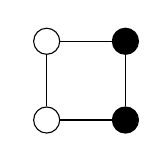
\begin{tikzpicture}
        \node[shape=circle,draw=black,fill=black] (A) at (1,0){};
        \node[shape=circle,draw=black,fill=black] (B) at (1,1){};
        \node[shape=circle,draw=black] (C) at (0,1){}; 
        \node[shape=circle,draw=black] (D) at (0,0){};
        \path [-](A) edge node[left]{} (B);
        \path [-](B) edge node[left]{} (C);
        \path [-](C) edge node[left]{} (D);
        \path [-](D) edge node[left]{} (A);
    \end{tikzpicture}
    \qquad
    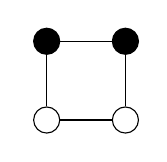
\begin{tikzpicture}
        \node[shape=circle,draw=black] (A) at (1,0) {};
        \node[shape=circle,draw=black,fill=black] (B) at (1,1) {};
        \node[shape=circle,draw=black,fill=black] (C) at (0,1) {};
        \node[shape=circle,draw=black] (D) at (0,0) {};
        \path [-](A) edge node[left]{} (B);
        \path [-](B) edge node[left]{} (C);
        \path [-](C) edge node[left]{} (D);
        \path [-](D) edge node[left]{} (A);
    \end{tikzpicture}
    \qquad
    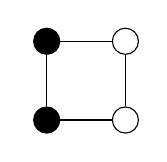
\begin{tikzpicture}
        \node[shape=circle,draw=black] (A) at (1,0) {};
        \node[shape=circle,draw=black] (B) at (1,1) {};
        \node[shape=circle,draw=black,fill=black] (C) at (0,1) {};
        \node[shape=circle,draw=black,fill=black] (D) at (0,0) {};
        \path [-](A) edge node[left]{} (B);
        \path [-](B) edge node[left]{} (C);
        \path [-](C) edge node[left]{} (D);
        \path [-](D) edge node[left]{} (A);
    \end{tikzpicture}
    \qquad
    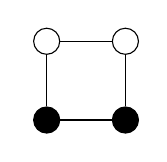
\begin{tikzpicture}
        \node[shape=circle,draw=black,fill=black] (A) at (1,0) {};
        \node[shape=circle,draw=black] (B) at (1,1) {};
        \node[shape=circle,draw=black] (C) at (0,1) {};
        \node[shape=circle,draw=black,fill=black] (D) at (0,0) {};
        \path [-](A) edge node[left]{} (B);
        \path [-](B) edge node[left]{} (C);
        \path [-](C) edge node[left]{} (D);
        \path [-](D) edge node[left]{} (A);
    \end{tikzpicture}
\end{equation}
will be considered equivalent. Let $G=\langle g\rangle$ the cyclic 
group of order four. Let $X$ be 
the set of colorings of the square. Then 
$|X|=16$. 

Let $g$ act on $X$ by anti-clockwise rotations  
of 90\textdegree. All the colorings of~\eqref{eq:orbita} belong to the same orbit. 
Another orbit of $X$ is
\[
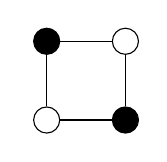
\begin{tikzpicture}
    \node[shape=circle,draw=black,fill=black] (A) at (1,0) {};
    \node[shape=circle,draw=black] (B) at (1,1) {};
    \node[shape=circle,draw=black,fill=black] (C) at (0,1) {};
    \node[shape=circle,draw=black] (D) at (0,0) {};
    \path [-](A) edge node[left]{} (B);
    \path [-](B) edge node[left]{} (C);
    \path [-](C) edge node[left]{} (D);
    \path [-](D) edge node[left]{} (A);
\end{tikzpicture}
\qquad
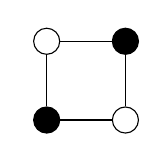
\begin{tikzpicture}
    \node[shape=circle,draw=black] (A) at (1,0) {};
    \node[shape=circle,draw=black,fill=black] (B) at (1,1) {};
    \node[shape=circle,draw=black] (C) at (0,1) {};
    \node[shape=circle,draw=black,fill=black] (D) at (0,0) {};
    \path [-](A) edge node[left]{} (B);
    \path [-](B) edge node[left]{} (C);
    \path [-](C) edge node[left]{} (D);
    \path [-](D) edge node[left]{} (A);
\end{tikzpicture}
\]

Cauchy--Frobenius--Burnside theorem states that
there are  
\[
\frac{1}{|G|}\sum_{x\in G}|\Fix(x)|
\]
orbits. 

For each $x\in G=\{1,g,g^2,g^3\}$ we compute $\Fix(x)$. The identity fixes 
the 16 elements of $X$, both 
$g$ and  $g^3$ fix only two elements of $X$ and 
$g^2$ fixes four elements of $X$. For example, 
the elements of $X$ fixed by $g^2$ are 
\[
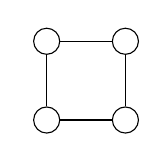
\begin{tikzpicture}
    \node[shape=circle,draw=black] (A) at (1,0){};
    \node[shape=circle,draw=black] (B) at (1,1){};
    \node[shape=circle,draw=black] (C) at (0,1){}; 
    \node[shape=circle,draw=black] (D) at (0,0){};
    \path [-](A) edge node[left]{} (B);
    \path [-](B) edge node[left]{} (C);
    \path [-](C) edge node[left]{} (D);
    \path [-](D) edge node[left]{} (A);
\end{tikzpicture}
\qquad
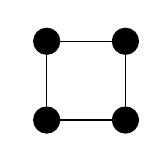
\begin{tikzpicture}
    \node[shape=circle,draw=black,fill=black] (A) at (1,0) {};
    \node[shape=circle,draw=black,fill=black] (B) at (1,1) {};
    \node[shape=circle,draw=black,fill=black] (C) at (0,1) {};
    \node[shape=circle,draw=black,fill=black] (D) at (0,0) {};
    \path [-](A) edge node[left]{} (B);
    \path [-](B) edge node[left]{} (C);
    \path [-](C) edge node[left]{} (D);
    \path [-](D) edge node[left]{} (A);
\end{tikzpicture}
\qquad
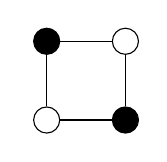
\begin{tikzpicture}
    \node[shape=circle,draw=black,fill=black] (A) at (1,0) {};
    \node[shape=circle,draw=black] (B) at (1,1) {};
    \node[shape=circle,draw=black,fill=black] (C) at (0,1) {};
    \node[shape=circle,draw=black] (D) at (0,0) {};
    \path [-](A) edge node[left]{} (B);
    \path [-](B) edge node[left]{} (C);
    \path [-](C) edge node[left]{} (D);
    \path [-](D) edge node[left]{} (A);
\end{tikzpicture}
\qquad
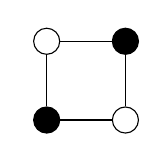
\begin{tikzpicture}
    \node[shape=circle,draw=black] (A) at (1,0) {};
    \node[shape=circle,draw=black,fill=black] (B) at (1,1) {};
    \node[shape=circle,draw=black] (C) at (0,1) {};
    \node[shape=circle,draw=black,fill=black] (D) at (0,0) {};
    \path [-](A) edge node[left]{} (B);
    \path [-](B) edge node[left]{} (C);
    \path [-](C) edge node[left]{} (D);
    \path [-](D) edge node[left]{} (A);
\end{tikzpicture}
\]
Thus $X$ is the union of  
\[
\frac{1}{|G|}\sum_{x\in G}|\Fix(x)|=\frac{1}{4}(16+2+4+2)=6
\]
orbits. 
\end{example}

\begin{exercise}
    In how many ways (up to symmetry) can you
    arrange eight non-attacking rooks on a chessboard? Symmetries 
    are given by the dihedral group $\D_4$ of eight elements.
\end{exercise}

There are 5282 ways (up to symmetry) to arrange 
eight non-attacking rooks on a chessboard. 

\subsection{Commuting probability}

\index{Group commutativity}
For a finite group $G$, let $\cp(G)$ be the probability 
that two random elements of $G$ commute. This number
is also known as the \emph{commutativity} of $G$. 
As an application of Cauchy--Frobenius--Burnside theorem, we
prove that 
$\cp(G)=k/|G|$, where $k$ is the number of conjugacy classes
of $G$. Let 
\[
C=\{(x,y)\in G\times G:xy=yx\}.
\]
We claim that  
    \[
    \cp(G)=\frac{|C|}{|G|^2}=\frac{k}{|G|}.
    \]

Let $G$ act on $G$ by conjugation. 
    By Cauchy--Frobenius--Burnside theorem, 
    \[
    k=\frac{1}{|G|}\sum_{g\in G}|\Fix(g)|=\frac{1}{|G|}\sum_{g\in G}|C_G(g)|=\frac{|C|}{|G|},
    \]
    as $\Fix(g)=\{x\in G:gxg^{-1}=x\}=C_G(g)$ and $\sum_{g\in G}|C_G(g)|=|C|$. 
Alternatively, using Theorem \ref{thm:Frobenius_tau(g)} with $g = 1$,
\[
    \cp(G) = \frac{\tau(1)}{|G|^2} = \frac{1}{|G|}\sum_{\chi \in \Irr(G)} 1 = \frac{k}{|G|},
\]
as $k=|\Irr(G)|$. 
\begin{theorem}
\index{Theorem!5/8}
\label{thm:5/8}
    If $G$ is a non-abelian finite group, then $\cp(G)\leq5/8$.
\end{theorem}

\begin{proof}
%
%    We now claim that $k/|G|\leq 5/8$ if $G$ is non-abelian.
    Let $y_1,\dots,y_m$ the representatives of conjugacy classes of $G$ 
    of size $\geq2$. By the class equation, 
    \[
    |G|=|Z(G)|+\sum_{i=1}^m(G:C_G(y_i))\geq |Z(G)|+2m.
    \]
    Thus $m\leq(1/2)(|G|-|Z(G)|)$ and hence 
    \[
    k=|Z(G)|+m\leq |Z(G)|+\frac12(|G|-|Z(G)|)=\frac12(|Z(G)|+|G|).
    \]
    Since $G$ is non-abelian, $G/Z(G)$ is not cyclic. In particular, 
    $(G:Z(G))\geq4$. Therefore
    \[
    k\leq\frac12(|Z(G)|+|G|)\leq\frac12\left(\frac14+1\right)|G|,
    \]
    that is $k/|G|\leq 5/8$. 
\end{proof}

\begin{exercise}\
\begin{enumerate}
    \item Prove that $\cp(Q_8)=5/8$. 
    \item Prove that $\cp(\Alt_5)=1/12$. 
\end{enumerate}
\end{exercise}

\begin{exercise}
\label{xca:least_p}
    Let $G$ be a finite non-abelian group and $p$ be the smallest prime number
    dividing $|G|$. Prove that $\cp(G)\leq (p^2+p-1)/p^3$. Moreover, 
    the equality holds if and only if $(G:Z(G))=p^2$. 
\end{exercise}

\begin{exercise}
    Let $G$ be a finite group and $H$ be a subgroup of $G$.
    \begin{enumerate}
        \item $\cp(G)\leq\cp(H)$.
        \item If $H$ is normal in $G$, then $\cp(G)\leq\cp(G/H)\cp(H)$.
    \end{enumerate}
\end{exercise}

Degrees of irreducible characters give a lower bound:

\begin{proposition}
If $G$ is a finite group, then
\[
\cp(G)\geq\left(\frac{\sum_{\chi\in\Irr(G)}\chi(1)}{|G|}\right)^2.
\]
\end{proposition}

\begin{proof}
    Let $k$ be the number of conjugacy classes of $G$.
    By Cauchy--Schwarz inequality, 
    \begin{align*}
        \left(\sum_{\chi\in\Irr(G)}\chi(1)\right)^2
        &\leq\left(\sum_{\chi\in\Irr(G)}\chi(1)^2\right)\left(\sum_{\chi\in\Irr(G)}1\right)
        =\left(\sum_{\chi\in\Irr(G)}\chi(1)^2\right)k=|G|k.
    \end{align*}
    From this, the claim follows.
\end{proof}

Using basic facts about irreducible characters, 
we obtain a generalization of Theorem \ref{thm:5/8}. 

\begin{theorem}
\label{thm:[GG]}
    Let $G$ be a finite group. Then
    \[
    |[G,G]|\leq 3/(4\cp(G)-1).
    \]
\end{theorem}

\begin{proof}
    For $n\in\Z_{>0}$, let $\rho_n$ be the number
    of irreducible characters of degree $n$. Then 
    the number of conjugacy classes of $G$ is $k=\sum_{i\geq1}\rho_i$
    and $|G|=\sum_{i\geq1}i^2\rho_i$. 
    It follows that 
    \begin{align*}
    |G|-\rho_1 &=\sum_{i\geq 2}i^2\rho_i\geq 4\sum_{i\geq2}\rho_i
    =4(k-\rho_1)=4(|G|\cp(G)-\rho_1).
    \end{align*}
    Since $\rho_1=(G:[G,G])$, 
    \[
    \cp(G)\leq \frac14+\frac34\frac{\rho_1}{|G|}=\frac14+\frac3{4|[G,G]|}.
    \]
    From this, the claim follows. 
\end{proof}

\begin{exercise}
    \label{xca:5/8}
    Use Theorem \ref{thm:[GG]} to prove Theorem \ref{thm:5/8}.
\end{exercise}

Theorem \ref{thm:[GG]} 
can also be used to
prove similar statements. 

\begin{exercise}
    \label{xca:cp_NS}
    Let $G$ be a finite group. Prove the following statements:
    \begin{enumerate}
        \item If $\cp(G)>1/2$, then $G$ is nilpotent.
        \item If $\cp(G)>21/80$, then $G$ is solvable. 
    \end{enumerate}
\end{exercise}

In the following exercise, we will discuss the notion 
of isoclinic groups. We first need
a preliminary result:

\begin{exercise}
\index{Commutator map}
\label{xca:commutator_map}
    Let $G$ be a group. Prove that the commutator map
    \[
    c_G\colon G/Z(G)\times G/Z(G)\to [G,G],
    \quad
    c_G(xZ(G),yZ(G))=[x,y],
    \]
    is well-defined. 
\end{exercise}

The idea is that two groups are said to be isoclinic 
if their commutator functions are somewhat equal. 

\begin{exercise}
\index{Isoclinism}
\label{xca:isoclinism}
    Let $G$ and $H$ be groups. 
    A pair $(\sigma,\tau)$ of maps is an \emph{isoclinism}
    between $G$ and $H$ if 
    $\sigma\colon G/Z(G)\to H/Z(H)$ and  
    $\tau\colon [G,G]\to [H,H]$ are group isomorphisms and 
    the diagram
    \begin{equation}
    \label{eq:isoclinism}
    \begin{tikzcd}
	{G/Z(G)\times G/Z(G)} & {H/Z(H)\times H/Z(H)} \\
	{[G,G]} & {[H,H]}
	\arrow["{\sigma\times\sigma }", from=1-1, to=1-2]
	\arrow["{c_H}", from=1-2, to=2-2]
	\arrow["{c_G}"', from=1-1, to=2-1]
	\arrow["\tau"', from=2-1, to=2-2]
    \end{tikzcd}
    \end{equation} 
    commutes. We write $G\sim H$ when there exists 
    an isoclinism between $G$ and $H$. 
    
    Prove the following statements:
    \begin{enumerate}
        \item If $G\simeq H$, then $G\sim H$.
        \item If $G\sim H$, then $\cp(G)=\cp(H)$. 
    \end{enumerate}
\end{exercise}

\begin{exercise}
\label{xca:isoclinism_simple}
    Let $S$ be a non-abelian simple group and
    $G$ be a group such that $G\sim S$. Prove that 
    $G\simeq S\times A$ for some abelian group $A$.
\end{exercise}

\begin{exercise}
\label{xca:isoclinism_factorization}
    Let $H$ be a subgroup of $G$. If $G=HZ(G)$, then $G\sim H$. 
    Conversely, if $G\sim H$ and $H$ is finite, then 
    $G=HZ(G)$. 
\end{exercise}

The following theorem appeared in 1970 as a problem in 
volume 13 of the \textit{Canadian Math. Bulletin}. The solution
appeared in 1973. 
Iv\'an Sadosfchi Costa found the proof we present here. 

\begin{theorem}[Dixon]
    \index{Dixon's theorem}
    The commuting probability of every finite 
    non-abelian simple group is at most $1/12$. 
   %If $G$ is a finite non-abelian simple group, then $\cp(G)\leq1/12$.
\end{theorem}

\begin{proof}
Let $G$ be a finite non-abelian simple group. We claim that 
$\cp(G)\leq1/12$. 
We assume that $\cp(G)>1/12$. Since
$G$ is a non-abelian simple group, 
the identity of $G$ is the only central element of $G$. 

Let us assume first that there is a conjugacy class of $G$ of size $m$, where
$m$ is such that $1<m\leq 12$. Then $G$ is a transitive subgroup of $\Sym_m$.
For these groups, the problem is easy: we show that there are no non-abelian simple groups
that act transitively on sets of size $m\in\{2,\dots,12\}$ with commuting
probability $>1/12$. To do this, we list these transitive groups and their commuting
probabilities and verify that all commuting probabilities are $\leq
1/12$:
\begin{lstlisting}
gap> l := AllTransitiveGroups(NrMovedPoints, [2..12], \\
> IsAbelian, false, IsSimple, true);;
[ A5, L(6) = PSL(2,5) = A_5(6), A6, 
  L(7) = L(3,2), A7, L(8)=PSL(2,7), A8, 
  L(9)=PSL(2,8), A9, A_5(10), L(10)=PSL(2,9), 
  A10, L(11)=PSL(2,11)(11), M(11), A11, A_5(12), 
  L(2,11), M_11(12), M(12), A12 ]
gap> List(l, CommutingProbability);           
[ 1/12, 1/12, 7/360, 1/28, 1/280, 1/28, 1/1440, 
  1/56, 1/10080, 1/12, 7/360, 1/75600, 2/165, 
  1/792, 31/19958400, 1/12, 2/165, 1/792, 1/6336, 
  43/239500800 ]
gap> ForAny(l, x->CommutingProbability(x)>1/12);
false
\end{lstlisting}

Now assume that all non-trivial conjugacy classes of $G$ have at least 13 elements. Let $k$ be the number of conjugacy classes of $G$. 
Then the class equation implies that
\begin{align*}
	|G|&\geq 1+(k-1)13=13k-12.
\end{align*}
Since $\cp(G)=k/|G|>1/12$, $k>|G|/12$. Thus 
\[
|G|>\frac{13}{12}|G|-12
\]
and therefore $|G|<144$. Thus one needs to check what happens with groups
of order $<144$. 
But we know that the only non-abelian simple group of size
$<144$ is the alternating simple group $\Alt_5$.
\begin{lstlisting}
gap> AllGroups(Size, [2..143], \\
> IsAbelian, false, \\
> IsSimple, true);
[ Alt( [ 1 .. 5 ] ) ]
\end{lstlisting}    
This completes the proof. 
\end{proof}

The alternating group $\Alt_5$ is important in this setting:

\begin{theorem}[Guralnick--Robinson]
    \index{Guralnick--Robinson theorem}
    If $G$ is a finite non-solvable group such that $\cp(G)>3/40$, then
    $G\simeq\Alt_5\times T$ for some abelian group 
    $T$ and $\cp(G)=1/12$. 
\end{theorem}

The proof appears in~\cite{MR2228209}.

Results on probability of commuting elements generalize in other directions. 
In~\cite{MR230809,MR276325,MR313378,MR369512}, 
Thompson proved the following result:

\begin{theorem}[Thompson]
\index{Thompson's theorem}
    If $G$ is a finite group such that 
    every pair of elements of $G$ generate
    a solvable group, then $G$ is solvable. 
\end{theorem}

The proof uses the classification of finite simple groups (CFSG). A simpler
proof independent of the CFSG appears in~\cite{MR1346207}.

There is a probabilistic version of Thompson's theorem:

\begin{theorem}[Guralnick--Wilson]
    \index{Guralnick--Wilson theorem}
    Let $G$ be a finite group.
    \begin{enumerate}
        \item If the probability that two random elements of $G$ 
        generate a solvable group is $>11/30$, then $G$ is solvable. 
        \item If the probability that two random elements of $G$ 
        generate a nilpotent group is $>1/2$, then $G$ is nilpotent.
        \item If the probability that two random elements of $G$ 
        generate a group of odd order is $>11/30$, then $G$ has odd order.
    \end{enumerate}
\end{theorem}

The proof uses the CFSG and appears in~\cite{MR1770615}.

\subsection{Jordan's theorem and applications}

We now follow~\cite{MR1997347} to present other applications. 

\begin{theorem}[Jordan]
\index{Jordan's theorem}
    Let $G$ be a non-trivial finite group. If $G$ acts transitively 
    on a finite set $X$ and $|X|>1$, then there exists 
    $g\in G$ with no fixed points.
\end{theorem}

\begin{proof}
    Cauchy--Frobenius--Burnside theorem implies that
    \[
    1=\frac{1}{|G|}\sum_{g\in G}|\Fix(g)|=\frac{1}{|G|}\left(|X|+\sum_{g\ne 1}|\Fix(g)|\right).
    \]
    If every $g\in G\setminus\{1\}$ contains at least one fixed-point, then
    \[
    1=\frac{1}{|G|}\left(|X|+\sum_{g\ne 1}|\Fix(g)|\right)\geq \frac{1}{|G|}(|X|+|G|-1)=1+\frac{|X|-1}{|G|}
    \]
    and thus $|X|\leq1$, a contradiction. 
\end{proof}

\begin{corollary}
    Let $G$ be a finite group and $H$ be a proper subgroup of $G$. 
    Then $G\ne\cup_{g\in G}gHg^{-1}$.
\end{corollary}

\begin{proof}
    The group $G$ acts transitively by left multiplication on $X=G/H$. The stabilizer
    of $xH$ is 
    \[
    G_{xH}=\{g\in G:gxH=xH\}=xHx^{-1}.
    \]
    Since $H\ne G$, it follows that $|X|=|G/H|>1$. Jordan's theorem now implies
    that there exists $g\in G$ with no fixed-points, that is 
    there is an element $g\in G$ such that $g\not\in\cup_{x\in G}xHx^{-1}$. 
\end{proof}

Let $G$ be a finite group. We say that the conjugacy classes $C$ and $D$ 
\emph{commute} if there exist 
$c\in C$ and $d\in D$ such that $[c,d]=1$. 
Note that $C$ and $D$ commute if and only if for all $c\in C$ there exists $d\in D$ 
such that $[c,d]=1$. 

\begin{corollary}[Wildon]
\index{Wildon's theorem}
    Let $G$ be a finite group and $C$ be a conjugacy class of $G$. 
    Then $|C|=1$ if and only if $C$ commutes 
    with every conjugacy class of $G$.
\end{corollary}
    
\begin{proof}
    We prove $\impliedby$. 
    Assume that $C$ commutes with every conjugacy class of $G$. 
    Let $c\in C$ and $H=C_G(c)$. Then $H\cap D\ne\emptyset$ for every conjugacy class
    $D$. We claim that $G=\cup_{g\in G}gHg^{-1}$. In fact, let $x\in G$. Then
    $x\in D$ 
    for some conjugacy class $D$. 
    Let 
    $h\in H\cap D$. There exists $y\in G$ such that $h=yxy^{-1}$, that is
    $x=y^{-1}hy\in \cup_{g\in G}gHg^{-1}$. By Jordan's theorem,  
    $H=G$. Thus $c$ is central and hence $C=\{c\}$. 
    
    We now prove $\implies$. If $C=\{c\}$, then $c\in Z(G)$ and $C$ commute with every 
    conjugacy class of~$G$. 
\end{proof}

With the CFSG one proves a result similar to that of Jordan. 

\begin{theorem}[Fein--Kantor--Schacher]
    \index{Fein--Kantor--Schacher theorem}
    Let $G$ be a non-trivial finite group. If $G$ acts transitively
    on a finite set $X$ and $|X|>1$, then
    there exist a prime number $p$ and an element $g\in G$ with no fixed-points
    with order a power of $p$.
\end{theorem}

The proof appears in~\cite{MR636194}. 

\subsection{Derangements: Cameron--Cohen theorem}

\index{Derangements}
Let $G$ be a finite group that acts faithfully and transitively 
on a finite set $X$, say 
$G\leq\Sym_n$, where $X=\{1,2,\dots,n\}$. Let 
$G_0$ be the set of elements $g\in G$ with no fixed-points, 
that is $g(x)\ne x$ for all $x\in X$. 
Such permutations are known as \emph{derangements}. 
Let $c_0=|G_0|/|G|$. 

\begin{theorem}[Cameron--Cohen]
    \index{Cameron--Cohen theorem}
    If $G$ is a subgroup of $\Sym_n$ that acts transitively on 
    $\{1,\dots,n\}$, then $c_0\geq\frac{1}{n}$.
\end{theorem}

\begin{proof}
    Let $X=\{1,\dots,n\}$. By definition, the rank of $G$ is the number
    of orbitals of $G$ on $X$. It follows that the rank is $\geq2$, as
    $X\times X$ decomposes as 
    \[
    X\times X=\Delta\cup\left((X\times X)\setminus\Delta\right)
    \]
    Let $\chi(g)=|\Fix(g)|$ and $G_0=\{g\in G:\chi(g)=0\}$. If $g\not\in G_0$, then $1\leq\chi(g)\leq n$. Since  
    $(\chi(g)-1)(\chi(g)-n)\leq 0$,
    \[
    \frac{1}{|G|}\sum_{g\in G\setminus G_0}(\chi(g)-1)(\chi(g)-n)\leq 0.
    \]
    On the one hand, 
    \begin{align*}
    \frac{1}{|G|}\sum_{g\in G}(\chi(g)&-1)(\chi(g)-n)\\
    &=\frac{1}{|G|}\left\{\sum_{g\in G_0}+\sum_{g\in G\setminus G_0}\right\}(\chi(g)-1)(\chi(g)-n)\\
    &\leq n\frac{|G_0|}{|G|}=nc_0.
    \end{align*}
    On the other hand, since the rank of $G$ is $\geq2$, 
    \begin{equation}
        \label{eq:CameronCohen}
        2-\frac{n+1}{|G|}\sum_{g\in G}\chi(g)+n\leq 
        \frac{1}{|G|}\sum_{g\in G}(\chi(g)-1)(\chi(g)-n)\leq nc_0.
    \end{equation}
    Since $G$ is transitive on $X$, Cauchy--Frobenius--Burnside theorem implies that
    $\sum_{g\in G}\chi(g)=|G|$. Thus $2-(n+1)+n\leq nc_0$ and hence
    $1/n\leq c_0$. 
\end{proof}

Cameron--Cohen theorem contains another claim: If
$n$ is not the power of a prime number, then 
$c_0>1/n$. The proof uses Frobenius' theorem. 

With the CFSG the bound in 
Cameron--Cohen theorem can be improved:

\begin{theorem}[Guralnick--Wan]
    \index{Guralnick--Wan theorem}
    Let $G$ be a finite transitive group of degree $n\geq2$. If $n$ 
    is not a power of a prime number and 
    $G\ne\Sym_n$ for $n\in\{2,4,5\}$, then $c_0\geq 2/n$.
\end{theorem}

The proof appears in~\cite{MR1484879} and uses
the classification of finite 2-transitive groups, 
which depends on the CFSG. 




\section{Lecture: Week 7}

\subsection{The Brauer--Fowler theorem}

\index{Symmetric}
\index{Antisymmetric}
Let $\rho\colon G\to\GL(V)$ 
be a representation with character $\chi$. The $\C[G]$-module $V\otimes V$ 
has character $\chi^2$. Let 
$\{v_1,\dots,v_n\}$ be a basis of $V$ and 
\[
T\colon V\otimes V\to V\otimes V,\quad
v_i\otimes v_j\mapsto v_j\otimes v_i.
\]
It is an exercise to check that 
\[
T(v\otimes w)=w\otimes v
\]
for all 
$v,w\in V$. (Thus 
$T$ does not depend on the basis $\{v_1,\dots,v_n\}$.) Note that
$T$ is a homomorphism of $\C[G]$-modules, as
\[
T(g\cdot (v\otimes w))=T((g\cdot v)\otimes (g\cdot w))=(g\cdot w)\otimes (g\cdot v)=g\cdot T(v\otimes w)
\]
for all $g\in G$ y $v,w\in V$. 
In particular, the \emph{symmetric part} 
\begin{gather*}
S(V\otimes V)=\{x\in V\otimes V:T(x)=x\}
\shortintertext{and the \emph{antisymmetric} part}
A(V\otimes V)=\{x\in V\otimes V:T(x)=-x\}
\end{gather*}
of $V\otimes V$ are both  
$\C[G]$-submodules of $V\otimes V$. 
The terminology is motivated by the following fact:
\[
V\otimes V=S(V\otimes V)\oplus A(V\otimes V).
\]
In fact, 
$S(V\otimes V)\cap A(V\otimes V)=\{0\}$, as   
$x\in S(V\otimes V)\cap A(V\otimes V)$ implies
$x=T(x)$ and $x=-T(x)$. Hence $x=0$. Moreover, 
$V\otimes V=S(V\otimes V)+ A(V\otimes V)$, as every $x\in V\otimes V$ can be written 
as 
\[
x=\frac12(x+T(x))+\frac12(x-T(x))
\]
with $\frac12(x+T(x))\in S(V\otimes V)$ and $\frac12(x-T(x))\in A(V\otimes V)$. 

We claim that 
\[
\{v_i\otimes v_j+v_j\otimes v_i:1\leq i\leq j\leq n\}
\]
is
a basis of $S(V\otimes V)$, 
and that  
\[
\{v_i\otimes v_j-v_j\otimes v_i:1\leq i<j\leq n\}
\]
is a basis of $A(V\otimes V)$. Since both sets are linearly independent, 
\[
\dim S(V\otimes V)\geq n(n+1)/2\text{ and }
\dim A(V\otimes V)\geq n(n-1)/2.
\]
Moreover, 
\[
n^2=\dim (V\otimes V)=\dim S(V\otimes V)+\dim A(V\otimes V),
\]
so it follows that
$\dim S(V\otimes V)=n(n+1)/2$ and $\dim A(V\otimes V)=n(n-1)/2$. 

\begin{proposition}
\label{pro:SandA}
    Let $G$ be a finite group and
    $V$ be a finite-dimensional 
    $\C[G]$-module with character $\chi$. If $S(V\otimes V)$ 
    has character $\chi_S$ and $A(V\otimes V)$ has character
    $\chi_A$, then 
    \begin{align*}
        &\chi_S(g)=\frac12(\chi^2(g)+\chi(g^2)) && \text{and} &&
        \chi_A(g)=\frac12(\chi^2(g)-\chi(g^2)).
    \end{align*}
\end{proposition}

\begin{proof}
    Let $g\in G$ and $\rho\colon G\to\GL(V)$ be the representation
    associated with $V$, that is $\rho(g)(v)=\rho_g(v)=g\cdot v$. 
    Since $\rho_g$ is diagonalizable, let $\{e_1,\dots,e_n\}$ 
    be a basis of eigenvectors of $\rho_g$, say
    $g\cdot e_i=\lambda_ie_i$ with $\lambda_i\in\C$ for all $i\in\{1,\dots,n\}$. In particular, $\chi(g)=\sum_{i=1}^n\lambda_i$. 
    
    Since $\{e_i\otimes e_j-e_j\otimes e_i:1\leq i<j\leq n\}$ is a basis of
    $A(V\otimes V)$ and 
    \[
    g\cdot (e_i\otimes e_j-e_j\otimes e_i)=\lambda_i\lambda_j(e_i\otimes e_j-e_j\otimes e_i),
    \]
    it follows that
    \[
    \chi_A(g)=\sum_{1\leq i<j\leq n}\lambda_i\lambda_j.
    \]
    On the other hand,
    $g^2\cdot e_i=\lambda_i^2e_i$ for all $i$,
    $\chi(g^2)=\sum_{i=1}^n\lambda_i^2$. Thus 
    \[
    \chi^2(g)=\chi(g)^2=\sum_{i=1}^n\sum_{j=1}^n\lambda_i\lambda_j=2\sum_{1\leq i<j\leq n}\lambda_i\lambda_j+\sum_{i=1}^n\lambda_i^2=2\chi_A(g)+\chi(g^2).
    \]
    Since $V\otimes V=S(V\otimes V)\oplus A(V\otimes V)$, it follows that  
    $\chi^2(g)=\chi_S(g)+\chi_A(g)$, that is 
    $\chi_S(g)=\frac12(\chi^2(g)+\chi(g^2))$.
\end{proof}

\index{Involution}
An \emph{involution} of a group is an element $x\ne 1$ such that $x^2=1$. 
It is possible to use the character table to count the number
of involutions.

\begin{proposition}
    If $G$ is a finite group with $t$ involutions, then
    \[
        1+t=\sum_{\chi\in\Irr(G)}\langle\chi_S-\chi_A,\chi_1\rangle\chi(1),
    \]
    where $\chi_1$ is 
    the trivial character of $G$.
\end{proposition}

\begin{proof}
    Assume that $\Irr(G)=\{\chi_1,\dots,\chi_k\}$.  
    For $x\in G$ let 
    \[
    \theta(x)=|\{y\in G:y^2=x\}|.
    \]
    Since $\theta$ is a class function, 
    $\theta$ is a linear combination of the $\chi_j$'s, say 
    \[
    \theta=\sum_{\chi\in\Irr(G)}\langle\theta,\chi\rangle\chi.
    \]
    For every $\chi\in\Irr(G)$ we compute: 
    \begin{align*}
        \langle\chi_S-\chi_A,\chi_1\rangle 
        &=\frac{1}{|G|}\sum_{g\in G}\chi(g^2)\\
        &=\frac{1}{|G|}\sum_{x\in G}\sum_{\substack{g\in G\\g^2=x}}\chi(g^2)
        =\frac{1}{|G|}\sum_{x\in G}\theta(x)\chi(x)=\langle\theta,\chi\rangle.
    \end{align*}
    Thus $\theta=\sum_{\chi\in\Irr(G)}\langle\chi_S-\chi_A,\chi_1\rangle\chi$. Now
    the claim follows after evaluating this expression in 
    $x=1$. 
\end{proof}

\index{Cauchy--Schwarz inequality}
Before proving the Brauer--Fowler theorem, we
need a lemma. We will use the Cauchy--Schwarz inequality: 
\[
x_1,\dots,x_n\in\R\implies
\sum x_i^2\geq\frac{1}{n}(\sum x_i)^2.
\]

\begin{lemma}
    Let $G$ be a finite group with $k$ conjugacy classes. 
    If $t$ is the number of involutions of $G$, then
    $t^2\leq (k-1)(|G|-1)$. 
\end{lemma}

\begin{proof}
    Assume that $\Irr(G)=\{\chi_1,\dots,\chi_k\}$, where $\chi_1$ is the
    trivial character of $G$. 
    If $\chi\in\Irr(G)$, then 
    \[
        \langle\chi^2,\chi_1\rangle=\frac{1}{|G|}\sum_{g\in G}\chi(g)\chi(g)=\langle\chi,\overline{\chi}\rangle=\begin{cases}
        1 & \text{if $\chi=\overline{\chi}$},\\
        0 & \text{otherwise}.
        \end{cases}
    \]
    Since $\chi^2=\chi_S+\chi_A$, if $\langle\chi^2,\chi_1\rangle=1$, then
    the trivial character either is part of $\chi_S$ or $\chi_A$, but not both. 
    Thus
    \[
    \langle\chi_S-\chi_A,\chi_1\rangle\in\{-1,1,0\}.
    \]
    
    We claim that 
    $t\leq\sum_{i=2}^k\chi_i(1)$. In fact, since 
    $|\langle\chi_S-\chi_A,\chi_1\rangle|\leq 1$, 
    \begin{align*}
        1+t=\theta(1)
        &=\left|\sum_{\chi\in\Irr(G)}\langle\chi_S-\chi_A,\chi_1\rangle\chi(1)\right|\\
        &\leq\sum_{\chi\in\Irr(G)}|\langle\chi_S-\chi_A,\chi_1\rangle|\chi(1)
        \leq\sum_{\chi\in\Irr(G)}\chi(1).
    \end{align*}
    It follows that $t\leq\sum_{i=2}^k\chi_i(1)$. 
    By the Cauchy--Schwarz inequality, 
    \[
        t^2\leq\left(\sum_{i=2}^k\chi_i(1)\right)^2
        \leq(k-1)\sum_{i=2}^k\chi(1)^2=(k-1)(|G|-1).\qedhere
    \]
\end{proof}

Now we prove the Brauer--Fowler theorem. 

\begin{theorem}[Brauer--Fowler]
    \index{Brauer--Fowler theorem}
    Let $G$ be a finite simple group and $x$ be an involution of $G$. If $|C_G(x)|=n$, then $|G|\leq (n^2)!$	
\end{theorem}

\begin{proof}
    If $G$ is abelian, the claim is trivial. Let $G$ be a finite non-abelian simple group.
    We first assume the existence of a proper subgroup $H$ of $G$ 
    such that 
    \[
    (G:H)\leq n^2.
    \]
    Let $G$ act on $G/H$ 
    by left multiplication, and let 
    $\rho\colon G\to\Sym_{n^2}$ be the corresponding
    group homomorphism. Since $G$ is simple, either 
    $\ker\rho=\{1\}$ or $\ker\rho=G$. If $\ker\rho=G$, then
    $\rho(g)(yH)=yH$ for all $g\in G$ and $y\in G$. 
    Hence $H=G$, a contradiction. Therefore $\rho$ is injective
    and hence $G$ is isomorphic to a subgroup of $\Sym_{n^2}$. 
    In particular, $|G|$ divides $(n^2)!$. 

    Let $m=(|G|-1)/t$, where $t$ is the number of involutions of $G$. 
    Since $|C_G(x)|=n$, the group $G$ has at least $|G|/n$ involutions (because
    the conjugacy class of $x$ has size $|G|/n$ and all its elements are involutions), 
    that is $t\geq |G|/n$. Hence 
    \[
    m=(|G|-1)/t<n.
    \]
    It is enough to show that
    $G$ contains a subgroup of index $\leq m^2$. 

    Let $C_1,\dots,C_k$ be the conjugacy classes of $G$, where $C_1=\{1\}$. 
    Since $G$ is simple and non-abelian, $|C_i|>1$ 
    for all $i\in\{2,\dots,k\}$. By the previous lemma, 
    \[
    t^2\leq(k-1)(|G|-1)\implies |G|-1=\frac{mt^2}{t}\leq\frac{(k-1)(|G|-1)^2}{t^2}=(k-1)m^2.
    \]
    If $|C_i|>m^2$ for all $i\in\{2,\dots,k\}$, then
    \[
    |G|-1=\sum_{i=2}^k|C_i|>(k-1)m^2,
    \]
    a contradiction. Thus there exists a non-trivial conjugacy class
    $C$ of $G$ such that $|C|\leq m^2$. If $g\in C$, then
    $C_G(g)$ is a proper subgroup of $G$ of index $|C|\leq m^2$.
\end{proof}

The bound of the Brauer--Fowler theorem is not essential.
What matters is the following consequence:

\begin{corollary}
    Let $n\geq 1$ be an integer. There are at most finitely many 
    finite simple groups with an involution with a centralizer of order $n$.
\end{corollary}

As an exercise, a simple application: 

\begin{exercise}
    If $G$ is a finite simple group and $x$ is an involution with
    centralizer of order two, then  
    $G\simeq\Z/2$. 
\end{exercise}

\subsection{The character table of $\Sym_5$}
\index{Character table!of $\Sym_5$}
Let $G=\Sym_5$. The conjugacy classes 
of $G$ are given in the following table:

\bigskip 
\begin{center}
    \begin{tabular}{c|ccccccc}
        Representative & $\id$ & $(12)$ & $(123)$ & $(12)(34)$ & $(1234)$ & $(123)(45)$  & $(12345)$ \\
        \hline 
        Size & $1$ & $10$ & $20$ & $15$ & $30$ & $20$ & $24$ \\
    \end{tabular}
\end{center}
\bigskip 

Thus there are seven irreducible characters. The trivial character $\chi_1$ and the sign $\chi_2$ are degree-one (hence irreducible) 
characters. 

\bigskip 
\begin{center}
    \begin{tabular}{|c|ccccccc|}
        \hline 
        & $\id$ & $(12)$ & $(123)$ & $(12)(34)$ & $(1234)$ & $(123)(45)$  & $(12345)$ \\
        \hline 
        $\chi_1$ & $1$ & $1$ & $1$ & $1$ & $1$ & $1$ & $1$ \\
        $\sgn$ & $1$ & $-1$ & $1$ & $1$ & $-1$ & $-1$ & $1$ \\
        \hline 
    \end{tabular}
\end{center}
\bigskip 

Since 
$[G,G]=\Alt_5$ and $|G/[G,G]|=2$, it follows
from Exercise~\ref{xca:degree-one} that $\chi_1$ and $\sgn$ 
are the only degree-one characters. 

Since $G$ acts 2-transitively on $\{1,\dots,5\}$, Proposition~\ref{pro:2transitive} implies that 
$\varsigma(g)=|\Fix(g)|-1$ is an irreducible character. 
A direct
calculation yields the values of $\varsigma$: 
\bigskip 
\begin{center}
    \begin{tabular}{|c|ccccccc|}
        \hline 
        & $\id$ & $(12)$ & $(123)$ & $(12)(34)$ & $(1234)$ & $(123)(45)$  & $(12345)$ \\
        \hline 
        $\varsigma$ & $4$ & $2$ & $1$ & $0$ & $0$ & $-1$ & $-1$ \\
        \hline 
    \end{tabular}
\end{center}
\bigskip 

The values of the product 
$\sgn\varsigma$ are easily computed: 
\bigskip 
\begin{center}
    \begin{tabular}{|c|ccccccc|}
        \hline 
        & $\id$ & $(12)$ & $(123)$ & $(12)(34)$ & $(1234)$ & $(123)(45)$  & $(12345)$ \\
        \hline 
        $\sgn\varsigma$ & $4$ & $-2$ & $1$ & $0$ & $0$ & $1$ & $-1$ \\
        \hline 
    \end{tabular}
\end{center}
\bigskip 

Since 
\begin{align*}
\langle\sgn\varsigma,\sgn\varsigma\rangle&=
\frac{1}{120}(4^2+10(-2)^2+20+15\cdot 0+30\cdot 0+20+24)\\
&=\frac{1}{120}(16+40+20+20+24)=1,
\end{align*}
it follows that $\sgn\varsigma\in\Irr(G)$. 

We now consider the characters 
\[
\psi(g)=\frac12(\varsigma^2(g)+\varsigma(g^2))\quad\text{and}\quad  
\eta(g)=\frac12(\varsigma^2(g)-\varsigma(g^2)),
\]
where $\varsigma^2(g)=\varsigma(g)\varsigma(g)=\varsigma(g)^2$ (see Proposition~\ref{pro:SandA}). 
A straightforward 
calculation shows that 
\bigskip 
\begin{center}
    \begin{tabular}{|c|ccccccc|}
        \hline 
        & $\id$ & $(12)$ & $(123)$ & $(12)(34)$ & $(1234)$ & $(123)(45)$  & $(12345)$ \\
        \hline 
        $\psi$ & $10$ & $4$ & $1$ & $2$ & $0$ & $1$ & $0$ \\
        $\eta$ & $6$ & $0$ & $0$ & $-2$ & $0$ & $0$ & $1$ \\
        \hline 
    \end{tabular}
\end{center}
\bigskip 

Since 
\[
\langle\eta,\eta\rangle
=\frac{1}{120}(6^2+15(-2)^2+24)=1,
\]
it follows that $\eta\in\Irr(G)$. On the other hand,
\[
\langle\psi,\psi\rangle
=\frac{1}{120}(10^2+10\cdot16+20+15\cdot 4+20)=3. 
\]
Thus $\psi$ is the sum of three irreducible characters (see Exercise~\ref{xca:n_irreducible}). Since 
\begin{align*}
\langle\psi,\chi_1\rangle&=\frac{1}{120}(10+10\cdot 4+20+15\cdot 2+20)=1,\\
\langle\psi,\varsigma\rangle&=\frac{1}{120}(10\cdot 4+10\cdot 4\cdot 2+20-20)=1,
\end{align*}
it follows that 
$\psi=\chi_1+\varsigma+\chi$ for some $\chi\in\Irr(G)$. Thus
we can compute $\chi$:
\bigskip 
\begin{center}
    \begin{tabular}{|c|ccccccc|}
        \hline 
        & $\id$ & $(12)$ & $(123)$ & $(12)(34)$ & $(1234)$ & $(123)(45)$  & $(12345)$ \\
        \hline 
        $\chi$ & $5$ & $1$ & $-1$ & $1$ & $-1$ & $1$ & $0$ \\
        \hline 
    \end{tabular}
\end{center}
\bigskip 
We are missing one irreducible character. Let $n$ be 
the degree of this character. Since 
$120=1+1+16+16+36+25+n^2$, it follows that 
$n=5$. Since we need a degree-five
irreducible character, we can try with
$\xi=\sgn\chi$:
\bigskip 
\begin{center}
    \begin{tabular}{|c|ccccccc|}
        \hline 
        & $\id$ & $(12)$ & $(123)$ & $(12)(34)$ & $(1234)$ & $(123)(45)$  & $(12345)$ \\
        \hline 
        $\xi$ & $5$ & $-1$ & $-1$ & $1$ & $1$ & $-1$ & $0$ \\
        \hline 
    \end{tabular}
\end{center}
\bigskip 

Since 
\[
\langle\xi,\xi\rangle=\frac{1}{120}(25+10(-1)^2+20(-1)^2+15+30+20(-1)^2)
=1,
\]
it follows that $\xi\in\Irr(G)$. We have found the character table of $G$. 

\bigskip 
\begin{center}
    \begin{tabular}{|c|ccccccc|}
        \hline 
        & $\id$ & $(12)$ & $(123)$ & $(12)(34)$ & $(1234)$ & $(123)(45)$  & $(12345)$ \\
        \hline 
        $\chi_1$ & $1$ & $1$ & $1$ & $1$ & $1$ & $1$ & $1$ \\
        $\sgn$ & $1$ & $-1$ & $1$ & $1$ & $-1$ & $-1$ & $1$ \\
        $\varsigma$ & $4$ & $2$ & $1$ & $0$ & $0$ & $-1$ & $-1$ \\
        $\sgn\varsigma$ & $4$ & $-2$ & $1$ & $0$ & $0$ & $1$ & $-1$ \\
        $\eta$ & $6$ & $0$ & $0$ & $-2$ & $0$ & $0$ & $1$ \\
        $\chi$ & $5$ & $1$ & $-1$ & $1$ & $-1$ & $1$ & $0$ \\
        $\xi$ & $5$ & $-1$ & $-1$ & $1$ & $1$ & $-1$ & $0$ \\
        \hline 
    \end{tabular}
\end{center}
\bigskip 

% g=id,(12),(123),(12)(34),(1234),(123)(45),(12345)
% chi_3^2(g) : 16,4,1,0,0,1,1
% chi_3(g^2) : 4,4,1,4,0,1,-1


\subsection{(optional) An elementary proof of the Brauer--Fowler theorem}

We need to find a subgroup of index $\leq 2n^2$. 
Let $X$ be the conjugacy class of $x$. For $g\in G$ let
\[
J(g)=\{z\in X:zgz^{-1}=g^{-1}\}.
\]
We claim that $|J(g)|\leq|C_G(g)|$. The map $J(g)\to C_G(g)$, $z\mapsto gz$, 
is well-defined,~as 
\[
(gz)g(gz)^{-1}=g(zgz^{-1})g^{-1}=g^{-1}\in C_G(g).
\]
It is injective, as $gz=gz_1$ implies $z=z_1$.

Let $J=\{(g,z)\in G\times X:zgz^{-1}=g^{-1}\}$.  
Since $X\times X\to J$, $(y,z)\mapsto (yz,z)$, 
is well-defined (since $z(yz)z^{-1}=zy=(yz)^{-1}$) and
it is trivially injective, 
\[
|X|^2\leq |J|=\sum_{(g,z)\in J}1\leq\sum_{g\in G}|J(g)|
\leq\sum_{g\in G}|C_G(g)|=k|G|,
\]
where $k$ is the number of conjugacy classes of $G$, 
as $(g,z)\in J$ if and only if $z\in J(g)$. Thus $|G|\leq kn^2$, as
\[
\left(\frac{|G|}{|C_G(x)|}\right)^2=|X|^2=\frac{|G|^2}{n^2}\leq k|G|.
\]

\begin{claim}
    There exists a non-trivial conjugacy class with $\leq 2n^2$ elements.
\end{claim}

Assume that the claim is not true. Let
$C_1,\dots,C_k$ be the conjugacy classes of $G$, where 
$C_1=\{1\}$ and $|C_i|>2n^2$ for all $i\in\{2,\dots,k\}$. Then
\[
|G|=1+\sum_{i=2}^k|C_i|>1+\sum_{i=2}^k2n^2=1+(k-1)2n^2\geq |G|,
\]
a contradiction. 

\begin{claim}
    There exists a subgroup $H$ of $G$ such that
    $(G:H)\leq 2n^2$.
\end{claim}

Let $C$ be a conjugacy class of $G$ such that 
$|C|\leq 2n^2$. Let $g\in C$.  
Then $H=C_G(g)$ is a subgroup of $G$ such that
$(G:H)\leq 2n^2$. 
This finishes the proof of the Brauer--Fowler theorem. 



\subsection{Frobenius's reciprocity}

We now present a very quick version of Frobenius'
reciprocity theorem. We first 
define the restriction of class functions. 

\begin{definition}
    Let $G$ be a finite group and $f\colon G\to\C$ be
    a map. For a subgroup $H$ of $G$, the \emph{restriction}
    of $f$ to $H$ is the map 
    $\Res_H^G=f|_H\colon H\to\C$, $h\mapsto f(h)$. 
\end{definition}

\begin{exercise}
\label{xca:restriction}
    Let $G$ be a finite group. Prove that
    the map 
    \[
    \Res_H^G\colon\cf(G)\to\cf(H),\quad  f\mapsto\Res_H^G(f),
    \]
    is a well-defined linear map. 
\end{exercise}

We now define induction. Let $G$ be a finite group
and $H$ be a subgroup of $G$. If $f\colon H\to\C$ is a map, 
then 
\[
f^0(x)=\begin{cases}
    f(x) & \text{if $x\in H$},\\
    0 & \text{otherwise}.
    \end{cases}
\]
It is an exercise to prove that
the map $f\mapsto f^0$ is linear. 

\begin{definition}
    Let $G$ be a finite group and $H$ be a subgroup of $G$. Let
    $f\colon H\to\C$ be
    a map. The \emph{induction}
    of $f$ to $G$ is the map 
    \begin{align*}
      g\mapsto\Ind_H^Gf(g)=\frac{1}{|H|}\sum_{x\in G}f^0(x^{-1}gx).
    \end{align*}
\end{definition}

\begin{exercise}
\label{xca:induction}
    Let $G$ be a finite group. Prove that
    the map 
    \[
    \Ind_H^G\colon\cf(H)\to\cf(G),\quad  f\mapsto\Ind_H^G(f),
    \]
    is a well-defined linear map. 
\end{exercise}

\begin{theorem}[Frobenius' reciprocity]
\index{Frobenius' reciprocity theorem}
    Let $G$ be a finite group and $H$ be a subgroup of $G$. 
    If $a\in\cf(H)$ and $b\in\cf(G)$, then
    \[
    \langle\Ind_H^Ga,b\rangle=\langle a,\Res_H^Gb\rangle
    \quad\text{and}\quad
    \langle\Res_H^Ga,b\rangle=\langle a,\Ind_H^Gb\rangle.
    \]
\end{theorem}

\begin{proof}
    We only need to prove the first equality. We compute 
    \begin{equation}
    \label{eq:reciprocity}
    \begin{aligned}
        \langle\Ind_H^Ga,b\rangle 
        &= \frac{1}{|G|}\sum_{x\in G}\Ind_H^Ga(x)\overline{b(x)}
        = \frac{1}{|G|}\frac{1}{|H|}\sum_{x,y\in G}a^0(y^{-1}xy)\overline{b(x)}.
    \end{aligned}
    \end{equation}
    Since 
    \[
    a^0(y^{-1}xy)\ne 0\Longrightarrow
    y^{-1}xy\in H\Longleftrightarrow x\in yHy^{-1},
    \]
    setting $h=y^{-1}xy$ 
    we can write \eqref{eq:reciprocity} as 
    \begin{align*}
        \langle\Ind_H^Ga,b\rangle
        &=\frac{1}{|G|}\frac{1}{|H|}\sum_{x\in G}\sum_{h\in H}a(h)\overline{b(xhx^{-1})}\\
        &=\frac{1}{|G|}\frac{1}{|H|}\sum_{x\in G}\sum_{h\in H}a(h)\overline{b(h)}\\
        &=\frac{1}{|G|}\sum_{x\in G}\langle a,\Res_H^Gb\rangle.\qedhere 
    \end{align*}
\end{proof}

\begin{corollary}
\label{cor:reciprocity}
    Let $G$ be a finite group and $H$ be a subgroup of $G$. 
    Let $\chi\in\Char(H)$ be such that 
    $\chi(1)=n$. Then 
    $\Ind_H^G\chi\in\Char(G)$ and 
    has degree $n(G:H)$. 
\end{corollary}

\begin{proof}
    Let $\psi\in\Irr(G)$. Using
    Frobenius' reciprocity theorem, 
    \[
    m_{\psi}=\langle\Ind_H^G\chi,\psi\rangle
    =\langle\chi,\Res_H^G\psi\rangle\in\Z_{\geq0}
    \]
    because both $\chi$ and $\Res_H^G\psi$ are
    characters of $H$. Then 
    \[
    \Ind_H^G\chi=\sum_{\psi\in\Irr(G)}m_{\psi}\psi\in\Char(G).
    \]
    In particular, 
    \[
    \left(\Ind_H^G\chi\right)(1)=\frac{1}{|H|}\sum_{x\in G}\chi^0(1)=\frac{1}{|H|}|G|\chi(1)=\chi(1)(G:H).\qedhere 
    \]
\end{proof}

\begin{exercise}
    Let $G$ be a finite group and $\chi_1$ be
    the trivial character. If $H=\{1\}$, compute
    $\Ind_H^G\chi_1$. 
\end{exercise}

\begin{exercise}
    Let $G=\Sym_3$ and $H=\langle (12)\rangle$. 
    Let $\varphi=\sgn|_H$ be the restriction sign homomorphism 
    to the subgroup $H$. Compute 
    $\Ind_H^G\varphi$. 
\end{exercise}


% 8.1.4 de Steinberg
% Seccion 8.2 define la inducción de representaciones
% 8.2.1 Induce la trivial del trivial a todo el grupo o obtiene la regular
% 8.2.2 Induce la representación por permutaciones
% Define la matriz y mira el dihedral de orden 2n (yo tengo un caso particular)
% Hace el ejemplo de Q8
% En el teorema 8.2.5 prueba la inducción da una representación


\chapter{}

Cauchy--Frobenius--Burnside's theorem is useful to
find characters. 

\begin{proposition}
    Let $G$ be 2-transitive on $X$ with character $\chi(g)=|\Fix(g)|$.
    Then $\chi-\chi_1$ is irreducible. 
\end{proposition}

\begin{proof}
    In particular, $G$ is transitive on $X$. 
    Since the trivial character $\chi_1$ is irreducible, $\langle\chi_1,\chi_1\rangle=1$. 
    By Cauchy--Frobenius--Burnside's, the rank of $G$ on $X$ is  
    \begin{gather*}
        2=\frac{1}{|G|}\sum_{g\in G}|\Fix(g)|^2=\langle \chi,\chi\rangle.
   \end{gather*}
   Thus $\langle \chi-\chi_1,\chi-\chi_1\rangle=\langle\chi,\chi\rangle-1-1+1=1$.
\end{proof}

\begin{example}
    The symmetric group $\Sym_n$ is 2-transitive on $\{1,\dots,n\}$. The
    alternating group $\Alt_n$ is 2-transitive on $\{1,\dots,n\}$ if 
    $n\geq4$. These groups then have an irreducible character $\chi$ 
    given by $\chi(g)=|\Fix(g)|-1$.
\end{example}

\begin{example}
    Let $p$ be a prime number and let $q=p^{m}$. Let $V$ 
    be the vector space of dimension $m$ 
    over the finite field of $q$ elements. 
    The group $G=\GL_2(q)$ acts 2-transitively on the set $X$ of
    one-dimensional subspaces of $V$. In fact, 
    if $\langle v\rangle\ne\langle v_1\rangle$ and $\langle w\rangle\ne\langle w_1\rangle$, 
    then $\{v,v_1\}$ and $\{w,w_1\}$ are bases of $V$. 
    The matrix $g$ that corresponds to the linear map 
    $v\mapsto w$, $v_1\mapsto w_1$, is invertible. Thus $g\in\GL_2(q)$. 
    The previous proposition produces the irreducible character
    $\chi(g)=|\Fix(g)|-1$. 
\end{example}

Now a combinatorial application:

\begin{example}
    In how many ways can we color (in black and white) the vertices of a square? 
    We will count colorings up to symmetric. This means that, for example, 
    the colorings 
    \begin{equation}
    \label{eq:orbita}
    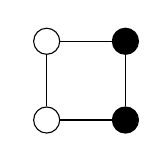
\begin{tikzpicture}
        \node[shape=circle,draw=black,fill=black] (A) at (1,0){};
        \node[shape=circle,draw=black,fill=black] (B) at (1,1){};
        \node[shape=circle,draw=black] (C) at (0,1){}; 
        \node[shape=circle,draw=black] (D) at (0,0){};
        \path [-](A) edge node[left]{} (B);
        \path [-](B) edge node[left]{} (C);
        \path [-](C) edge node[left]{} (D);
        \path [-](D) edge node[left]{} (A);
    \end{tikzpicture}
    \qquad
    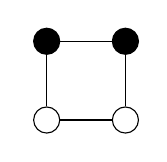
\begin{tikzpicture}
        \node[shape=circle,draw=black] (A) at (1,0) {};
        \node[shape=circle,draw=black,fill=black] (B) at (1,1) {};
        \node[shape=circle,draw=black,fill=black] (C) at (0,1) {};
        \node[shape=circle,draw=black] (D) at (0,0) {};
        \path [-](A) edge node[left]{} (B);
        \path [-](B) edge node[left]{} (C);
        \path [-](C) edge node[left]{} (D);
        \path [-](D) edge node[left]{} (A);
    \end{tikzpicture}
    \qquad
    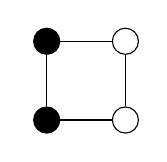
\begin{tikzpicture}
        \node[shape=circle,draw=black] (A) at (1,0) {};
        \node[shape=circle,draw=black] (B) at (1,1) {};
        \node[shape=circle,draw=black,fill=black] (C) at (0,1) {};
        \node[shape=circle,draw=black,fill=black] (D) at (0,0) {};
        \path [-](A) edge node[left]{} (B);
        \path [-](B) edge node[left]{} (C);
        \path [-](C) edge node[left]{} (D);
        \path [-](D) edge node[left]{} (A);
    \end{tikzpicture}
    \qquad
    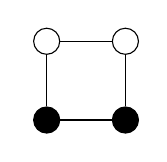
\begin{tikzpicture}
        \node[shape=circle,draw=black,fill=black] (A) at (1,0) {};
        \node[shape=circle,draw=black] (B) at (1,1) {};
        \node[shape=circle,draw=black] (C) at (0,1) {};
        \node[shape=circle,draw=black,fill=black] (D) at (0,0) {};
        \path [-](A) edge node[left]{} (B);
        \path [-](B) edge node[left]{} (C);
        \path [-](C) edge node[left]{} (D);
        \path [-](D) edge node[left]{} (A);
    \end{tikzpicture}
\end{equation}
will be considered as equivalent. Let $G=\langle g\rangle$ the cyclic 
group of order four. Let $X$ be 
the set of colorings of the square. Then 
$|X|=16$. 

Let $G$ acts on $X$ by anti-clockwise rotations  
of 90\textdegree. All the colorings of~\eqref{eq:orbita} belong to the same orbit. 
Another orbit of $X$ is
\[
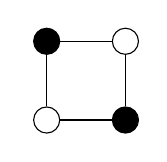
\begin{tikzpicture}
    \node[shape=circle,draw=black,fill=black] (A) at (1,0) {};
    \node[shape=circle,draw=black] (B) at (1,1) {};
    \node[shape=circle,draw=black,fill=black] (C) at (0,1) {};
    \node[shape=circle,draw=black] (D) at (0,0) {};
    \path [-](A) edge node[left]{} (B);
    \path [-](B) edge node[left]{} (C);
    \path [-](C) edge node[left]{} (D);
    \path [-](D) edge node[left]{} (A);
\end{tikzpicture}
\qquad
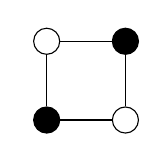
\begin{tikzpicture}
    \node[shape=circle,draw=black] (A) at (1,0) {};
    \node[shape=circle,draw=black,fill=black] (B) at (1,1) {};
    \node[shape=circle,draw=black] (C) at (0,1) {};
    \node[shape=circle,draw=black,fill=black] (D) at (0,0) {};
    \path [-](A) edge node[left]{} (B);
    \path [-](B) edge node[left]{} (C);
    \path [-](C) edge node[left]{} (D);
    \path [-](D) edge node[left]{} (A);
\end{tikzpicture}
\]

Cauchy--Frobenius--Burnside's theorem states that
there are  
\[
\frac{1}{|G|}\sum_{x\in G}|\Fix(x)|
\]
orbits. 

For each $x\in G=\{1,g,g^2,g^3\}$ we compute $\Fix(x)$. The identity fixes 
the 16 elements of $X$, both 
$g$ and  $g^3$ fix only two elements of $X$ and 
$g^2$ fixes four elements of $X$. For example, 
the elements of $X$ fixed by $g^2$ are 
\[
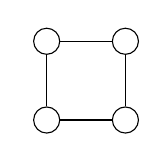
\begin{tikzpicture}
    \node[shape=circle,draw=black] (A) at (1,0){};
    \node[shape=circle,draw=black] (B) at (1,1){};
    \node[shape=circle,draw=black] (C) at (0,1){}; 
    \node[shape=circle,draw=black] (D) at (0,0){};
    \path [-](A) edge node[left]{} (B);
    \path [-](B) edge node[left]{} (C);
    \path [-](C) edge node[left]{} (D);
    \path [-](D) edge node[left]{} (A);
\end{tikzpicture}
\qquad
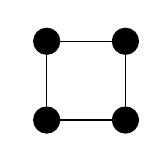
\begin{tikzpicture}
    \node[shape=circle,draw=black,fill=black] (A) at (1,0) {};
    \node[shape=circle,draw=black,fill=black] (B) at (1,1) {};
    \node[shape=circle,draw=black,fill=black] (C) at (0,1) {};
    \node[shape=circle,draw=black,fill=black] (D) at (0,0) {};
    \path [-](A) edge node[left]{} (B);
    \path [-](B) edge node[left]{} (C);
    \path [-](C) edge node[left]{} (D);
    \path [-](D) edge node[left]{} (A);
\end{tikzpicture}
\qquad
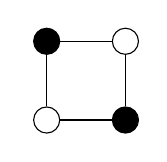
\begin{tikzpicture}
    \node[shape=circle,draw=black,fill=black] (A) at (1,0) {};
    \node[shape=circle,draw=black] (B) at (1,1) {};
    \node[shape=circle,draw=black,fill=black] (C) at (0,1) {};
    \node[shape=circle,draw=black] (D) at (0,0) {};
    \path [-](A) edge node[left]{} (B);
    \path [-](B) edge node[left]{} (C);
    \path [-](C) edge node[left]{} (D);
    \path [-](D) edge node[left]{} (A);
\end{tikzpicture}
\qquad
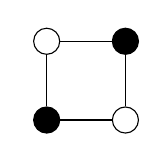
\begin{tikzpicture}
    \node[shape=circle,draw=black] (A) at (1,0) {};
    \node[shape=circle,draw=black,fill=black] (B) at (1,1) {};
    \node[shape=circle,draw=black] (C) at (0,1) {};
    \node[shape=circle,draw=black,fill=black] (D) at (0,0) {};
    \path [-](A) edge node[left]{} (B);
    \path [-](B) edge node[left]{} (C);
    \path [-](C) edge node[left]{} (D);
    \path [-](D) edge node[left]{} (A);
\end{tikzpicture}
\]
Thus $X$ is union of  
\[
\frac{1}{|G|}\sum_{x\in G}|\Fix(x)|=\frac{1}{4}(16+2+4+2)=6
\]
orbits. 
\end{example}

\begin{exercise}
    In how many ways (up to symmetry) can you
    arrange eight non-attacking rooks on a chessboard? Symmetries 
    are given by the dihedral group $\D_4$ of eight elements.
\end{exercise}

For a finite group $G$ let $\cp(G)$ be the probability 
that two random elements of $G$ commute. 
As an application of Cauchy--Frobenius--Burnside's theorem we
prove that 
$\cp(G)=k/|G|$, where $k$ is the number of conjugacy classes
of $G$.

\begin{theorem}
\index{Theorem!5/8}
\index{Erd\"os--Turan's theorem}
    If $G$ is a non-abelian finite group, then $\cp(G)\leq5/8$.
\end{theorem}

\begin{proof}
    Let $C=\{(x,y)\in G\times G:xy=yx\}$. We claim that  
    \[
    \cp(G)=\frac{|C|}{|G|^2}=\frac{k}{|G|}.
    \]
    In fact, let $G$ act on $G$ by conjugation. 
    By Cauchy--Frobenius--Burnside's theorem, 
    \[
    k=\frac{1}{|G|}\sum_{g\in G}|\Fix(g)|=\frac{1}{|G|}\sum_{g\in G}|C_G(g)|=\frac{|C|}{|G|},
    \]
    as $\Fix(g)=\{x\in G:gxg^{-1}=x\}=C_G(g)$ and $\sum_{g\in G}|C_G(g)|=|C|$. 

    We now claim that $k/|G|\leq 5/8$ if $G$ is non-abelian.
    
    Let $y_1,\dots,y_m$ the representatives of conjugacy classes of $G$ 
    of size $\geq2$. By the class equation, 
    \[
    |G|=|Z(G)|+\sum_{i=1}^m(G:C_G(y_i))\geq |Z(G)|+2m.
    \]
    Thus $m\leq(1/2)(|G|-|Z(G)|)$ and hence 
    \[
    k=|Z(G)|+m\leq |Z(G)|+\frac12(|G|-|Z(G)|)=\frac12(|Z(G)|+|G|).
    \]
    Since $G$ is non-abelian, $G/Z(G)$ is not cyclic. In particular, 
    $(G:Z(G))\geq4$. Therefore
    \[
    k\leq\frac12(|Z(G)|+|G|)\leq\frac12\left(\frac14+1\right)|G|,
    \]
    that is $k/|G|\leq 5/8$. 
\end{proof}

\begin{exercise}
    Prove that $\cp(Q_8)=5/8$. 
\end{exercise}

\begin{exercise}
    Let $G$ be a finite non-abelian group and $p$ be the smallest prime number
    dividing $|G|$. Prove that $\cp(G)\leq (p^2+p-1)/p^3$. Moreover, 
    the equality holds if and only if $(G:Z(G))=p^2$. 
\end{exercise}

\begin{exercise}
    Let $G$ be a finite group and $H$ be a subgroup of $G$.
    \begin{enumerate}
        \item $\cp(G)\leq\cp(H)$.
        \item If $H$ is normal in $G$, then $\cp(G)\leq\cp(G/H)\cp(H)$.
    \end{enumerate}
\end{exercise}

Degrees of irreducible characters give a lower bound:

\begin{proposition}
If $G$ is a finite group, then
\[
\cp(G)\geq\left(\frac{\sum_{\chi\in\Irr(G)}\chi(1)}{|G|}\right)^2.
\]
\end{proposition}

\begin{proof}
    Let $k$ be the number of conjugacy classes of $G$.
    By Cauchy--Schwarz's inequality, 
    \begin{align*}
        \left(\sum_{\chi\in\Irr(G)}\chi(1)\right)^2
        &\leq\left(\sum_{\chi\in\Irr(G)}\chi(1)^2\right)\left(\sum_{\chi\in\Irr(G)}1\right)^2
        =\left(\sum_{\chi\in\Irr(G)}\chi(1)^2\right)k=|G|k.
    \end{align*}
    From this the claim follows.
\end{proof}

\begin{theorem}[Dixon]
    \index{Dixon's theorem}
    If $G$ is a finite simple group, then $\cp(G)\leq1/12$.
\end{theorem}

The theorem appeared in 1970, as a problem in 
volume 13 of the \emph{Canadian Math. Bulletin}. The solution
appeared in 1973. 

\begin{exercise}
    Prove that $\cp(\Alt_5)=1/12$. 
\end{exercise}

The alternating group $\Alt_5$ is important in this setting:

\begin{theorem}[Guralnick--Robinson]
    \index{Guralnick--Robinson's theorem}
    If $G$ is a finite non-solvable group such that $\cp(G)>3/40$, then
    $G\simeq\Alt_5\times T$ for some abelian group 
    $T$ and $\cp(G)=1/12$. 
\end{theorem}

The proof appears in~\cite{MR2228209}.

Results on probability of commuting elements generalize in other directions. 
In~\cite{MR230809,MR276325,MR313378,MR369512}, 
Thompson proved the following result:

\begin{theorem}[Thompson]
\index{Thompson's theorem}
    If $G$ is a finite group such that 
    every pair of elements of $G$ generate
    a solvable group, then $G$ is solvable. 
\end{theorem}

The proof uses the classification of finite simple groups (CFSG). A simpler
proof independent of the CFSG appears in~\cite{MR1346207}.

There is a probabilistic version of Thompson's theorem:

\begin{theorem}[Guralnick--Wilson]
    \index{Guralnick--Wilson's theorem}
    Let $G$ be a finite group.
    \begin{enumerate}
        \item If the probability that two random elements of $G$ 
        generate a solvable group is $>11/30$, then $G$ is solvable. 
        \item If the probability that two random elements of $G$ 
        generate a nilpotent group is $>1/2$, then $G$ is nilpotent.
        \item If the probability that two random elements of $G$ 
        generate a group of odd order is $>11/30$, then $G$ has odd order.
    \end{enumerate}
\end{theorem}

The proof uses the CFSG and appears in~\cite{MR1770615}.



Nos basaremos en~\cite{MR1997347} y veremos otras aplicaciones del teorema de Cauchy--Frobenius--Burnside. 

\begin{theorem}[Jordan]
\index{Teorema!de Jordan}
Sea $G$ un grupo finito no trivial. Si $G$ actúa transitivamente en un conjunto finito $X$ y $|X|>1$, entonces
existe $g\in G$ sin puntos fijos. 
\end{theorem}

\begin{proof}
El teorema de Cauchy--Frobenius--Burnside implica que
\[
1=\frac{1}{|G|}\sum_{g\in G}|\Fix(g)|=\frac{1}{|G|}\left(|X|+\sum_{g\ne 1}|\Fix(g)|\right).
\]
Si todo $g\in G\setminus\{1\}$ contiene al menos un punto fijo, entonces
\[
1=\frac{1}{|G|}\left(|X|+\sum_{g\ne 1}|\Fix(g)|\right)\geq \frac{1}{|G|}(|X|+|G|-1)=1+\frac{|X|-1}{|G|}
\]
y luego $|X|\leq1$, una contradicción. 
\end{proof}

\begin{corollary}
Sea $G$ un grupo finito y $H$ un subgrupo propio de $G$. Entonces $G\ne\cup_{g\in G}gHg^{-1}$.
\end{corollary}

\begin{proof}
El grupo $G$ actúa transitivamente en $X=G/H$ por multiplicación a izquierda. 
El estabilizador de $xH$ es 
\[
G_{xH}=\{g\in G:gxH=xH\}=xHx^{-1}.
\]
Como $H\ne G$, entonces $|X|=|G/H|>1$. El teorema de Jordan implica entonces que existe $g\in G$ sin puntos fijos, es decir
que existe $g\in G$ tal que $g\not\in\cup_{x\in G}xHx^{-1}$. 
\end{proof}

Sea $G$ un grupo finito. Diremos que dos clases de conjugación $C$ y $D$ \textbf{conmutan} si existen 
$c\in C$ y $d\in D$ tales que $[c,d]=1$. 
Observemos que $C$ y $D$ conmutan si y sólo si para todo $c\in C$ existe $d\in D$ tal que $[c,d]=1$. 

\begin{corollary}[Wildon]
\index{Teorema!de Wildon}
    Sea $G$ un grupo finito y sea $C$ una clase de conjugación de $G$. Entonces
    $|C|=1$ si y sólo si $C$ conmuta con cualquier clase de conjugación de $G$. 
\end{corollary}
    
\begin{proof}
    Si $C=\{c\}$, entonces $c\in Z(G)$ y luego $C$ conmuta con cualquier clase de conjugación de $G$. Recíprocamente, supongamos que 
    $C$ conmuta con cualquier clase de conjugación de $G$. Si $c\in C$ y $H=C_G(c)$, entonces $H\cap D\ne\emptyset$ para toda
    clase de conjugación $D$. Afirmamos que entonces $G=\cup_{g\in G}gHg^{-1}$. En efecto, sea $x\in G$. Entonces $x\in D$ 
    para alguna clase de conjugación $D$. 
    Sea 
    $h\in H\cap D$. Existe $y\in G$ tal que $h=yxy^{-1}$, es decir $x=y^{-1}hy\in \cup_{g\in G}gHg^{-1}$. Por el teorema de Jordan, 
    $H=G$. Luego $c$ es central, es decir $C=\{c\}$. 
\end{proof}

La clasificación de grupos simples finitos permite demostrar un teorema
similar al teorema de Jordan~\cite{MR636194}. 

\begin{theorem}[Fein--Kantor--Schacher]
\index{Teorema!de Fein--Kantor--Schacher}
Sea $G$ un grupo finito no trivial. Si $G$ actúa transitivamente en un conjunto finito $X$ y $|X|>1$, entonces
existe un primo $p$ y un elemento $g\in G$ sin puntos fijos cuyo orden es una potencia de $p$. 
%existe $g\in G$ de orden una potencia de $p$ sin puntos fijos. 
\end{theorem}

No veremos la demostración en este curso. 

\index{Desarreglos}
Supongamos que $G$ es un grupo finito que actúa fiel y transitivamente en un conjunto $X$,
digamos $G\leq\Sym_n$, donde $X=\{1,2,\dots,n\}$. Sea 
$G_0$ el conjunto de $g\in G$ sin puntos fijos, es decir $g(x)\ne x$ para todo $x\in X$. 
Tales permutaciones se conocen como \textbf{desarreglos}. 
Sea $c_0=|G_0|/|G|$. 

\begin{theorem}[Cameron--Cohen]
\index{Teorema!de Cameron--Cohen}
Si $G$ es un subgrupo de $\Sym_n$ que actúa transitivamente en $\{1,\dots,n\}$, entonces $c_0\geq\frac{1}{n}$.
\end{theorem}

\begin{proof}
Sea $X=\{1,\dots,n\}$. El rango de $G$ es, por definición, la cantidad de orbitales de $G$ en $X$. Luego 
el rango de $G$ es $\geq2$, pues $X\times X$ puede descomponerse como 
$X\times X=\Delta\cup\left((X\times X)\setminus\Delta\right)$. 
Sean $\chi(g)=|\Fix(g)|$ y $G_0=\{g\in G:\chi(g)=0\}$. Si $g\not\in G_0$, entonces $1\leq\chi(g)\leq n$. Como 
$(\chi(g)-1)(\chi(g)-n)\leq 0$,
se tiene que 
\[
\frac{1}{|G|}\sum_{g\in G\setminus G_0}(\chi(g)-1)(\chi(g)-n)\leq 0.
\]
Por un lado, 
\begin{align*}
\frac{1}{|G|}\sum_{g\in G}(\chi(g)&-1)(\chi(g)-n)\\
&=\frac{1}{|G|}\left\{\sum_{g\in G_0}+\sum_{g\in G\setminus G_0}\right\}(\chi(g)-1)(\chi(g)-n)\\
&\leq n\frac{|G_0|}{|G|}=nc_0.
\end{align*}
Por otro lado, como el rango de $G$ es $\geq2$, tenemos 
\begin{equation}
    \label{eq:CameronCohen}
    2-\frac{n+1}{|G|}\sum_{g\in G}\chi(g)+n\leq 
    \frac{1}{|G|}\sum_{g\in G}(\chi(g)-1)(\chi(g)-n)\leq nc_0.
\end{equation}
Por hipotesis, $G$ es transitivo en $X$. El teorema de Cauchy--Frobenius--Burnside implica entonces que 
$\sum_{g\in G}\chi(g)=|G|$. Se sigue que $2-(n+1)+n\leq nc_0$ y luego $1/n\leq c_0$. 
% Si $c_0=1/n$, entonces $G$ tiene rango dos (pues si el rango de $G$ es $>2$ entonces la fórmula~\eqref{eq:CameronCohen}
% implica que $1/n<c_0$). Además, por un lado, 
% \begin{align*}
% \frac{1}{|G|}\sum_{g\in G}(\chi(g)-1)(\chi(g)-n)&=\frac{1}{|G|}\sum_{g\in G}\chi(g)^2-\frac{n+1}{|G|}\sum_{g\in G}\chi(g)+n\\
% &=2-(n+1)+n=1.    
% \end{align*}
% Por otro lado, como $c_0=|G_0|/|G|=1/n$, 
% \begin{align*}
% \frac{1}{|G|}\sum_{g\in G}(\chi(g)-1)(\chi(g)-n)
% &=\frac{1}{|G|}\sum_{g\in G\setminus G_0}(\chi(g)-1)(\chi(g)-n)\\
% &=\frac{1}{|G|}\sum_{g\in G_0}(\chi(g)-1)(\chi(g)-n)\\
% &=\frac{1}{|G|}\sum_{g\in G\setminus G_0}(\chi(g)-1)(\chi(g)-n)+1.
% \end{align*}
% Luego $\frac{1}{|G|}\sum_{g\in G\setminus G_0}(\chi(g)-1)(\chi(g)-n)=0$ y entonces $(\chi(g)-1)(\chi(g)-n)$ para todo $g\in G\setminus G_0$.
\end{proof}

El teorema de Cameron--Cohen tiene una segunda parte: 
Si $n$ no es potencia de un primo, entonces $c_0>1/n$. 
Daremos la demostración en el capítulo~\ref{Frobenius}, donde 
estudiaremos grupos de Frobenius.  

La cota del teorema de Cameron--Cohen puede mejorarse si se utiliza la 
clasificación de grupos simples finitos~\cite{MR1484879}.  

\begin{theorem}[Guralnick--Wan]
\index{Teorema!de Guralnick--Wan}
Sea $G$ un grupo finito transitivo de grado $n\geq2$. Si $n$ no es potencia de un 
número primo 
y además $G\ne\Sym_n$ para $n\in\{2,4,5\}$, entonces $c_0\geq 2/n$.
\end{theorem}

La demostración utiliza la clasificación de grupos finitos 2-transitivos, que depende del 
la clasificación de grupos simples finitos.




\chapter{}

\topic{The correspondence theorem}

Let $N$ be a normal subgroup of $G$ 
and $\pi\colon G\to G/N$, $g\mapsto gN$, be the canonical map. 
If $\widetilde{\rho}\colon G/N\to\GL(V)$ 
is a representation of $G/N$ with 
character
$\widetilde{\chi}$, the composition 
$\rho=\widetilde{\rho}\pi\colon G\to \GL(V)$, $\rho(g)=\widetilde{\rho}(gN)$, 
is a representation of $G$. 
Thus
\[
\chi(g)=\trace{\rho_g}=\trace(\widetilde{\rho}_{gN})=\widetilde{\chi}(gN).
\]
In particular, $\chi(1)=\widetilde{\chi}(1)$. The character $\chi$ 
is the \textbf{lifting} to $G$ of the character 
$\widetilde{\chi}$ of $G/N$. 

\begin{proposition}
If $\chi\in\Char(G)$, then 
\[
\ker\chi=\{g\in G:\chi(g)=\chi(1)\}
\]
is a normal subgroup of $G$. 
\end{proposition}

\begin{proof}
Let $\rho\colon G\to\GL_n(\C)$ be a representation with character $\chi$. Then 
$\ker\rho\subseteq\ker\chi$, as $\rho_g=\id$ implies 
$\chi(g)=\trace(\rho_g)=n=\chi(1)$. We claim that  
$\ker\chi\subseteq\ker\rho$. If $g\in G$ is such that $\chi(g)=\chi(1)$, since 
$\rho_g$ is diagonalizable, there exist eigenvalues $\lambda_1,\dots,\lambda_n\in\C$ such that
\[
n=\chi(1)=\chi(g)=\sum_{i=1}^n\lambda_i.
\]
Since each $\lambda_i$ is a root of one,  
$\lambda_1=\cdots=\lambda_n=1$. Hence $\rho_g=\id$. 
\end{proof}

\index{Kernel!of a character}
If $\chi$ is a character, the subgroup $\ker\chi$ 
is the \textbf{kernel} of $\chi$. 

\begin{theorem}[Correspondence theorem]
\index{Correspondence theorem!for characters}
Let $N$ be a normal subgroup of a finite group $G$. There exists
a bijective correspondence 
\[
\Char(G/N) \longleftrightarrow \{\chi\in\Char(G): 
N\subseteq\ker\chi\}
\]
that maps irreducible characters to irreducible characters.
\end{theorem}

\begin{proof}
If $\widetilde{\chi}\in\Char(G/N)$, let $\chi$ be the lifting of $\widetilde{\chi}$ to $G$. If $n\in N$, 
then
\[
\chi(n)=\widetilde{\chi}(nN)=\widetilde{\chi}(N)=\chi(1)
\]
and thus $N\subseteq\ker\chi$. 

If $\chi\in\Char(G)$ is such that $N\subseteq\ker\chi$, let $\rho\colon G\to\GL(V)$ be a representation
with character $\chi$. 
Let $\widetilde{\rho}\colon G/N\to\GL(V)$, $gN\mapsto \rho(g)$. We claim that $\widetilde{\rho}$
is well-defined: 
\[
gN=hN\Longleftrightarrow h^{-1}g\in N\Longrightarrow\rho(h^{-1}g)=\id\Longleftrightarrow \rho(h)=\rho(g).
\]
Moreover, $\widetilde{\rho}$ is a representation, as 
\[
\widetilde{\rho}((gN)(hN))=\widetilde{\rho}(ghN)=\rho(gh)=\rho(g)\rho(h)=\widetilde{\rho}(gN)\widetilde{\rho}(hN).
\]
If $\widetilde{\chi}$ is the character of $\widetilde{\rho}$, then 
$\widetilde{\chi}(gN)=\chi(g)$.

We now prove that $\chi$ is irreducible if and only if 
$\widetilde{\chi}$ is irreducible. If $U$ is a subspace of $V$, then 
\begin{align*}
\text{$U$ is $G$-invariant}
%&\Longleftrightarrow g\cdot U\subseteq U\text{ for all $g\in G$}\\
&\Longleftrightarrow \rho(g)(U)\subseteq U\text{ for all $g\in G$}\\
&\Longleftrightarrow \widetilde{\rho}(gN)(U)\subseteq U\text{ for all $g\in G$}.
\shortintertext{Thus}
\chi\text{ is irreducible }&\Longleftrightarrow
\rho\text{ is irreducible }\\
&\Longleftrightarrow\widetilde{\rho}\text{ is irreducible }\Longleftrightarrow
\widetilde{\chi}\text{ is irreducible }\qedhere.
\end{align*}
\end{proof}

\begin{example}
    Let $G=\Sym_4$ and $N=\{\id,(12)(34),(13)(24),(14)(23)\}$. We know that $N$ is normal in $G$ 
    and that $G/N=\langle a,b\rangle\simeq\Sym_3$, where 
    $a=(123)N$ and $b=(12)N$. 
    The character table of $G/N$ is 
    \begin{center}
		\begin{tabular}{|c|rrr|}
			\hline
			%& $1$ & $3$ & $2$\tabularnewline
			& $N$ & $(12)N$ & $(123)N$ \tabularnewline
			\hline 
			$\widetilde{\chi}_{1}$ & $1$ & $1$ & $1$\tabularnewline
			$\widetilde{\chi}_{2}$ & $1$ & $-1$ & $1$ \tabularnewline
			$\widetilde{\chi}_{3}$ & $2$ & $0$ & $-1$ \tabularnewline
			\hline
		\end{tabular}
	\end{center}
    For each $i\in\{1,2,3\}$ we compute the lifting $\chi_i$ to $G$ of the character  
    $\widetilde{\chi}_i$ of $G/N$. 
    Since $(12)(34)\in N$ and $(13)(1234)=(12)(34)\in N$, 
    \begin{align*}
        \chi( (12)(34) )=\widetilde{\chi}(N),\quad
        \chi( (1234) )=\widetilde{\chi}((13)N)=\widetilde{\chi}((12)N).
    \end{align*}
    Since the characters $\widetilde{\chi_i}$ are irreducibles, 
    the liftings $\chi_i$ are also irreducibles. With this process
    we obtain the following irreducible characters of $G$:
    	\begin{center}
		\begin{tabular}{|c|rrrrr|}
			\hline
			& $1$ & $(12)$ & $(123)$ & $(12)(34)$ & $(1234)$ \tabularnewline
			\hline 
			$\chi_{1}$ & $1$ & $1$ & $1$ & 1 & 1\tabularnewline
			$\chi_{2}$ & $1$ & $-1$ & $1$ & 1 & -1 \tabularnewline
			$\chi_{3}$ & $2$ & $0$ & $-1$ & 2 & 0\tabularnewline
			\hline
		\end{tabular}
	\end{center}
\end{example}

The character table of a group can be used to find the lattice 
of normal subgroups. In particular, the character table detects simple groups. 

\begin{lemma}
    Let $G$ be a finite group and 
    let $g,h\in G$. Then $g$ and $h$ 
    are conjugate if and only if 
    $\chi(g)=\chi(h)$ for all
    $\chi\in\Char(G)$. 
\end{lemma}

\begin{proof}
    If $g$ and $h$ are conjugate, then $\chi(g)=\chi(h)$, as characters are class functions
    of $G$.
    Conversely, if $\chi(g)=\chi(h)$ for all $\chi\in\Char(G)$, then 
    $f(g)=f(h)$ for all class function $f$ of $G$, 
    as characters $G$ generate the space of class functions of $G$. In particular, 
    $\delta(g)=\delta(h)$, where
    \[
    \delta(x)=\begin{cases}
    1 & \text{if $x$ and $g$ are conjugate},\\
    0 & \text{otherwise}.
    \end{cases}
    \]
    This implies that $g$ and $h$ are conjugate.
\end{proof}

As a consequence, we get that 
\begin{equation}
\label{eq:kernels}
\bigcap_{\chi\in\Irr(G)}\ker\chi=\{1\}.
\end{equation}
Indeed, if $g\in\ker\chi$ for all $\chi\in\Irr(G)$, then $g=1$ since 
the lemma implies that $g$ and $1$ are conjugate
because 
$\chi(g)=\chi(1)$ for all $\chi\in\Irr(G)$.

\begin{proposition}
\label{pro:normal}
    Let $G$ be a finite group. 
    If $N$ is a normal subgroup of $G$, 
    then there exist characters
    $\chi_1,\dots,\chi_k\in\Irr(G)$ 
    such that
    \[
    N=\bigcap_{i=1}^k\ker\chi_i.
    \]
\end{proposition}

\begin{proof}
    Apply the previous remark to the group $G/N$ to obtain that 
    \[
    \bigcap_{\widetilde{\chi}\in\Irr(G/N)}\ker\widetilde{\chi}=\{N\}.
    \]
    Assume that $\Irr(G/N)=\{\widetilde{\chi}_1,\dots,\widetilde{\chi}_k\}$. 
    We lift the irreducible characters of $G/N$ to $G$ 
    to obtain (some) irreducible characters $\chi_1,\dots,\chi_k$ 
    of $G$ such that 
    \[
    N\subseteq\ker\chi_1\cap\cdots\cap\ker\chi_k.
    \]
    If $g\in\ker\chi_i$ for all $i\in\{1,\dots,k\}$, then 
    \[
    \widetilde{\chi}_i(N)=\chi_i(1)=\chi_i(g)=\widetilde{\chi}_i(gN)
    \]
    for all $i\in\{1,\dots,k\}$. This implies that
    \[
    gN\in\bigcap_{i=1}^k\ker\widetilde{\chi}_i=\{N\},
    \]
    that is $g\in N$. 
\end{proof}

\index{Group!simple}
Recall that a non-trivial group is \textbf{simple} if it contains no non-trivial normal 
proper subgroups. Examples of simple groups are cyclic groups of prime order
and the alternating groups $\Alt_n$ for $n\geq5$. 
As a corollary of Proposition \ref{pro:normal}, 
we can use the character table to detect simple groups.

\begin{proposition}
    Let $G$ be a finite group. Then $G$ is not simple if and only if 
    there exists a non-trivial irreducible character $\chi$ such that
    $\chi(g)=\chi(1)$ 
    for some $g\in G\setminus\{1\}$. 
\end{proposition}

\begin{proof}
    If $G$ is not simple, there exists a normal subgroup $N$ of $G$ such that
    $N\ne G$ and $N\ne\{1\}$. 
    By Proposition \ref{pro:normal}, there exist characters 
    $\chi_1,\dots,\chi_k\in\Irr(G)$
    such that 
    $N=\ker\chi_1\cap\cdots\cap\ker\chi_k$.
    In particular, there exists a non-trivial character
    $\chi_i$ such that $\ker\chi_i\ne\{1\}$. Thus 
    there exists $g\in G\setminus\{1\}$ such that
    $\chi_i(g)=\chi_i(1)$. 
    
    Assume now that there exists a non-trivial irreducible character $\chi$ 
    such that $\chi(g)=\chi(1)$ for some $g\in G\setminus\{1\}$. In particular, $g\in\ker\chi$ 
    and hence $\ker\chi\ne\{1\}$. Since $\chi$ is non-trivial, $\ker\chi\ne G$. 
    Thus $\ker\chi$ is a proper non-trivial normal subgroup of $G$.
\end{proof}

\begin{example}
\index{Mathieu's group $M_9$}
    If there exists a group $G$ with
    a character table 
    of the form
    \begin{center}
		\begin{tabular}{|c|rrrrrr|}
			\hline
			$\chi_{1}$ & 1 & 1 & 1 & 1 & 1 & 1\tabularnewline
			$\chi_{2}$ & 1 & 1 & 1 & -1 & 1 & -1 \tabularnewline
			$\chi_{3}$ & 1 & 1 & 1 & 1 & -1 & -1\tabularnewline
		    $\chi_{4}$ & 1 & 1 & 1 & -1 & -1 & 1\tabularnewline
			$\chi_{5}$ & 2 & -2 & 2 & 0 & 0 & 0\tabularnewline
			$\chi_{6}$ & 8 & 0 & -1 & 0 & 0 & 0\tabularnewline
			\hline
		\end{tabular}
	\end{center}
	then $G$ cannot be simple. Note that such a group $G$ would have order $\sum_{i=1}^6\chi_i(1)^2=72$. 
	Mathieu's group $M_{9}$ has precisely this character table! 
\end{example}

\begin{example}
    Let $\alpha=\frac{1}{2}(-1+\sqrt{7}i)$. 
    If there exists a group $G$ with a character table
    of the form
    \begin{center}
		\begin{tabular}{|c|rrrrrr|}
			\hline
			$\chi_{1}$ & 1 & 1 & 1 & 1 & 1 & 1\tabularnewline
			$\chi_{2}$ & 7 & -1 & -1 & 1 & 0 & 0 \tabularnewline
			$\chi_{3}$ & 8 & 0 & 0 & -1 & 1 & 1\tabularnewline
		    $\chi_{4}$ & 3 & -1 & 1 & 0 & $\alpha$ & $\overline{\alpha}$ \tabularnewline
			$\chi_{5}$ & 3 & -1 & 1 & 0 & $\overline{\alpha}$ & $\alpha$\tabularnewline
			$\chi_{6}$ & 6 & 2 & 0 & 0 & 0 & 0\tabularnewline
			\hline
		\end{tabular}
	\end{center}    
	then $G$ is simple. Note that such a group $G$ would have order 
	$\sum_{i=1}^6\chi_i(1)^2=168$. 
	The group  
	\[
	\PSL_2(7)=\SL_2(7)/Z(\SL_2(7))
	\]
	is a simple group that has precisely this character table!  
\end{example}

\topic{Frobenius' groups}
\label{Frobenius}

If $p$ is a prime number, then
the units $(\Z/p)^{\times}$ 
of $\Z/p$ form a multiplicative group. Moreover, 
$(\Z/p)^{\times}$ 
is cyclic of order $p-1$. 

Let 
\[
G=\left\{\begin{pmatrix}
x & y\\
0 & 1
\end{pmatrix}
:x\in(\Z/p)^\times,\,y\in\Z/p\right\}.
\]
Then $G$ is a group with the usual matrix multiplication
and $|G|=p(p-1)$. 
Let $p$ and $q$ be prime numbers such that $q$ divides $p-1$, 
$z\in\Z$ be an element of multiplicative order $q$ modulo $p$ 
and 
\[
a=\begin{pmatrix}
1&1\\
0&1
\end{pmatrix},
\quad
b=\begin{pmatrix}
z&1\\
0&1
\end{pmatrix},
\quad
H=\langle a,b\rangle.
\]
A direct calculation shows that 
\begin{equation}
\label{eq:pq}
a^p=b^q=\begin{pmatrix}
1&0\\
0&1
\end{pmatrix},
\quad
bab^{-1}=\begin{pmatrix}
1&z\\
0&1
\end{pmatrix}
=a^z.
\end{equation}
Every element of $H$ is of the form $a^ib^j$ for $i\in\{0,\dots,p-1\}$ and  $j\in\{0,\dots,q-1\}$. 
Thus $|H|=pq$. Using~\eqref{eq:pq} we can compute 
the multiplication table of $G$. 

\begin{exercise}
    Let $p$ and $q$ be prime numbers such that $q$ divides $p-1$. Let
    $u,v\in\Z$ be elements of order $q$ modulo $p$. 
    Prove that 
    \[
    \langle a,b:a^p=b^q=1,bab=a^u\rangle
    \simeq \langle a,b:a^p=b^q=1,bab=a^v\rangle.
    \]
\end{exercise}

The group   
\[
F_{p,q}=\langle a,b:a^p=b^q=1,bab=a^u\rangle,
\]
where $u\in\Z$ has order $q$ modulo $p$, 
is a particular case of a  
\emph{Frobenius group}. 

\begin{proposition}
    Let $p$ and $q$ be prime numbers such that $p>q$. Let  
    $G$ be a group of order $pq$. Then either $G$ is abelian or
    $q$ divides $p-1$ and 
    $G\simeq F_{p,q}$.
\end{proposition}

\begin{proof}
    Assume that $G$ is not abelian. By Sylow's theorems, 
    $q$ divides $p-1$ and there exists 
    a unique Sylow $p$-subgroup $P$ of $G$. Let $a,b\in G$ be such that 
    $P=\langle a\rangle\simeq\Z/p$ and $G/P=\langle bP\rangle\simeq\Z/q$. By Lagrange's theorem, 
    $G=\langle a,b\rangle$. We compute the order of $b^q$. Since 
    $G$ is not cyclic (because it is not abelian) and $b^q\in P$, 
    we conclude that $|b^q|=1$. 
    Since $P$ is normal in $G$, 
    $bab^{-1}\in P$ and hence $bab^{-1}=a^z$ for some $z\in\Z$. Therefore
    $b^qab^{-q}=a^{z^q}$. This implies that 
    $z^q\equiv1\bmod p$. The order of $z$ in $(\Z/p)^{\times}$ divides 
    $q$ and hence it is equal to $q$ (otherwise, $z=1$ and thus $bab^{-1}=a$, which implies
    that $G$ is abelian). In conclusion, 
    $G\simeq F_{p,q}$. 
\end{proof}

With the proposition, we prove, for example, that 
every group of order 15 is abelian. We can also prove
that up to isomorphism $\Z/20$ and  
$F_{5,4}$ are the only groups of order 20. 

\begin{definition}
  \index{Frobenius!complement}
  \index{Frobenius!kernel}
  \index{Frobenius!group}
  We say that a finite group $G$ is a 
  \textbf{Frobenius group} if $G$ 
  has a non-trivial proper subgroup $H$ such that $H\cap
  xHx^{-1}=\{1\}$ for all $x\in G\setminus H$. In this case, the subgroup 
  $H$ is called a \textbf{Frobenius complement}.
\end{definition}

\begin{theorem}[Frobenius]
  \label{thm:Frobenius}
  \index{Frobenius'!theorem}
  Let $G$ be a Frobenius group with complement $H$. Then
  \[
	N=\left( G\setminus\bigcup_{x\in G}xHx^{-1}\right)\cup\{1\}
  \]
  is a normal subgroup of $G$.
\end{theorem}

\begin{proof}
  For each $\chi\in\Irr(H)$, $\chi\ne1_H$, let 
  $\alpha=\chi-\chi(1)1_H\in\cf(H)$, where $1_H$ denotes the trivial character of $H$. 

  We claim that $\Res_H^G\Ind_H^G\alpha=\alpha$.
  First, $\Ind_H^G\alpha(1)=\alpha(1)=0$. If $h\in H\setminus\{1\}$, then 
  \[
    \Ind_H^G\alpha(h)=\frac{1}{|H|}\sum_{\substack{x\in G\\x^{-1}hx\in H}}\alpha(x^{-1}hx)
    =\frac{1}{|H|}\sum_{x\in H}\alpha(h)=\alpha(h),
  \]
  since, if $x\not\in H$, then $x^{-1}hx\in H$ implies that 
  $h\in H\cap xHx^{-1}=\{1\}$.

  By Frobenius' reciprocity, 
  \begin{equation}
    \label{eq:<a,a>=1+chi2}
    \langle\Ind_H^G\alpha,\Ind_H^G\alpha\rangle
    =\langle\alpha,\Res_H^G\Ind_H^G\alpha\rangle=\langle\alpha,\alpha\rangle
    =1+\chi(1)^2.
  \end{equation}
  Again, by Frobenius' reciprocity, 
  \[
  \langle\Ind_H^G\alpha,1_G\rangle
  =\langle\alpha,\Res_H^G1_G\rangle
  =\langle\alpha,1_H\rangle
  =\langle\chi-\chi(1)1_H,1_H\rangle
  =-\chi(1),
  \]
  where $1_G$ is the trivial character of $G$. If we write 
  \[
  \Ind_H^G\alpha=\sum_{\eta\in\Irr(G)}\langle\Ind_H^G\alpha,\eta\rangle\eta
  =\langle\Ind_H^G\alpha,1_G\rangle1_G+\underbrace{\sum_{\substack{1_G\ne\eta\\\eta\in\Irr(G)}}\langle\Ind_H^G\alpha,\eta\rangle\eta}_{\phi},
  \]
  then $\Ind_H^G\alpha=-\chi(1)1_G+\phi$, where $\phi$ is a linear combination of non-trivial 
  irreducible characters of $G$. We compute 
  \[
  1+\chi(1)^2=\langle\Ind_H^G\alpha,\Ind_H^G\alpha\rangle
  =\langle\phi-\chi(1)1_G,\phi-\chi(1)1_G\rangle
  =\langle\phi,\phi\rangle+\chi(1)^2
  \]
  and hence $\langle\phi,\phi\rangle=1$. 
  
  \begin{claim}
  If $\eta\in\Irr(G)$ is such that $\eta\ne 1_G$, then 
  $\langle\Ind_H^G\alpha,\eta\rangle\in\Z$. 
  \end{claim}
  
  By Frobenius' reciprocity, $\langle\Ind_H^G\alpha,\eta\rangle=\langle\alpha,\Res_H^G\eta\rangle$. 
  If we decompose $\Res_H^G\eta$ into irreducibles of $H$, say 
  \[
  \Res_H^G\eta=m_11_H+m_2\chi+m_3\theta_3+\cdots+m_t\theta_t
  \]
  for some $m_1,m_2,\dots,m_t\geq0$, 
  then, since 
  \begin{align*}
  \langle\alpha,1_H\rangle=\langle\chi-\chi(1)1_H,1_H\rangle=-\chi(1),
  &&\langle\alpha,\chi\rangle=\langle\chi-\chi(1)1_H,\chi\rangle=1,
  \end{align*}
  and 
  \[
  \langle\alpha,\theta_j\rangle=\langle\chi-\chi(1)1_H,\theta_j\rangle=0
  \]
  for all $j\in\{3,\dots,t\}$, we conclude that 
  \[
  \langle\Ind_H^G\alpha,\eta\rangle=-m_1\chi(1)+m_2\in\Z.
  \]
  
  \begin{claim}
  $\phi\in\Irr(G)$.
  \end{claim}
  
  Since $\langle\Ind_H^G\alpha,\eta\rangle\in\Z$ for all $\eta\in\Irr(G)$ such that 
  $\eta\ne 1_G$ and 
  \[
  1=\langle\phi,\phi\rangle
  =\sum_{\substack{\eta,\theta\in\Irr(G)\\\eta,\theta\ne1_G}}\langle\Ind_H^G\alpha,\eta\rangle\langle\Ind_H^G\alpha,\theta\rangle\langle\eta,\theta\rangle
  =\sum_{\substack{\eta\ne 1_G\\\eta\in\Irr(G)}}\langle\Ind_H^G\alpha,\eta\rangle^2,
  \]
  there is a unique $\eta\in\Irr(G)$ such that 
  $\langle\Ind_H^G\alpha,\eta\rangle^2=1$ and all the other products are zero, 
  that is 
  $\phi=\pm\eta$ for some $\eta\in\Irr(G)$. Since 
  \[
  \chi-\chi(1)1_H=\alpha=\Res_H^G\Ind_H^G\alpha=\Res_H^G(\phi-\chi(1)1_G)=\Res_H^G\phi-\chi(1)1_H,
  \]
  it follows that $\phi(1)=\Res_H^G\phi(1)=\chi(1)\in\Z_{\geq1}$. Thus $\phi\in\Irr(G)$. 

  \medskip
  We have proved that if $\chi\in\Irr(H)$ is such that $\chi\ne 1_H$, then 
  there exists $\phi_\chi\in\Irr(G)$ such that $\Res_H^G(\phi_\chi)=\chi$. 
  
  \medskip
  We prove that $N$ is equal to 
  \[
	M=\bigcap_{\substack{\chi\in\Irr(H)\\\chi\ne1_H}}\ker\phi_{\chi}.
  \]

  We first prove that $N\subseteq M$. 
  Let $n\in N\setminus\{1\}$ and $\chi\in\Irr(H)\setminus\{1_H\}$. Since $n$ 
  does not belong to a conjugate of 
  $H$, 
  \[
	\Ind_H^G\alpha(n)=\frac{1}{|H|}\sum_{\substack{x\in G\\x^{-1}nx\in H}}\chi(x^{-1}nx)=0, 
  \]
  as $n\in N$ implies that the set $\{x\in G:x^{-1}nx\in H\}$ is empty. Since 
  \[
  0=\Ind_H^G\alpha(n)
  =\phi_{\chi}(n)-\chi(1)=\phi_{\chi}(n)-\phi_{\chi}(1),
  \]
  we conclude that $n\in\ker\phi_{\chi}$. 
  
  We now prove that $M\subseteq N$. 
  Let $h\in M\cap H$ and $\chi\in\Irr(H)\setminus\{1_H\}$. Then 
  \[
    \phi_{\chi}(h)-\chi(1)=\Ind_H^G\alpha(h)=\alpha(h)=\chi(h)-\chi(1),
  \]
  and $h\in\ker\chi$, as
  \[
    \chi(h)=\phi_{\chi}(h)=\phi_{\chi}(1)=\chi(1).
  \]
  Therefore $h\in\cap_{\chi\in\Irr(H)}\ker\chi=\{1\}$. By~\eqref{eq:kernels}, the kernels
  of irreducible characters have trivial intersection. 
  We now prove that $M\cap
  xHx^{-1}=\{1\}$ for all $x\in G$. Let $x\in G$ and $m\in M\cap xHx^{-1}$. Since 
  $m=xhx^{-1}$ for some $h\in H$, $x^{-1}mx\in H\cap M=\{1\}$.  This implies that 
  $m=1$.
\end{proof}

At the moment, there is no proof of Frobenius' theorem essentially 
independent of character theory. 

\begin{definition}
  \index{Frobenius!kernel}
  Let $G$ be a Frobenius group. The normal subgroup 
  $N$ of Frobenius' theorem is called the \textbf{Frobenius kernel}. 
\end{definition}

\begin{corollary}
  Let $G$ be a Frobenius group with complement $H$. 
  Then there exists a normal subgroup $N$ of $G$ 
  such that 
  $G=HN$ and $H\cap N=\{1\}$.
\end{corollary}

\begin{proof}
  Frobenius' theorem yields the subgroup $N$. 
  Let us prove that $H\supseteq N_G(H)$. If $h\in
  H\setminus\{1\}$ and $g\in G$ are such that $ghg^{-1}\in H$, then $h\in
  g^{-1}Hg\cap H$ and hence $g\in H$. Since $H=N_G(H)$, the subgroup $H$
  has $(G:H)$ conjugates. Thus $|G|=|H||N|$,
  where $N=\left( G\setminus\bigcup_{x\in G}xHx^{-1}\right)\cup\{1\}$, as 
  \[
    |N|=|G|-(G:H)(|H|-1)=(G:H).
  \]
  Since $N\cap H=\{1\}$, 
  \[
  |HN|=|N||H|/|H\cap N|=|N||H|=|G|
  \]
  and therefore $G=NH$.
\end{proof}

\subsection*{Some comments}

\begin{corollary}[Combinatorial Frobenius' theorem]
    \label{cor:Frobenius_combinatorio}
    \index{Frobenius'!theorem}
    Let $G$ be a group acting transitively on a finite set $X$. 
    Assume that each $g\in G\setminus\{1\}$ fixes 
    at most one element of 
     $X$. The set $N$ formed by the identity and 
     the permutations that move every element of $X$
     is a subgroup of $G$.
\end{corollary}

\begin{proof}
  Let $x\in X$ and $H=G_x$. We claim that 
  if $g\in G\setminus H$, then $H\cap
  gHg^{-1}=1$. If $h\in H\cap gHg^{-1}$, then
  $h\cdot x=x$ and $g^{-1}hg\cdot
  x=x$. Since $g\cdot x\ne x$, $h$ fixes two elements of
  $X$. Thus 
  $h=1$, as every non-trivial element fixes at most one element of $X$). 

  By Theorem~\ref{thm:Frobenius}, 
  \[
    N=\left(G\setminus\bigcup_{g\in G}gHg^{-1}\right)\cup\{1\}
  \]
  is a subgroup of $G$. Let us compute the elements of $N$. If 
  $h\in\cup_{g\in G}gHg^{-1}$, then there exists  $g\in G$ such that $g^{-1}hg\in H$,
  that is $(g^{-1}hg)\cdot x=x$; equivalently, 
  $h\in G_{g\cdot x}$. Therefore, the 
  non-identity elements of $N$ are the elements of $G$
  moving every element of $X$.
\end{proof}

\begin{example}
  Let $F$ be a finite field and $G$ be the group of maps 
  $f\colon F\to F$ of the form 
  $f(x)=ax+b$, $a,b\in F$ with $a\ne0$. The group $G$ acts on 
  $F$ and every 
  $f\ne\id$ fixes at most one element of $F$, as 
  \[
	x=f(x)=ax+b\implies a\ne 1\text{ and } x=b/(1-a).
  \]
  In this case, $N=\{f:f(x)=x+b\,,b\in F\}$ 
  is a subgroup of $G$.
\end{example}

\begin{exercise}
    Prove that Theorem~\ref{thm:Frobenius} can be obtained from
    Corollary~\ref{cor:Frobenius_combinatorio}.
\end{exercise}


% Wielandt 8.5.4
% 8.5.6 para ver algo de grupos de permutaciones
% 7.1 para ejemplo H(q)
% 10.5.6 (Thompson) N es nilpotente, se usa 10.5.4 

In his doctoral thesis Thompson proved the following result, conjectured
by Frobenius. 

\begin{theorem}[Thompson]
\index{Thompson's theorem}
    Let $G$ be a Frobenius group. If $N$ is the Frobenius kernel, then $N$ 
    is nilpotent.
\end{theorem}

See~\cite[Theorem 6.24]{MR2426855} for the proof.





\section{}

\subsection{Some theorems of Burnside}

For $n\geq1$ let $\{e_1,\dots,e_n\}$ be the standard basis of $\C^n$.  
The \emph{natural representation} of $\Sym_n$ is 
$\rho\colon\Sym_n\to\GL_n(C)$, $\sigma\mapsto\rho_{\sigma}$, 
where $\rho_\sigma(e_j)=e_{\sigma(j)}$ for all $j\in\{1,\dots,n\}$. 
The matrix of $\rho_\sigma$ in the standard basis is  
\begin{equation}
    \label{eq:Sn_natural}
    (\rho_\sigma)_{ij}=\begin{cases}
      1 & \text{if $i=\sigma(j)$},\\
      0 & \text{otherwise}.
    \end{cases}
\end{equation}

\begin{lemma}
	\label{lem:permutaciones}
	For $n\geq1$ let $\rho\colon\Sym_n\to\GL_n(C)$ be the natural 
	representation of the symmetric group. 
	If $A\in\C^{n\times n}$ and $\sigma\in\Sym_n$, then
	\[
		A_{ij}=(\rho_{\sigma}A)_{\sigma(i)j}=(A\rho_{\sigma})_{i\sigma^{-1}(j)}
	\]
    for all $i,j\in\{1,\dots,n\}$.
\end{lemma}

\begin{proof}
	With~\eqref{eq:Sn_natural} we compute:
	\[
		(A\rho_{\sigma})_{ij}=\sum_{k=1}^n A_{ik}(\rho_{\sigma})_{kj}=A_{i\sigma(j)},
		\quad
		(\rho_\sigma A)_{ij}=\sum_{k=1}^n (\rho_\sigma)_{ik}A_{kj}=A_{\sigma^{-1}(i)j}.\qedhere
	\]
\end{proof}

\begin{definition}
  \index{Real!character}
  Let $G$ be a finite group. A character $\chi$ of $G$ is said to be
  \emph{real} if
  $\chi=\overline{\chi}$, that is $\chi(g)\in\R$ for all $g\in G$. 
\end{definition}

\begin{exercise}
	\label{xca:chi_irreducible}
	Let $G$ be a finite group. If $\chi\in\Irr(G)$, then 
	$\overline{\chi}$ is irreducible.
\end{exercise}

\begin{definition}
  \index{Real!conjugacy class}
  Let $G$ be a group. A conjugacy class $C$ of $G$ is said to be
  \emph{real} if for every $g\in C$ one has $g^{-1}\in C$. 
\end{definition}

We use the following notation: if $G$ is a group and $C=\{xgx^{-1}:x\in G\}$ is a conjugacy class of  
$G$, then $C^{-1}=\{xg^{-1}x^{-1}:x\in G\}$.  

\begin{theorem}[Burnside]
    \index{Burnside's!theorem}
    Let $G$ be a finite group. The number of real conjugacy classes 
    equals the number of real irreducible characters. 
\end{theorem}

\begin{proof}
  Let $C_1,\dots,C_r$ be the conjugacy classes of $G$ and  
  let $\chi_1,\dots,\chi_r$ be the irreducible characters of $G$. 
  Let $\alpha,\beta\in\Sym_r$ be such that $\overline{\chi_i}=\chi_{\alpha(i)}$ and 
  $C_i^{-1}=C_{\beta(i)}$ for all $i\in\{1,\dots,r\}$. Note that $\chi_i$
  is real if and only if $\alpha(i)=i$ and that $C_i$ is real if and only if 
  $\beta(i)=i$. The number $n$ of fixed points of $\alpha$ is equal to the number
  of real irreducible characters of $G$, and the number $m$ of fixed points of $\beta$ is equal
  to the number of real classes. 
  Let $\rho\colon\Sym_r\to\GL_r(\C)$ be the natural representation of $\Sym_r$, with character $\chi_\rho$.
  Then $\chi_\rho(\alpha)=n$ and $\chi_\rho(\beta)=m$. We claim that 
  $\trace\rho_\alpha=\trace\rho_\beta$. 
  Let $X\in\GL(r,\C)$ be the character matrix of $G$. 
  By Lemma~\ref{lem:permutaciones} 
  and the fact that $\overline{\chi(g)}=\chi(g^{-1})$ for all $g\in G$, 
  \[
	\rho_\alpha X=\overline{X}=X\rho_\beta.
  \]
  Since $X$ is invertible, $\rho_{\alpha}=X\rho_{\beta}X^{-1}$. Thus 
  \[
    n=\chi_{\rho}(\alpha)=\trace\rho_{\alpha}=\trace\rho_{\beta}=\chi_{\rho}(\beta)=m.\qedhere
  \]
\end{proof}

\begin{corollary}
  \label{corollary:|G|impar}
  Let $G$ be a finite group. Then $|G|$ is odd if and only if
  the only real $\chi\in\Irr(G)$ is the trivial character. 
\end{corollary}

\begin{proof}
    We first prove $\impliedby$. If $|G|$ is even, there exists 
    $g\in G$ of order two (Cauchy's theorem). The conjugacy class of $g$ 
    is real. 

    We now prove $\implies$. Assume that $G$ has a non-trivial 
    real conjugacy class $C$. Let $g\in C$. We claim that 
    $G$ has an element of even order. Let $h\in G$ be such that
    $hgh^{-1}=g^{-1}$. Then $h^2\in C_G(g)$, as $h^2gh^{-2}=g$. 
    If $h\in\langle h^2\rangle\subseteq C_G(g)$, then $g$ has 
    even order, as $g^{-1}=g$. If $h\not\in\langle h^2\rangle$, then 
    $h^2$ does not generate $\langle h\rangle$. Hence $h$ has even order, 
    as $|h|\ne|h^2|=|h|/\gcd(|h|,2)$, so $\gcd(|h|,2)\ne 1$.  
\end{proof}

\begin{theorem}[Burnside]
  \index{Burnside's!theorem}
  \label{thm:Burnside_mod16}
  Let $G$ be a finite group of odd order 
  with $r$ conjugacy classes. Then
  $r\equiv|G|\bmod{16}$.
\end{theorem}

\begin{proof}
  Since $|G|$ is odd, every non-trivial $\chi\in\Irr(G)$ is not real by
  the previous corollary. The irreducible characters 
  of $G$ are  
  \[
    \chi_1,\chi_2,\overline{\chi_2},\dots,\chi_k,\overline{\chi_k},
    \quad
    r=1+2(k-1),
  \]
  where $\chi_1$ denotes the trivial character. 
  For every $j\in\{2,\dots,k\}$ let $d_j=\chi_j(1)$. 
  Since each $d_j$ divides 
  $|G|$ by Frobenius' theorem and  $|G|$ is odd, 
  every $d_j$ is an odd number, 
  say $d_j=1+2m_j$. Thus  
  \begin{align*}
    |G|&=1+\sum_{j=2}^k 2d_j^2=1+\sum_{j=2}^k2(2m_j+1)^2\\
    &=1+\sum_{j=2}^k2(4m_j^2+4m_j+1)
    =1+2(k-1)+8\sum_{j=2}^km_j(m_j+1).
  \end{align*}
  Hence $|G|\equiv r\bmod{16}$, 
  as $r=1+2k$ and every $m_j(m_j+1)$ is even. 
\end{proof}

\begin{exercise}
    Prove that every group of order 15 is abelian. 
\end{exercise}


\section{}

\subsection{Solvable groups and Burnside's theorem}

\index{Derived series}
For a group $G$ let 
$G^{(0)}=G$ and 
$G^{(i+1)}=[G^{(i)},G^{(i)}]$ for $i\geq0$.
The \emph{derived series} of $G$ is the sequence
\[
G=G^{(0)}\supseteq G^{(1)}\supseteq G^{(2)}\supseteq\cdots
\]
Each $G^{(i)}$ is a characteristic subgroup of $G$. We say that 
$G$ is \emph{solvable} if $G^{(n)}=\{1\}$ for some $n$.  

\begin{example}
	Abelian groups are solvable. 
\end{example}

\begin{example}
	The group $\SL_2(3)$ is solvable, as the derived series is 
	\[
	\SL_2(3)\supseteq Q_8\supseteq C_4\supseteq C_2\supseteq \{1\}.
	\]
	Here is the what the computer says:
\begin{lstlisting}
gap> IsSolvable(SL(2,3));
true
gap> List(DerivedSeries(SL(2,3)),StructureDescription);
[ "SL(2,3)", "Q8", "C2", "1" ]
\end{lstlisting}
\end{example}

\begin{example}
	Non-abelian simple groups cannot be solvable. 
\end{example}

\begin{exercise}
	\label{xca:solvable}
	Let $G$ be a group. Prove the following statements:
	\begin{enumerate}
		\item A subgroup $H$ of $G$ is solvable, when $G$ is solvable.
		\item Let $K$ be a normal subgroup of $G$. 
		    Then $G$ is solvable if and only if $K$ and $G/K$ are solvable.
	\end{enumerate}
\end{exercise}

\begin{example}
	For $n\geq5$ the group $\Alt_n$ is not solvable. It follows that 
	$\Sym_n$ is not solvable for $n\geq5$. 
\end{example}

\begin{exercise}
\label{xca:pgroups_solvable}
	Let $p$ be a prime number. Prove that 
	finite $p$-groups are solvable.
\end{exercise}

\begin{theorem}[Burnside]
	\index{Burnside's theorem}
	\label{thm:Burnside_auxiliar}
	Let $G$ be a finite group. If $\phi\colon G\to\GL_n(\C)$ is a representation
	with character $\chi$ and $C$ is a conjugacy class of $G$ such that 
	$\gcd(|C|,n)=1$, then for every $g\in C$ either 
	$\chi(g)=0$ or $\phi_g$ is a scalar matrix. 
\end{theorem}

We need a lemma.

\begin{lemma}
	\label{lem:4Burnside}
	Let $\epsilon_1,\dots,\epsilon_n$ be roots of one such that 
	$(\epsilon_1+\cdots+\epsilon_n)/n\in\A$. Then either 
	$\epsilon_1=\cdots=\epsilon_n$ or 
	$\epsilon_1+\cdots+\epsilon_n=0$.
\end{lemma}

\begin{proof}
	Let $\alpha=(\epsilon_1+\cdots+\epsilon_n)/n$.
	If the $\epsilon_j$s are not all equal, then $\|\alpha\|<1$. Moreover, 
	$\|\beta\|<1$ for every algebraic conjugate $\beta$ of $\alpha$. Since the product 
	of the algebraic conjugates of $\alpha$ is an integer of absolute value 
	$<1$, it follows that it is zero. 
\end{proof}

Now we prove the theorem.

\begin{proof}[Proof of Theorem \ref{thm:Burnside_auxiliar}]
	Let $\epsilon_1,\dots,\epsilon_n$ be the eigenvalues of $\phi_g$. By assumption, 
	$\gcd(|C|,n)=1$, there exist $a,b\in\Z$ such that $a|C|+bn=1$. Since 
	$|C|\chi(g)/n\in\A$, after multiplying by $\chi(g)/n$ we obtain that  
	\[
		a|C|\frac{\chi(g)}{n}+b\chi(g)=\frac{\chi(g)}{n}=\frac{1}{n}(\epsilon_1+\cdots+\epsilon_n)\in\A.
	\]
	The previous lemma implies that there are two cases to consider: 
	either $\epsilon_1=\cdots=\epsilon_n$ or $\epsilon_1+\cdots+\epsilon_n=0$. In the first
	case, since $\phi_g$ is diagonalizable, $\phi_g$ is a scalar matrix. 
	In the second case, $\chi(g)=0$.
\end{proof}

\begin{theorem}[Burnside]
	\index{Burnside's theorem}
	Let $p$ be a prime number. If $G$ is a finite group and 
	$C$ is a conjugacy class of $G$ with $p^k>1$ elements, then $G$ 
	is not simple.
\end{theorem}

\begin{proof}
	Let $g\in C\setminus\{1\}$. Column orthogonality implies that 
	\begin{equation}
	\label{eq:Burnside}
	\begin{aligned}
		0&=\sum_{\chi\in\Irr(G)}\chi(1)\chi(g)\\
		&=\sum_{p\mid\chi(1)}\chi(1)\chi(g)+\sum_{p\nmid\chi(1):\chi\ne\chi_1}\chi(1)\chi(g)+1,
	\end{aligned}
	\end{equation}
	where the one corresponds to the trivial representation of
	$G$.
	
	Look at this equation modulo $p$. If $\chi(g)=0$ for all
	$\chi\in\Irr(G)$
	such that $\chi\ne\chi_1$ and $p\nmid\chi(1)$, then
	\[
	-\frac{1}{p}=\sum\frac{\chi(1)}{p}\chi(g)\in\A\cap\Q=\Z,
	\]
	where the sum is taken over all non-trivial irreducibles
	of $G$ of degree divisible by $p$, a contradiction. Hence 
	there exists an irreducible non-trivial representation 
	$\phi$ with character $\chi$ such that $p$ does not divide
	$\chi(1)$ and $\chi(g)\ne0$. By the previous theorem, 
	$\phi_g$ is a scalar matrix. If $\phi$ is faithful, then 
	$g$ is a non-trivial central element, a contradiction since 
    $|C|>1$. If $\phi$ is not faithful, then 
    $G$ is not simple (because 
	$\ker\phi$ is a non-trivial proper normal subgroup of $G$). 
\end{proof}

\begin{theorem}[Burnside]
  \index{Burnside's theorem}
  Let $p$ and $q$ be prime numbers. If $G$ has order $p^aq^b$, then $G$ is solvable.
\end{theorem}

\begin{proof}
	If $G$ is abelian, then it is solvable.
	Suppose now $G$ is non-abelian.
	Let us assume that the theorem is not true. Let $G$ be a group
	of minimal order $p^aq^b$
	that is not solvable. Since $|G|$ is minimal, $G$ is a non-abelian simple group.
	By the previous theorem, 
	$G$ has no conjugacy classes of size $p^k$ nor 
	conjugacy classes of size $q^l$ with $k,l\geq1$. The size
	of every conjugacy class of $G$ is one or divisible by $pq$. 
	Note that, since $G$ is a non-abelian simple group,
	the center of $G$ is trivial.
	Thus there is only one conjugacy class of size one.
	By the class
	equation,
	\[
		|G|=1+\sum_{C:|C|>1}|C|\equiv 1 \bmod pq,
	\]
	where the sum is taken over all conjugacy classes 
	with more than one element, a contradiction.
\end{proof}

Some generalizations of Burnside's theorem. 

\begin{theorem}[Kegel--Wielandt]
    \index{Kegel--Wielandt's theorem}
    \label{thm:KegelWielandt}
    If $G$ is a finite group and there are nilpotent subgroups 
    $A$ and $B$ of $G$ such that 
    $G=AB$, then $G$ is solvable.
\end{theorem}

See~\cite[Theorem 2.4.3]{MR1211633} for the proof.


Another generalization of Burnside's theorem
is based on \emph{word maps}. A word map
of a group $G$ is a map 
\[
G^k\to G,\quad 
(x_1,\dots,x_k)\mapsto w(x_1,\dots,x_k)
\]
for some word $w(x_1,\dots,x_k)$ of the free group $F_k$ of rank $k$. 
Some word maps are surjective in certain families of groups. For example, 
Ore's conjecture is precisely the surjectivity of the word map
$(x,y)\mapsto [x,y]=xyx^{-1}y^{-1}$ in every finite non-abelian simple 
group. 

\begin{theorem}[Guralnick--Liebeck--O'Brien--Shalev--Tiep]
    Let $a,b\geq0$, $p$ and $q$ be prime numbers and $N=p^aq^b$. The map 
    $(x,y)\mapsto x^Ny^N$ is surjective in every finite simple group. 
\end{theorem}

The proof appears in~\cite{MR3827208}. 

The theorem implies Burnside's theorem. Let $G$ be a group of order
$N=p^aq^b$. Assume that $G$ is not solvable. 
Fix a composition series of $G$. There is a non-abelian factor $S$ 
of order that divides $N$. Since 
$S$ is simple non-abelian and $s^N=1$, it follows that the word map
$(x,y)\mapsto x^Ny^N$ has trivial image in $S$, a contradiction 
to the theorem. 

\subsection{Feit--Thompson theorem}

\begin{theorem}[Feit--Thompson]
    \index{Feit--Thompson theorem}
    Groups of odd order are solvable. 
\end{theorem}

The proof of Feit--Thompson theorem is extremely hard. 
It occupies a full volume of the 
\emph{Pacific Journal of Mathematics}~\cite{MR166261}. 
A formal verification of the proof 
(based on the computer software Coq) 
was announced in~\cite{MR3111271}.  

Back in the day it was believed that if a certain divisibility 
conjecture is true, 
the proof of Feit--Thompson theorem 
could be simplified. 

\begin{conjecture}[Feit--Thompson]
\index{Feit--Thompson conjecture}
    There are no prime numbers $p$ and $q$ such that
    $\frac {p^{q}-1}{p-1}$ divides $\frac{q^{p} - 1}{q - 1}$. 
\end{conjecture}

The conjecture remains open. However, now we know that 
proving the conjecture will not simplify further
the proof of Feit--Thompson theorem. 

In 2012 Le proved that the conjecture is true for $q=3$, see 
\cite{MR2900154}. 


In~\cite{MR297686} 
Stephens proved that a certain stronger version of the conjecture 
does not hold, as the integers 
$\frac {p^{q}-1}{p-1}$ and $\frac{q^{p} - 1}{q - 1}$ 
could have common factors. In fact, if $p=17$ and $q=3313$, 
then 
\[
\gcd\left(\frac {p^{q}-1}{p-1},\frac{q^{p} - 1}{q - 1}\right)=112643.
\]
Nowadays we can check this easily in almost every desktop computer:
\begin{lstlisting}
gap> Gcd((17^3313-1)/16,(3313^17-1)/3312);
112643
\end{lstlisting}
No other counterexamples have been found of Stephen’s stronger version of the conjecture.





%\part{Lie algebras}

\chapter{}

\topic{Lie algebras}

\begin{definition}
    \index{Lie algebra}
    Let $K$ be a field. 
    A \textbf{Lie algebra} (over $K$) is a $K$-vector space
    $L$ together with a bilinear map 
    $L\times L\to L$, $(x,y)\mapsto [x,y]$,
    such that
    \begin{align}
        \label{eq:[xx]=0}&[x,x]=0\quad\text{for all $x\in L$},\\ 
        \label{eq:Jacobi}&[x,[y,z]]+[y,[z,x]]+[z,[x,y]]=0\quad\text{for all $x,y,z\in L$}.
    \end{align}
\end{definition}

\index{Jacobi identity}
Equality \eqref{eq:Jacobi} is known as the \textbf{Jacobi identity}. 

\begin{exercise}
    Prove that \eqref{eq:[xx]=0} implies $[x,y]=-[y,x]$ for all
    $x,y\in L$. 
\end{exercise}

\index{Abelian Lie algebra}
A Lie algebra $L$ is said to be \textbf{abelian} if $[x,y]=0$ for 
all $x,y\in L$. 

\begin{exercise}
    If $L$ and $L_1$ are Lie algebras, then 
    $L\oplus L_1$ is a Lie algebra with
    $[(x,x_1),(y,y_1)]=([x,y),(x_1,y_1)]$ for $x,y\in L$ and
    $x_1,y_1\in L_1$. 
\end{exercise}

\begin{exercise}
    Prove that $\R^3$ with the usual vector product 
    \[
    [(x_1,x_2,x_3),(y_1,y_2,y_3)]=(x_2y_3-x_3y_2,x_3y_1-x_1y_3,x_1y_2-x_2y_1)
    \]
    is a (real) Lie algebra.     
\end{exercise}

We will main work with finite-dimensional complex Lie algebras.

\begin{example}[general linear Lie algebra]
\index{General linear Lie algebra}
    Let $V$ be a finite-dimensional vector space and 
    $\gl(V)$ be the set of linear maps $V\to V$. Then 
    $\gl(V)$ with $[x,y]=xy-yx$ is a Lie algebra. 
\end{example}

A matrix version of the previous example: We write $\gl(n,\C)$ 
to denote the vector space of all $n\times n$ complex 
matrices with Lie bracket $[x,y]=xy-yx$. The vector space
$\gl(n,\C)$ has a basis $\{e_{ij}:1\leq i,j\leq n\}$, where
\[
(e_{ij})_{kl}=\begin{cases} 
    1 & \text{if $(i,j)=(k,l)$},\\
    0 & \text{otherwise}.
    \end{cases}
\]

\begin{exercise}
    Compute $[e_{ij},e_{ik}]$.
\end{exercise}

\begin{example}[special linear Lie algebra]
\index{Special linear Lie algebra}
    Let $\sl(n,\C)$ be the subspace of $\gl(n,\C)$ consisting
    of all matrices with trace zero. 
\end{example}

\begin{exercise}
    Find a basis of $\sl(n,\C)$. 
\end{exercise}

%\begin{example}
%    Let $\bl(n,\C)$ be the subspace of all upper triangular matrices
%    in $\gl(n,\C)$. Then $\bl(n,\C)$ is a Lie algebra. 
%\end{example}

\begin{definition}
    \index{Lie!subalgebra}
    A Lie \textbf{subalgebra} of $L$ is a vector space $L_1$ of $L$ 
    such that $[x,y]\in L_1$ for all $x,y\in L_1$. 
\end{definition}

Of course, $\sl(n,\C)$ is a subalgebra of $\gl(n,\C)$. 

\begin{definition}
\index{Ideal!of a Lie algebra}
    An \textbf{ideal} of a Lie algebra $L$ is a subspace $I$ of $L$ 
    such that $[x,y]\in I$ for all $x\in L$ and $y\in I$. 
\end{definition}

Trivial examples of ideals of a Lie algebra $L$ are
$\{0\}$ and $L$.

\begin{example}
\index{Center!of a Lie algebra}
    Let $L$ be a Lie algebra. Then 
    the \textbf{center} 
    \[
    Z(L)=\{x\in L:[x,y]=0\text{ for all $y\in L$}\}.
    \]
    is an ideal of $L$. 
\end{example}

\begin{example}
\index{Derived algebra!of a Lie algebra}
    Let $L$ be a Lie algebra. 
    The \textbf{derived algebra} $[L,L]$
    consists of all linear combinations of commutators $[x,y]$ 
    is an ideal of $L$. 
\end{example}

\begin{exercise}
    Compute $Z(\sl(n,\C))$. 
\end{exercise}

\begin{exercise}
    Prove that $\sl(2,\C)$ has no non-trivial ideals. 
\end{exercise}

One easily checks that $\sl(n,\C)$ is an ideal of $\gl(n,\C)$. In fact, 
an ideal is always a subalgebra. The converse is not true. 
Can you find an example?

\begin{definition}
\index{Homomorphism!of Lie algebras}
    Let $L$ and $L_1$ be Lie algebras. A map $f\colon L\to L_1$ is a 
    \textbf{Lie algebra homomorphism} if $f([x,y])=[f(x),f(y)]$ for all
    $x,y\in L$. 
\end{definition}

As usual, an isomorphism between Lie algebras will be
a bijective homomorphism of Lie algebras. 

\begin{example}
    Let $L$ and $L_1$ be Lie algebras. The canonical injections
    $L\to L\oplus L_1$ and $L_1\to L_\oplus L_1$ and
    the canonical surjections $L\oplus L_1\to L$ and 
    $L\oplus L_1\to L_1$ are Lie algebras homomorphisms.  
\end{example}

\begin{example}
    Let $L$ be a Lie algebra. The \textbf{opposite Lie algebra} 
    $L^{\op}$ is the vector space $L$ with 
    $[x,y]^{\op}=-[x,y]$. Then $L\to L^{\op}$, $x\mapsto -x$, 
    is an isomorphism of Lie algebras.
\end{example}

\begin{exercise}
    Let $f\colon L\to L_1$ be a Lie algebra homomorphism. Prove
    that the \textbf{kernel} of $f$, 
    $\ker f=\{x\in L:f(x)=0\}$ is an ideal
    of $L$, and that the \textbf{image} of $f$ 
    is a subalgebra of $L_1$. 
\end{exercise}

\begin{example}
\index{Adjoint homomorphism}
    Let $L$ be a Lie algebra. 
    The \textbf{adjoint homomorphism} is the map 
    \[
    \ad\colon L\to\gl(L),\quad
    (\ad x)(y)=[x,y].
    \]
\end{example}

\begin{exercise}
    Let $x=\begin{pmatrix}
        0&1\\
        0&0\end{pmatrix}$, $h=\begin{pmatrix}
        1&0\\
        0&-1\end{pmatrix}$ and $y=\begin{pmatrix}0&0\\1&0\end{pmatrix}$ 
        be an ordered basis for $\sl(2,\C)$. Compute the matrices
        of $\ad x$, $\ad h$ and $\ad y$ with respect to this basis. 
\end{exercise}

Let $L$ be a Lie algebra and $I$ be an ideal of $L$. Then 
the quotient vector space $L/I$ is a Lie algebra
with $[x+I,y+I]=[x,y]+I$. The canonical map 
$L\to L/I$, $x\mapsto x+I$, 
is a surjective Lie algebra homomorphism. 

\begin{exercise}
    Let $f\colon L\to L_1$ be a Lie algebra homomorphism.
    Prove that $f/\ker f\simeq f(L)$. 
\end{exercise}

\begin{definition}
\index{Simple Lie algebra}
    A Lie algebra $L$ is said to be \textbf{simple} if 
    $[L,L]\ne\{0\}$ and $\{0\}$ and $L$ are the only ideals of $L$. 
\end{definition}

If $L$ is a simple Lie algebra, then $Z(L)=\{0\}$ and $L=[L,L]$. 

\begin{exercise}
    Prove that every simple Lie algebra is isomorphic to 
    a linear Lie algebra. 
\end{exercise}

\topic{Representations of Lie algebras}

\begin{definition}
\index{Representation!of a Lie algebra}
    A \textbf{representation} of a Lie algebra $L$ 
    is a Lie homomorphism $\rho\colon L\to\gl(V)$, where $V$ is a vector space. 
\end{definition}

\topic{Enveloping algebras}


\chapter{}

\topic{Lie algebras}

\begin{definition}
    \index{Lie algebra}
    Let $K$ be a field. 
    A \textbf{Lie algebra} (over $K$) is a $K$-vector space
    $L$ together with a bilinear map 
    $L\times L\to L$, $(x,y)\mapsto [x,y]$,
    such that
    \begin{align}
        \label{eq:[xx]=0}&[x,x]=0\quad\text{for all $x\in L$},\\ 
        \label{eq:Jacobi}&[x,[y,z]]+[y,[z,x]]+[z,[x,y]]=0\quad\text{for all $x,y,z\in L$}.
    \end{align}
\end{definition}

\index{Jacobi identity}
Equality \eqref{eq:Jacobi} is known as the \textbf{Jacobi identity}. 

\begin{exercise}
    Prove that \eqref{eq:[xx]=0} implies $[x,y]=-[y,x]$ for all
    $x,y\in L$. 
\end{exercise}

\index{Abelian Lie algebra}
A Lie algebra $L$ is said to be \textbf{abelian} if $[x,y]=0$ for 
all $x,y\in L$. 

\begin{exercise}
    If $L$ and $L_1$ are Lie algebras, then 
    $L\oplus L_1$ is a Lie algebra with
    $[(x,x_1),(y,y_1)]=([x,y),(x_1,y_1)]$ for $x,y\in L$ and
    $x_1,y_1\in L_1$. 
\end{exercise}

\begin{exercise}
    Prove that $\R^3$ with the usual vector product 
    \[
    [(x_1,x_2,x_3),(y_1,y_2,y_3)]=(x_2y_3-x_3y_2,x_3y_1-x_1y_3,x_1y_2-x_2y_1)
    \]
    is a (real) Lie algebra.     
\end{exercise}

We will main work with finite-dimensional complex Lie algebras.

\begin{example}[general linear Lie algebra]
\index{General linear Lie algebra}
    Let $V$ be a finite-dimensional vector space and 
    $\gl(V)$ be the set of linear maps $V\to V$. Then 
    $\gl(V)$ with $[x,y]=xy-yx$ is a Lie algebra. 
\end{example}

A matrix version of the previous example: We write $\gl(n,\C)$ 
to denote the vector space of all $n\times n$ complex 
matrices with Lie bracket $[x,y]=xy-yx$. The vector space
$\gl(n,\C)$ has a basis $\{e_{ij}:1\leq i,j\leq n\}$, where
\[
(e_{ij})_{kl}=\begin{cases} 
    1 & \text{if $(i,j)=(k,l)$},\\
    0 & \text{otherwise}.
    \end{cases}
\]

\begin{exercise}
    Compute $[e_{ij},e_{ik}]$.
\end{exercise}

\begin{example}[special linear Lie algebra]
\index{Special linear Lie algebra}
    Let $\sl(n,\C)$ be the subspace of $\gl(n,\C)$ consisting
    of all matrices with trace zero. 
\end{example}

\begin{exercise}
    Find a basis of $\sl(n,\C)$. 
\end{exercise}

We discuss a particular important case,
\[
\sl(2,\C)=\left\{\begin{pmatrix}
    a & b\\
    c & -a
    \end{pmatrix}:a,b,c\in\C\right\}
\]
Note that 
$e=\begin{pmatrix}
        0&1\\
        0&0\end{pmatrix}$, $h=\begin{pmatrix}
        1&0\\
        0&-1\end{pmatrix}$ and $f=\begin{pmatrix}0&0\\1&0\end{pmatrix}$ 
        is an ordered basis for $\sl(2,\C)$. In this basis,
\[
[h,e]=2e,\quad
[h.f]=-2f,\quad
[e,f]=h.
\]

%\begin{example}
%    Let $\bl(n,\C)$ be the subspace of all upper triangular matrices
%    in $\gl(n,\C)$. Then $\bl(n,\C)$ is a Lie algebra. 
%\end{example}

\begin{definition}
    \index{Lie!subalgebra}
    A Lie \textbf{subalgebra} of $L$ is a vector space $L_1$ of $L$ 
    such that $[x,y]\in L_1$ for all $x,y\in L_1$. 
\end{definition}

Of course, $\sl(n,\C)$ is a subalgebra of $\gl(n,\C)$. 

\begin{definition}
\index{Ideal!of a Lie algebra}
    An \textbf{ideal} of a Lie algebra $L$ is a subspace $I$ of $L$ 
    such that $[x,y]\in I$ for all $x\in L$ and $y\in I$. 
\end{definition}

Trivial examples of ideals of a Lie algebra $L$ are
$\{0\}$ and $L$.

\begin{example}
\index{Center!of a Lie algebra}
    Let $L$ be a Lie algebra. Then 
    the \textbf{center} 
    \[
    Z(L)=\{x\in L:[x,y]=0\text{ for all $y\in L$}\}.
    \]
    is an ideal of $L$. 
\end{example}

\begin{example}
\index{Derived algebra!of a Lie algebra}
    Let $L$ be a Lie algebra. 
    The \textbf{derived algebra} $[L,L]$
    consists of all linear combinations of commutators $[x,y]$ 
    is an ideal of $L$. 
\end{example}

\begin{exercise}
    Compute $Z(\sl(n,\C))$. 
\end{exercise}

\begin{exercise}
    Prove that $\sl(2,\C)$ has no non-trivial ideals. 
\end{exercise}

One easily checks that $\sl(n,\C)$ is an ideal of $\gl(n,\C)$. In fact, 
an ideal is always a subalgebra. The converse is not true. 
Can you find an example?

\begin{definition}
\index{Homomorphism!of Lie algebras}
    Let $L$ and $L_1$ be Lie algebras. A map $f\colon L\to L_1$ is a 
    \textbf{Lie algebra homomorphism} if $f([x,y])=[f(x),f(y)]$ for all
    $x,y\in L$. 
\end{definition}

As usual, an isomorphism between Lie algebras will be
a bijective homomorphism of Lie algebras. 

\begin{example}
    Let $L$ and $L_1$ be Lie algebras. The canonical injections
    $L\to L\oplus L_1$ and $L_1\to L_\oplus L_1$ and
    the canonical surjections $L\oplus L_1\to L$ and 
    $L\oplus L_1\to L_1$ are Lie algebras homomorphisms.  
\end{example}

\begin{example}
    Let $L$ be a Lie algebra. The \textbf{opposite Lie algebra} 
    $L^{\op}$ is the vector space $L$ with 
    $[x,y]^{\op}=-[x,y]$. Then $L\to L^{\op}$, $x\mapsto -x$, 
    is an isomorphism of Lie algebras.
\end{example}

\begin{exercise}
    Let $f\colon L\to L_1$ be a Lie algebra homomorphism. Prove
    that the \textbf{kernel} of $f$, 
    $\ker f=\{x\in L:f(x)=0\}$ is an ideal
    of $L$, and that the \textbf{image} of $f$ 
    is a subalgebra of $L_1$. 
\end{exercise}

\begin{example}
\index{Adjoint homomorphism}
    Let $L$ be a Lie algebra. 
    The \textbf{adjoint homomorphism} is the map 
    \[
    \ad\colon L\to\gl(L),\quad
    (\ad x)(y)=[x,y].
    \]
\end{example}

Let $L$ be a Lie algebra and $I$ be an ideal of $L$. Then 
the quotient vector space $L/I$ is a Lie algebra
with $[x+I,y+I]=[x,y]+I$. The canonical map 
$L\to L/I$, $x\mapsto x+I$, 
is a surjective Lie algebra homomorphism. 

\begin{exercise}
    Let $f\colon L\to L_1$ be a Lie algebra homomorphism.
    Prove that $f/\ker f\simeq f(L)$. 
\end{exercise}

\begin{definition}
\index{Simple Lie algebra}
    A Lie algebra $L$ is said to be \textbf{simple} if 
    $[L,L]\ne\{0\}$ and $\{0\}$ and $L$ are the only ideals of $L$. 
\end{definition}

If $L$ is a simple Lie algebra, then $Z(L)=\{0\}$ and $L=[L,L]$. 

\begin{exercise}
    Prove that every simple Lie algebra is isomorphic to 
    a linear Lie algebra. 
\end{exercise}

\topic{Representations of Lie algebras}

\begin{definition}
\index{Representation!of a Lie algebra}
    A \textbf{representation} of a Lie algebra $L$ 
    is a Lie homomorphism $\rho\colon L\to\gl(V)$, where $V$ is a vector space. 
\end{definition}

If $L\to\gl(V)$ is a representation of a Lie algebra $L$, 
fixing a basis for $V$ 
we obtain a \textbf{matrix representation}
$L\to\gl(n,\C)$. 

\begin{example}
    Let $L$ be a Lie algebra. 
    The map $\ad\colon L\to\gl(L)$, $x\mapsto (\ad x)$, is a lie 
    homomorphism. 
\end{example}

\begin{definition}
Let $L$ be a Lie algebra. 
A (left) Lie $L$-module is a vector space $V$ 
together with a map $L\times V\to V$, $(x,v)\mapsto xv$, 
such that $(x,v)\mapsto xv$ is bilinear 
and 
\[
    [x,y]v=x(yv)-y(xv)
\]
for all $x,y\in L$ and $v\in V$. 
\end{definition}

As it happens in the case of groups, Lie modules are
in bijective correspondence with representations. 

\begin{example}
    Let $L$ be a subalgebra of $\gl(V)$. Then 
    $L$ is an $L$-module. 
\end{example}

\begin{definition}
    Let $L$ be a Lie algebra and $V$ be a Lie $L$-module. 
    A \textbf{submodule} of $V$ is a subspace $W$ 
    such that $xw\in W$ for all $x\in L$ and $w\in W$. 
\end{definition}

\begin{example}
We know that $L$ is an $L$-module 
with the adjoint representation. The submodules of $L$ are
the ideals of $L$. 
\end{example}

If $W$ is a submodule of $V$, then $V/W$ 
with $x(v+W)=xv+W$ is a module. 

\begin{definition}
    Let $L$ be a Lie algebra. An $L$-module $V$ 
    is said to be \textbf{simple} (or irreducible) 
    if $V\ne \{0\}$ and it has no submodules other than $\{0\}$ and $V$. 
\end{definition}

One-dimensional modules are simple. In particular, 
the trivial module is always simple. 

\begin{example}
    Let $L$ be a simple Lie algebra (e.g. $\sl(2,\C)$). Then 
    the adjoint representation is irreducible, that is $L$ is a simple $L$-module.  
\end{example}

\begin{definition}
    Let $L$ be a Lie algebra and $V$ be an $L$-module. We say 
    that $V$ is \textbf{indecomposable} if 
    there are no non-zero submodules $U$ and $W$ such that
    $V=U\oplus W$.
\end{definition}

Clearly, irreducible modules are indecomposable. 
The converse is not true.

\begin{definition}
    Let $L$ be a Lie algebra and $V$ be an $L$-module. We say that
    $V$ is \textbf{completely reducible} if $V=S_1\oplus\cdots\oplus S_k$
    for simple modules $S_1,\dots,S_k$. 
\end{definition}

\begin{exercise}
    Let $\mathfrak{b}(n,\C)$ be the set of $n\times n$ 
    upper triangular 
    matrices in $\gl(n,\C)$. Prove that $V=\C^n$ is indecomposable,  
    not irreducible. 
\end{exercise}

\begin{definition}
    Let $L$ be a Lie algebra and $f\colon V\to W$ be a map. 
    We say that $f$ is an $L$-module \textbf{homomorphism} if
    $f(xv)=xf(v)$ for all $x\in L$ and $v\in V$. 
\end{definition}

As usual, an isomorphism is a bijective module homomorphism. 

\begin{exercise}
    State and prove the isomorphism theorems for modules
    over Lie algebras. 
\end{exercise}

\begin{exercise}[Schur lemma]
    Let $L$ be a Lie algebra.
    \begin{enumerate}
        \item Let $S$ and $T$ be simple $L$-modules.
            Prove that a non-zero homomorphism $f\colon S\to T$ 
            is an isomorphism.
        \item Let $S$ be a finite-dimensional simple $L$-module. 
            Prove that if $f\colon S\to S$ is a homomorphism, then
                $f=\lambda\id$ for some $\lambda\in\C$. 
    \end{enumerate} 
\end{exercise}

As an example, if $V$ is a simple module, then $z$
acts by scalar multiplication on $V$, that is
$zv=\lambda v$ for some $\lambda\in\C$. 

\topic{Representations of $\sl(2,\C)$}

Consider the polynomial ring $\C[X,Y]$ in two commuting variables
$X$ and $Y$. Let $V_d$ be the subspace of homogeneous polynomials
of degree $d$. Then 
\[
\dim V_d=\begin{cases}
    1 & \text{if $d=0$},\\
    d+1 & \text{otherwise},
    \end{cases}
\]
as a basis of $V_d$ is given 
by $\{X^d,X^{d-1}Y,X^{d-2}Y^2,\dots,XY^{d-1},Y^d\}$. 

\begin{exercise}
    Prove that $\varphi\colon\sl(2,\C)\to\gl(V_d)$, 
    \begin{align}
        \varphi(e)=X\frac{\partial}{\partial Y},
        &&
        \varphi(f)=Y\frac{\partial}{\partial X},
        &&
        \varphi(h)=X\frac{\partial}{\partial X}-Y\frac{\partial}{\partial Y},
    \end{align}
    is a representation of $\sl(2,\C)$. 
    This means that 
    \begin{gather*}
    \varphi(e)(X^aY^b)=bX^{a+1}Y^{b-1},
    \quad
    \varphi(f)(X^aY^b)=aX^{a-1}Y^{b+1},
    \shortintertext{and that}
    \varphi(h)(X^aY^b)=(a-b)X^aY^b.
    \end{gather*}
\end{exercise}

In the basis $\{X^d,X^{d-1}Y,X^{d-2}Y^2,\dots,XY^{d-1},Y^d\}$, 
\begin{align*}
\varphi(e)=\left(\begin{smallmatrix}
0 & 1 & 0 & \cdots & 0\\
0 & 0 & 2 & \cdots & 0\\
\vdots & \vdots & \vdots & \ddots & \vdots\\
0 & 0 & 0 & \cdots & d\\
0 & 0 & 0 & \cdots & 0
\end{smallmatrix}\right),
&& 
\varphi(f)=\left(\begin{smallmatrix}
0 & 0 & \cdots & 0 & 0\\
d & 0 & \cdots & 0 & 0\\
0 & d-1 & \cdots & 0 & 0\\
\vdots & \vdots & \ddots & \vdots & \vdots\\
0 & 0 & \cdots & 1 & 0
\end{smallmatrix}\right),
&&
\varphi(h)=\left(\begin{smallmatrix}
d & 0 & \cdots & 0 & 0\\
0 & d-2 & \cdots & 0 & 0\\
\vdots & \vdots & \ddots & \vdots & \vdots\\
0 & 0 & \cdots & -d+2 & 0\\
0 & 0 & \cdots & 0 & -d
\end{smallmatrix}\right).
\end{align*}

\begin{exercise}
    Prove that $V_d$ is generated (as an $\sl(2,\C)$-module) by
    $X^aY^b$ for some $a$ and $b$ such that $a+b=d$. 
\end{exercise}

The following exercise is important:

\begin{exercise}
    Prove that each $V_d$ is a simple $\sl(2,\C)$-module.
\end{exercise}

Now we prove one of the main results of this section. 

\begin{theorem}
\label{thm:irreducibles_sl2}
    Let $V$ be a finite-dimensional 
    simple $\sl(2,\C)$-module. Then $V\simeq V_d$ for some $d$. 
\end{theorem}

We use the notation $e^2v=e(ev)$.

We need some lemmas. 

\begin{lemma}
    Let $V$ be an $\sl(2,\C)$-module and $v\in V$ be 
    an eigenvector of $h$ with eigenvalue $\lambda$. 
    \begin{enumerate}
        \item Either $ev=0$ or $ev$ is an eigenvector of $h$ with
            eigenvalue $\lambda+2$.
        \item Either $fv=0$ or $fv$ is an eigenvector of $h$ with
            eigenvalue $\lambda-2$.
    \end{enumerate} 
\end{lemma}

\begin{proof}
    We only prove 1): $h(ev)=e(hv)+[h,e]v=e(\lambda v)+2ev=(\lambda+2)ev$.
\end{proof}

\begin{lemma}
    Let $V$ be a finite-dimensional $\sl(2,\C)$-module.
    There exists an eigenvector 
    $w\in V$ of $h$ such that $ew=0$. 
\end{lemma}

\begin{proof}
    The linear map $h\colon V\to V$ has at least one eigenvector 
    $v$ with eigenvalue $\lambda$. If the elements 
    $v,ev,e^2v,\dots$ are non-zero, they are linearly independent, as they 
    form a sequence of eigenvectors of $h$ with different eigenvalues.  
    As $\dim V<\infty$, it follows that there exists $k$ 
    such that $e^kv\ne 0$ and $e^{k+1}v=0$. Let $w=e^kv\ne 0$. 
    Then
    $hw=(\lambda+2k)w$ and $ew=0$. 
\end{proof}

Now we prove the theorem.

\begin{proof}[Proof of Theorem \ref{thm:irreducibles_sl2}]
    By the previous lemma, there exists an eigenvector $w$ 
    of $h$ of eigenvalue $\lambda$ such that $ew=0$. Since $V$ is finite-dimensional, 
    after considering
    the sequence $w,fw,f^2w\dots$ we find that there
    exists $d\geq0$ such that 
    $f^dw\ne 0$ and $f^{d+1}w=0$. 
    
    \begin{claim}
        $\{w,fw,\dots,f^dw\}$ is a basis of a submodule of $V$.
    \end{claim}
    
    The elements are linearly independent, as they are eigenvectors of $h$ with 
    different eigenvalues. The subspace $W=\langle w,fw,\dots,f^dw\rangle$ 
    is invariant under $h$ and $f$. Let us prove that $W$ is invariant 
    under $e$, that is $eW\subseteq W$. We need to prove that
    $e(f^kw)\in W$ for all $k$. We proceed by induction on $k$. 
    The case $k=0$ is trivial. 
    If the claim holds for some $k$, then $ef^kw\in W$ by 
    the inductive hypothesis. Thus 
    \[
    e(f^{k+1}w)=ef(f^{k}w)=(fe+h)f^{k}w\in W,
    \]
    as $hf^kw\in W$. 
    
    \begin{claim}
        $\lambda=d$. 
    \end{claim}
    
    The matrix of $h$ with respect to $\{w,fw,\dots,f^dw\}$ 
    is diagonal with trace 
    \[
    \lambda+(\lambda-2)+\cdots+(\lambda-2d)=(d+1)(\lambda-d).
    \]
    Since $[e,f]=h$ has trace zero, it follows that $\lambda=d$. 
    
    \begin{claim}
        $V\simeq V_d$.
    \end{claim}
    
    The vector spaces are isomorphic, as $V$ has basis $\{w,fw,\dots,f^dw\}$ and 
    $V_d$ has basis $\{X^d,fX^d,\dots,f^dX^d\}$, where
    $f^kX^d\in\C X^{d-k}Y^k$. The eigenvalues of $h$ on $f^kw$ 
    are the same as the eigenvalues of $h$ on $f^kX^d$. Let 
    \[
    \varphi\colon V\to V_d,\quad
    f^kw\mapsto f^kX^d.
    \]
    This bijective linear map commutes with the action of $h$ and $f$. 
    It also satisfies $\varphi(ew)=...$
    and 
    \[
    \varphi(hf^kw)=...
    \varphi(ef^kw)=...
    \]
\end{proof}

We now summarize our results in terms of \textbf{highest weight vectors}
and \textbf{highest weights}.

\begin{corollary}
    Let $V$ be a finite-dimensional $\sl(2,\C)$-module and $w\in V$ 
    (a highest vector of $V$)
    be an eigenvector of $h$ 
    such that $ew=0$. Then $hw=dw$ for some
    non-negative integer $d$ (a highest weight). 
    Moreover, the submodule
    of $V$ generated by $w$ is isomorphic to $V_d$. 
\end{corollary}

\begin{proof}
    
\end{proof}

The following result is a particular
case of Weyl's theorem in the context of $\sl(2,\C)$-modules. 

\begin{theorem}
    Any finite-dimensional $\sl(2,\C)$-module is absolutely reducible. 
\end{theorem}

\begin{proof}
    Let $V$ be a finite-dimensional $\sl(2,\C)$-module. 
    We proceed in several steps.
    
    \begin{claim}
        The elmenet $Z=\frac12h^2+h+2fe$ commutes with every $X\in\sl(2,\C)$. 
    \end{claim}
    
    We first compute
    \begin{equation}
        \begin{aligned}
            \label{eq:Casimir}
            ZX-XZ &= \frac12h^2X-\frac12Xh^2+[h,X]+2feX-2Xfe\\
            &=\frac12h[e,X]-\frac12[X,h]h+[h,X]+2f[e,X]-2[X,f]e.
        \end{aligned}
    \end{equation}
    Now one checks that 
    Equation \eqref{eq:Casimir} is zero if $X\in\{h,e,f\}$ and
    the claim follows. 
    %See \cite[Theorem V.4.6]{MR1321145} or \cite[Theorem 1.67]{MR1920389}. 
    
    \begin{claim}
        If $\dim V=n+1$, then $Z$ acts as the scalar 
        $\frac12n^2+n$, which is not zero unless $V$ is the trivial module. 
    \end{claim}
    
    By Schur's lemma, $Z$ acts by a scalar. Since $V$ is a simple
    $\sl(2,\C)$-module of dimension $n+1$, $V\simeq V_{n+1}$. In particular, 
    $hv_0=nv_0$ and $ev_0=0$. 
    
    \begin{claim}
        Let $U\subseteq V$ be a submodule of codimension one. Then 
        there exists a submodule $W$ of $V$ such that $V=U\oplus W$ 
        and $\dim W=1$. 
    \end{claim}
    
    We split the proof of the claim into several steps. 
    
    First we assume that
    $\dim U=1$. The quotient module $V/U$ is one-dimensional and hence simple. 
    Thus $\sl(2,\C)V\subseteq U$ and $\sl(2,\C)U=\{0\}$. Hence 
    \[
    [X,Y]V\subseteq XYV-YXV\subseteq XU+YU=\{0\}.
    \]
    Since $\sl(2,\C)=[\sl(2,\C),\sl(2,\C)]$, we conclude that
    $\sl(2,\C)V=\{0\}$. Thus any complement of $U$ will serve as $W$. 
    
    \medskip
    We now finish the proof of the theorem. 
\end{proof}

\topic{Enveloping algebras}





\backmatter

\chapter*{Additional topics}

\pagestyle{plain}
\fancyhf{}
\fancyhead[LE,RO]{Representation theory of groups}
\fancyhead[RE,LO]{Additional topics}
\fancyfoot[CE,CO]{\leftmark}
\fancyfoot[LE,RO]{\thepage}

\addcontentsline{toc}{chapter}{Additional topics}

\section{More on induction and restriction}

\subsection*{Restriction and induction of modules}

\begin{definition}
    \index{Restriction}
    Let $G$ be a finite group. 
    If $U$ is a $\C[G]$-module and $H$ is a subgroup of $G$, 
    then $U$ is a $\C[H]$-module by restricting to the action of $H$.  
    This module will be denoted by $\Res_H^GU$. It will be called
    the \textbf{restriction} of $U$ to $H$.
\end{definition}

The restriction of a simple module may not be a simple module. 

\begin{example}
    Let $G=\D_4=\langle r,s:r^4=s^2=1,\,srs=r^{-1}\rangle$ be the dihedral
    group of eight elements and 
    $V$ be a vector space with basis $\{v_1,v_2\}$. Then 
    $V$ is a $\C[\D_4]$-module with 
    \[
    r\cdot v_1=v_2,\quad
    r\cdot v_2=-v_1,\quad
    s\cdot v_1=v_1,\quad
    s\cdot v_2=-v_2.
    \]
    The character of $V$ is 
    \[
    \chi(g)=\begin{cases}
    2 & \text{si $g=1$},\\
    -2 & \text{si $g=r^2$},\\
    0 & \text{en otro caso}.
    \end{cases}
    \]
    Note that $\chi$ is irreducible, as $\langle\chi,\rangle\chi=1$.
    Let 
    $H=\langle r^2,s\rangle=\{1,r^2,s,r^2s\}$. Then $\Res_H^GV$ is $V$ as
    a vector space with the structure of 
    $\C[H]$-module given by 
    \[
    r^2\cdot v_1=-v_1,\quad
    r^2\cdot v_2=-v_1,\quad
    s\cdot v_1=-v_1,\quad
    s\cdot v_2=-v_2.
    \]
    The character of $\Res_H^GV$ is
    \[
    \chi_H(h)=\chi|_H(h)
    =\begin{cases}
    2 & \text{if $h=1$},\\
    -2 & \text{if $h=r^2$},\\
    0 & \text{otherwise}.
    \end{cases}
    \]
    The character $\chi_H$ is not irreducible, as 
    $\langle\chi_H,\chi_H\rangle=0$. 
\end{example}

Let $G$ be a finite group and 
$H$ be a subgroup of $G$. Write 
$\Irr(H)=\{\phi_1,\dots,\phi_l\}$.
If $\chi\in\Char(G)$, then
\[
    \chi|_H=\sum_{i=1}^ld_i\phi_i
\]
for integers $d_1,\dots,d_l\geq 0$. 
Each $\phi_i$ with $d_i=\langle\chi|_H,\phi_i\rangle\ne 0$ 
is an \textbf{irreducible component} of $\chi|_H$ and these 
$\phi_i$'s are the \textbf{irreducible components} of 
$\chi|_H$. 

\begin{proposition}
    Let $G$ be a finite group. 
    If $H$ is a subgroup of $G$ and $\phi\in\Char(H)$, 
    then $\chi\in\Irr(G)$ 
    is such that $\langle\chi|_H,\phi\rangle_H\ne 0$.
\end{proposition}

\begin{proof}
    Assume that $\Irr(G)=\{\chi_1,\dots,\chi_k\}$. 
    If $L$ is the regular representation of $G$, then 
    \[
    \chi_L(g)=\begin{cases}
    |G| & \text{if $g=1$},\\
    0 & \text{otherwise}.
    \end{cases}
    \]
    Write $\chi_L=\sum_{i=1}^k\chi_i(1)\chi_i$. Since 
    \[
    0\ne \frac{|G|}{|H|}\phi(1)=\langle \chi_L|_H,\phi\rangle_H=\sum_{i=1}^k\chi_i(1)\langle\chi_i|_H,\phi\rangle_H,
    \]
    there exists $i\in\{1,\dots,k\}$ 
    such that $\langle\chi_i|_H,\phi\rangle_H\ne 0$. 
\end{proof}

\begin{proposition}
    Let $G$ be a group, $\chi\in\Irr(G)$ and $H$ be a subgroup of $G$. 
    If $\Irr(H)=\{\phi_1,\dots,\phi_l\}$, then 
    \[
    \chi|_H=\sum_{i=1}^ld_i\phi_i,
    \]
    where $\sum_{i=1}^l d_i^2\leq (G:H)$. Moreover, 
    \[
    \sum_{i=1}^l d_i^2=(G:H) 
    \Longleftrightarrow
    \chi(g)=0\text{ para todo $g\in G\setminus H$.}
    \]
\end{proposition}

\begin{proof}
    Since  
    \[
    \sum_{i=1}^ld_i^2=\langle\chi|_H,\chi|_H\rangle_H=\frac{1}{|H|}\sum_{h\in H}\chi(h)\overline{\chi(h)}.
    \]
    Since $\chi$ is irreducible, 
    \begin{align*}
        1=\langle\chi,\chi\rangle_G&=\frac{1}{|G|}\sum_{g\in G}\chi(g)\overline{\chi(g)}\\
        &=\frac{1}{|G|}\sum_{h\in H}\chi(h)\overline{\chi(h)}
        +\frac{1}{|G|}\sum_{g\in G\setminus H}\chi(g)\overline{\chi(g)}\\
        &=\frac{|H|}{|G|}\sum_{i=1}^l d_i^2+\frac{1}{|G|}\sum_{g\in G\setminus H}\chi(g)\overline{\chi(g)}.
    \end{align*}
    Since $\sum_{g\in G\setminus H}\chi(g)\overline{\chi(g)}\geq0$, it follows that
    $\sum_{i=1}^ld_i^2\leq(G:H)$. Moreover, 
    the equality holds if and only if $\sum_{g\in G\setminus H}\chi(g)\overline{\chi(g)}=0$, 
    that is, if and only if $\chi(g)=0$ for all $g\in G\setminus H$.
\end{proof}

\index{Bimódulo}
Discutiremos ahora la inducción de módulos. Para eso, repasaremos algunas nociones básicas sobre
\textbf{bimódulos} y \textbf{producto tensorial de bimódulos}. 
Si $R$ y $S$ son anillos, un grupo abeliano $M$ se dirá un $(R,S)$-bimódulo si 
$M$ es un $R$-módulo a izquierda, $M$ es un $S$-módulo a derecha y además
\[
r\cdot (m\cdot s)=(r\cdot m)\cdot s
\]
para todo $r\in R$, $s\in S$ y $m\in M$. 

\begin{examples}\
\begin{enumerate}
    \item Un $R$-módulo a izquierda es un $(R,\Z)$-bimódulo.
    \item Un $S$-módulo a derecha es un $(\Z,S)$-bimódulo.
    \item Todo anillo $R$ es un $(R,R)$-bimódulo.
%    \item Si $R$ es un anillo conmutativo...
\end{enumerate}
\end{examples}

\begin{example}
Si $M$ es un $(R,S)$-bimódulo y $N$ es un $R$-módulo, entonces el conjunto 
$\Hom_R(M,N)$ de morfismos de $R$-módulos $M\to N$ es un 
$S$-módulo con 
\[
(s\cdot \varphi)(m)=\varphi(m\cdot s),\quad s\in S,\,\varphi\in\Hom_R(M,N),\,m\in M.
\]
\end{example}

Sean $M$ un $(R,S)$-bimódulo, $N$ un $S$-módulo y $U$ un $R$-módulo. 
Diremos que una función $f\colon M\times N\to U$ 
es \textbf{balanceada} si 
\begin{align*}
    &f(m_1+m_2,n)=f(m_1,n)+f(m_2,n),\\
    &f(m,n_1+n_2)=f(m,n_1)+f(m,n_2),\\
    &f(m\cdot s,n)=f(m,s\cdot n),\\
    &f(r\cdot m,n)=r\cdot f(m,n)
\end{align*}
para todo $m,m_1,m_2\in M$, $n,n_1,n_2\in N$, $r\in R$ y $s\in S$. 

\begin{example}
Si $M$ es un $R$-módulo, la función $f\colon R\times M\to M$, $(r,m)\mapsto r\cdot m$, es balanceada. 
\end{example}

\index{Producto tensorial!de bimódulos}
Sean $M$ un $(R,S)$-bimódulo, $N$ un $S$-módulo y $U$ un $R$-módulo. 
Se define el \textbf{producto tensorial} $M\otimes_S N$ es un $R$-módulo provisto con una función balanceada 
$\eta\colon M\times N\to M\otimes_S N$ que cumple con la siguiente propiedad universal: 
\begin{quote}
Si $f\colon M\times N\to U$ es una función balanceada, entonces
existe un único morfismo de $R$-módulos $\alpha\colon M\otimes_S N\to U$ tal que $f=\alpha\circ\eta$. 
\end{quote}
Notación: $m\otimes n=\eta(m,n)$ para $m\in M$ y $n\in N$.
El producto tensorial existe y puede demostrarse que es único salvo isomorfismos. Más precisamente, $M\otimes_S N$
se define como el $R$-módulo generado por
el conjunto $\{m\otimes n:m\in M,\,n\in N\}$, donde los $m\otimes n$ satisfacen 
las siguientes identidades:
\begin{align}
    &(m+m_1)\otimes n=m\otimes n+m_1\otimes n &&\text{$m,m_1\in M$, $n\in N$},\\
    &m\otimes(n+n_1)=m\otimes n+m\otimes n_1 &&\text{$m\in M$, $n,n_1\in N$},\\
    &(ms)\otimes n=m\otimes (sn) &&\text{$m\in M$, $n\in N$, $s\in S$},\\
    &(rm)\otimes n=r(m\otimes n) &&\text{$m\in M$, $n\in N$, $r\in R$}.
\end{align}
Un elemento arbitrario de $M\otimes_S N$ es una suma finita
de la forma 
$\sum_{i=1}^k m_i\otimes n_i$,
donde $m_1,\dots,m_k\in M$ y $n_1,\dots,n_k\in N$, y no necesariamente un tensor elemental $m\otimes n$. 

\begin{example}
$M\simeq R\otimes_R M$ como $R$-módulos. Como la función $R\times M\to M$, $(r,m)\mapsto r\cdot m$, es balanceada, 
induce un morfismo $R\otimes_R M\to M$, $r\otimes m\mapsto r\cdot m$ con inversa $M\to R\otimes_R M$, $m\mapsto 1\otimes m$. 
\end{example}

\begin{example}
Si $M_1,\dots,M_k$ son $(R,S)$-bimódulos y $N$ es un $S$-módulo, entonces
\[
(M_1\oplus\cdots\oplus M_k)\otimes_S N\simeq (M_1\otimes_S N)\oplus\cdots\oplus (M_k\otimes_S N).
\]
\end{example}

Algunos ejercicios:

\begin{exercise}
    Demuestre que $M\otimes_RN\simeq N\otimes_{R^{\op}}M$.
\end{exercise}

\begin{exercise}
    Demuestre que $\Z/n\otimes_{\Z}\Q=\{0\}$.
\end{exercise}

\begin{exercise}
    Sean $M$ un $(R,S)$-bimódulo y $N$ un $(S,T)$-bimódulo. 
    Demuestre que $M\otimes_SN$ es un $(R,T)$-bimódulo 
    con $r(m\otimes n)t=(rm)\otimes (nt)$, 
    donde $m\in M$, $n\in N$, $r\in R$, $t\in T$.
\end{exercise}

\begin{exercise}
    Demuestre que $(M\otimes_R N)\otimes_RT\simeq M\otimes_R (N\otimes_RT)$.
\end{exercise}

\begin{exercise}
    Enuncie y demuestre la asociatividad del producto tensorial de bimódulos. 
\end{exercise}

% Atiyah-Mac Donald
% https://math.stackexchange.com/questions/2586211/associativity-of-tensor-products

Si $G$ es un grupo finito, $H$ es un subgrupo de $G$
y $V$ es un $K[H]$-módulo, entonces 
$K[G]$ es un $(K[G],K[H])$-bimódulo.

\begin{definition}
\index{Módulo!inducido}
Sea $G$ un grupo finito y sea 
$H$ un subgrupo de $G$. 
Si $V$ es un $K[H]$-módulo de $G$, 
se define el $K[G]$-módulo \textbf{inducido} de $V$ 
como
\[
\Ind_H^GV=K[G]\otimes_{K[H]}V.
\]
\end{definition}

\index{Transversal}
Si $H$ es un subgrupo de $G$, un \textbf{transversal} (a izquierda) 
de $H$ en $G$ es un subconjunto $T$ de $G$ que contiene exactamente un elemento de cada coclase (a izquierda) 
de $H$ en $G$. 

\begin{example}
Si $G=\Sym_3$ y $H=\{\id,(12)\}$, entonces
$T=\{\id,(123),(23)\}$ es un transversal de $H$ en $G$. Podemos descomponer 
a $G$ como
\[
G=\{\id,(12)\}\cup \{(123),(13)\}\cup\{(132),(23)\}=\bigcup_{t\in T}tH.
\]
Como cada $g\in G$ se escribe en forma única como $g=th$ para $t\in T$ y $h\in H$, podemos 
definir una transformación lineal 
$\varphi\colon K[G]\to K[H]\oplus K[H]\oplus K[H]=|T|K[H]$, que para $g=th$ devuelve $h$ en el lugar que corresponde a $t\in T$, es decir
\begin{align*}
\id&\mapsto (\id,0,0), && (12)\mapsto ((12),0,0), && (123)\mapsto (0,\id,0),\\
(23)&\mapsto (0,0,\id), && (13)\mapsto (0,(12),0), && (132)\mapsto (0,0,(12)).
\end{align*}
Por ejemplo, 
\[
\varphi( 5(12)-3(123)+7\id )=(7\id+5(12),-3\id,0).
\]
Es importante observar que $\varphi$ es un isomorfismo de $K[H]$-módulos (a derecha). 
\end{example}

La observación hecha en el ejemplo anterior es la clave del siguiente resultado.

\begin{proposition}
Sea $G$ un grupo finito y sea 
$H$ un subgrupo de $G$. Si $V$ es un $K[H]$-módulo de $G$, entonces 
\[
    \Ind_H^G(V)=\bigoplus_{t\in T}t\otimes V,
\]
donde $T$ es un transversal de $H$ en $G$ y $t\otimes V=\{t\otimes v:v\in V\}$. En particular, 
$\dim\Ind_H^GV=(G:H)\dim V$.
\end{proposition}

\begin{proof}
Descomponemos a $G$ como unión disjunta de coclases de $H$ con el transversal $T$, es decir
\[
G=\bigcup_{t\in T}tH.
\]
Cada $g\in G$ se escribe entonces unívocamente como $g=th$ con $t\in T$ y $h\in H$. Tal como 
hicimos en el ejemplo anterior, esto nos permite obtener un isomorfismo 
$\varphi\colon K[G]\to |T|K[H]$ de $K[H]$-módulos (a derecha), donde $\varphi(g)$ es $h$ en el sumando que corresponde a $t\in T$
y es cero en el resto de los sumandos. Luego
\[
\Ind_H^GV=K[G]\otimes_{K[H]}V\simeq (|T|K[H])\otimes_{K[H]}V\simeq |T|(K[H]\otimes_{K[H]}V)\simeq |T|V
\]
como $K[H]$-módulos. En particular, $\dim\Ind_H^GV=|T|\dim V$. 

Si escribimos $g=th$ con $t\in T$ y $h\in H$, entonces $g\otimes v=(th)\otimes v=t\otimes h\cdot v\in t\otimes V$. 
Luego $K[G]\otimes_{K[H]}V\subseteq \oplus_{t\in T}t\otimes V$. La otra inclusión es trivial. Por definición, 
la suma sobre $t\in T$ de los $t\otimes V$ es directa. 
\end{proof}

\begin{theorem}[Reciprocidad de Frobenius]
\index{Teorema!de reciprocidad de Frobenius}
Sea $G$ un grupo finito y $H$ un subgrupo de $G$. 
Si $U$ es un $K[G]$-módulo y $V$ es un $K[H]$-módulo, entonces
\[
\Hom_{K[H]}(V,\Res_H^GU)\simeq \Hom_{K[G]}(\Ind_H^GV,U)
\]
como espacios vectoriales.
\end{theorem}

\begin{proof}
Si $\varphi\in\Hom_{K[H]}(V,\Res_H^GU)$, sea 
\[
f_{\varphi}\colon K[G]\times V\to U,
\quad
(g,v)\mapsto g\cdot\varphi(v).
\]
Veamos que $f_{\varphi}$ es balanceada. Un cálculo directo muestra que
\begin{align*}
    &f_{\varphi}(g+g_1,v)=f_{\varphi}(g,v)+f_{\varphi}(g_1,v),&&
    f_{\varphi}(g,v+w)=f_{\varphi}(g,v)+f_{\varphi}(g,w).
\end{align*}
Como $\varphi$ es morfismo de $K[H]$-módulos,
\begin{align*}
    &f_{\varphi}(gh,v)=(gh)\cdot\varphi(v)
    =g\cdot (h\cdot \varphi(v))
    =g\cdot (h\cdot\varphi(v))
    =g\cdot \varphi(h\cdot v)=f_{\varphi}(g,h\cdot v)
\end{align*}
para todo $g\in G$, $h\in H$ y $v\in V$. Por último,
\begin{align*}
    &f_{\varphi}(gg_1,v)=(gg_1)\cdot\varphi(v)=g\cdot(g_1\cdot\varphi(v))=g\cdot f_{\varphi}(g_1,v)
\end{align*}
para todo $g,g_1\in G$ y $v\in V$. Para cada $\varphi\in\Hom_{K[H]}(V,\Res_H^GU)$ tenemos 
entonces un $\Gamma(\varphi)\in\Hom_{K[G]}(\Ind_H^GV,U)$ tal que
$\Gamma(\varphi)(g\otimes v)=g\cdot\varphi(v)$. 
Tenemos así definida una función 
\[
\Gamma\colon \Hom_{K[H]}(V,\Res_H^GU)\to\Hom_{K[G]}(\Ind_H^GV,U),
\quad
\varphi\mapsto\Gamma(\varphi).
\]

La función $\Gamma$ es lineal e inyectiva, ambas afirmaciones fáciles de verificar. 

Es también sobreyectiva, pues si $\theta\in\Hom_{K[H]}(\Ind_H^GV,U)$, entonces
la función $\varphi(v)=\theta(1\otimes v)$ es tal que $\varphi\in\Hom_{K[H]}(V,\Res_H^GU)$ y 
cumple 
\[
\Gamma(\varphi)(g\otimes v)=g\cdot\varphi(v)=g\cdot\theta(1\otimes v)=\theta(g\otimes v).\qedhere
\]
\end{proof}

Supongamos ahora que $K=\C$. 

Sea $H$ un subgrupo de $G$. Si $U$ es un $\C[G]$-módulo con caracter $\chi$, el caracter de $\Res_H^GU$ se denota por $\chi|_H$ y vale que 
que $\chi|_H(1)=\chi(1)$. Si $V$ es un $\C[H]$-módulo con 
caracter $\phi$, el módulo $\Ind_H^GV$ tiene caracter $\phi^G$ y vale que $\phi^G(1)=(G:H)\phi(1)$. 
\begin{align*}
\langle \phi,\chi|_H\rangle_H 
&=\dim\Hom_{\C[H]}(V,\Res_H^GU)
=\dim\Hom_{\C[G]}(\Ind_H^GV,U)
=\langle\phi^G,\chi\rangle_G,
\end{align*}
donde $\langle \alpha,\beta\rangle_X=\sum_{x\in X}\alpha(x)\overline{\beta(x)}$ denota el producto 
interno del espacio de funciones $X\to\C$. 

\begin{definition}
Si $\Irr(G)=\{\chi_1,\dots,\chi_k\}$ e $\Irr(H)=\{\phi_1,\dots,\phi_l\}$, se define
la \textbf{matriz de inducción--restricción} como la matriz $(c_{ij})\in\C^{l\times k}$, donde
\[
c_{ij}=\langle \phi_i^G,\chi_j\rangle_G=\langle\phi_i,\chi_j|_H\rangle_H.
\]
\end{definition}

La fila $i$-ésima de la matriz de inducción--restricción da la multiplicidad con que el caracter $\chi_j$ aparece
en la descomposición de $\phi_i^G$. La columna $j$-ésima da la multiplicidad con que el caracter $\phi_i$ aparece 
en la descomposición de $\chi_j|H$.

\begin{example}
Sea $G=\Sym_3$. 
La tabla de caracteres de $G$ es 
	\begin{center}
		\begin{tabular}{|c|rrr|}
			\hline
			& $1$ & $3$ & $2$\tabularnewline
			& $1$ & $(12)$ & $(123)$ \tabularnewline
			\hline 
			$\chi_{1}$ & $1$ & $1$ & $1$\tabularnewline
			$\chi_{2}$ & $1$ & $-1$ & $1$ \tabularnewline
			$\chi_{3}$ & $2$ & $0$ & $-1$ \tabularnewline
			\hline
		\end{tabular}
	\end{center}
La tabla de caracteres del subgrupo 
$H=\{\id,(12)\}$ es 
\begin{center}
\begin{tabular}{|c|rr|}
\hline 
& $1$ & $1$ \tabularnewline
& $\id$ & $(12)$ \tabularnewline
\hline 
$\phi_{1}$ & $1$ & $1$ \tabularnewline
$\phi_{2}$ & $1$ & $-1$\tabularnewline
\hline
\end{tabular}
\end{center}
A simple vista vemos que $\chi_1|_H=\phi_1$, $\chi_2|_H=\phi_2$ y que $\chi_3|_H=\phi_1+\phi_2$. 
La matriz de inducción--restricción es entonces
\[
\begin{pmatrix}
1 & 0 & 1\\
0 & 1 & 1
\end{pmatrix}.
\]
Observemos que además $\phi_1^G=\chi_1+\chi_3$ y que $\phi_2^G=\chi_2+\chi_3$. 
\end{example}

Veamos cómo calcular explícitamente caracteres inducidos. 

\begin{proposition}
Sea $H$ un subgrupo de $G$ y sea $V$ es un $\C[H]$-módulo con caracter $\chi$. Si 
$T$ es un trasversal de $H$ en $G$, entonces
\[
\chi^G(g)=\sum_{\substack{t\in T\\t^{-1}gt\in H}}\chi(t^{-1}gt)
\]
para todo $g\in G$. 
\end{proposition}

\begin{proof}
    Sabemos que $\Ind_H^GV=\oplus_{t\in T}t\otimes V$. 
    Supongamos que $T=\{t_1,\dots,t_m\}$ 
    y sea $\{v_1,\dots,v_n\}$ una base de $V$. 
    Entonces $\{t_i\otimes v_k:1\leq i\leq m,\,1\leq k\leq n\}$ es 
    una base de $\Ind_H^GV$ y la acción
    de $g$ en $\Ind_H^GV$ está dada por
    \[
    \rho^G(g)=\begin{cases}
    \rho(t_j^{-1}gt_i) & \text{si $t_j^{-1}gt_i\in H$},\\
    0 & \text{en otro caso}.
    \end{cases}
    \]
    En efecto, si $gt_i=t_jh$ para $h\in H$ y ciertos $i,j$, entonces 
    \[
    g\cdot (t_i\otimes v_k)=gt_i\otimes v_k=t_jh\otimes v_k=t_j\otimes h\cdot v_k
    \]
    y además $gt_i=t_jh$ si y sólo si $t_j^{-1}gt_i=h\in H$. Se concluye entones
    que $g$ actúa como $t^{-1}gt$ en $V$ en caso en que $t^{-1}gt\in H$ y 
    como la transformación nula en otro caso. 
\end{proof}

\begin{corollary}
\label{cor:induccion}
    Sea $H$ un subgrupo de $G$ 
    y sea $V$ es un $\C[H]$-módulo con caracter $\chi$.
    Si $g\in G$, entonces
    \[
    \chi^G(g)=\frac{1}{|H|}\sum_{\substack{x\in G\\x^{-1}gx\in H}}\chi(x^{-1}gx).
    \]
\end{corollary}

\begin{proof}
    Sea $T$ un transversal de $H$ en $G$. Si $x\in G$, escribimos $x=th$ para $t\in T$ y $h\in H$. 
    Como $x^{-1}gx=h^{-1}(t^{-1}gt)h$, entonces $x^{-1}gx\in H\Longleftrightarrow t^{-1}gt\in H$ y además, en ese caso, 
    $\chi(x^{-1}gx)=\chi(t^{-1}gt)$ pues $\chi$ es una función de clases. Eso implica que existen $|H|$ elementos $x\in G$ 
    tales que $x^{-1}gx\in H$. Para esos $x$, se tiene $\chi(x^{-1}gx)=\chi(t^{-1}gt)$, lo que implica 
    el corolario. 
\end{proof}



\addcontentsline{lec}{chapter}{Additional topics}

\chapter*{Some topics for final projects}

\pagestyle{plain}
\fancyhf{}
\fancyhead[LE,RO]{Representation theory of groups}
\fancyhead[RE,LO]{Some topics}
\fancyfoot[CE,CO]{\leftmark}
\fancyfoot[LE,RO]{\thepage}

\addcontentsline{toc}{chapter}{Some topics for final projects}

In this chapter we collect some topics for a final presentation. 

\subsection*{Staircase groups}

This topic describes a situation similar to that of \S\ref{Kolchin}, but
more general. See \cite[Chapter 5]{MR1369573}.

\subsection*{Solvable and nilpotent groups}

The character table of a finite group
detects solvability and nilpotency of groups, see
\cite[Chapter 6]{MR1369573}.

\subsection*{Kegel--Wielandt theorem}

Prove Kegel--Wielandt theorem \ref{thm:KegelWielandt}. 
For the proof see \cite[Theorem 2.13]{MR1211633}. 

\subsection*{The Drinfeld double of a finite group}

See \cite[Chapter IX]{MR1321145} and 
\cite[Chapter 8]{MR3752618}.

\subsection*{Ito's theorem}

Ito's theorem generalize Frobenius' theorem
(Theorem \ref{thm:Frobenius_chi(1)})  
and Schur's theorem (Theorem \ref{thm:Schur_chi(1)}). 
The theorem states that if $\chi$ is an irreducible character
of a finite group $G$, then $\chi(1)$ divides 
$(G:A)$ for every normal abelian subgroup $A$ of $G$. 
See \cite[\S8.1]{MR0450380}. 

\subsection*{Characters of $\GL_2(q)$ and $\SL_2(q)$}

One possible topic is the character table of $\GL_2(q)$, see
\cite[\S5.2]{MR2867444}. Alternatively, one can 
present the character table of the group $\SL_2(p)$  
following Humphreys's paper \cite{MR364478}. 
The character theory of $\SL_2(q)$ appears in 
\cite[\S5.2]{MR2867444}, see 
\cite[Chapter 20]{MR1650707} for details. 

\subsection*{Representations of the symmetric group}

See for example \cite[\S10]{MR2867444} and 
\cite{MR1153249}. 

\subsection*{Random walks on finite groups}

The goal is to construct the character table or 
the irreducible representations of the symmetric group. 
The topic has connections with combinatorics and applications 
to voting and card shuffling. 
See \cite[4]{MR1153249} and \cite[\S11]{MR2867444}.

\subsection*{Fourier analysis on finite groups}

See \cite[\S5]{MR2867444} for a very elementary approach and some
basic applications. Other applications 
appear in \cite{MR1695775}.

\subsection*{Mackey's irreducibility criterion}

It is not at all clear that 
induction of an irreducible character will produce an irreducible character. In fact, 
inducing the trivial character of the trivial subgroup to the whole group produces the 
regular representation, which in general is not irreducible. Mackey found a criterion 
that describes when an induced character is irreducible. See \cite[\S8.3]{MR2867444}. 

\subsection*{McKay's conjecture}

Prove McKay's conjecture \ref{conjecture:McKay} for all sporadic simple groups. 
This was first proved by Wilson in \cite{MR1643110}. 
Note that
for some ``small" sporadic simple groups this can be done
with the script presented in \S\ref{McKay}. However, 
for several sporadic simple groups a different approach is needed. One needs
to know the structure of normalizers. 
% http://www.math.rwth-aachen.de/~Thomas.Breuer/ctblocks/doc/overview.html

\subsection*{Ore's conjecture}

Prove Ore's conjecture \ref{conjecture:Ore} for alternating simple groups,
see for example \cite{MR40298}. It is also interesting to prove the conjecture
for other "small" simple groups such as $\PSL(3,2)$.  

\subsection*{An elementary proof of Brauer--Fowler theorem}

We need to find a subgroup of index $\leq 2n^2$. 
Let $X$ be the conjugacy class of $x$. For $g\in G$ let
\[
J(g)=\{z\in X:zgz^{-1}=g^{-1}\}.
\]
We claim that $|J(g)|\leq|C_G(g)|$. The map $J(g)\to C_G(g)$, $z\mapsto gz$, 
is well-defined,~as 
\[
(gz)g(gz)^{-1}=g(xgx^{-1})g^{-1}=g^{-1}\in C_G(g).
\]
It is injective, as $gz=gz_1$ implies $z=z_1$.

Let $\{(g,z)\in G\times X:zgz^{-1}=g^{-1}\}$.  
Since $X\times X\to J$, $(y,z)\mapsto (yz,z)$, 
is well-defined (since $z(yz)z^{-1}=zy=(yz)^{-1}$) and
it is trivially injective, 
\[
|X|^2\leq |J|=\sum_{(g,z)\in J}1\leq\sum_{g\in G}|J(g)|
=\sum_{g\in G}|C_G(g)|=k|G|,
\]
where $k$ is the number of conjugacy classes of $G$, 
as $(g,z)\in J$ if and only if $z\in J(g)$. Thus $|G|\leq kn^2$, as
\[
\left(\frac{|G|}{|C_G(x)|}\right)^2=|X|^2=\frac{|G|}{n^2}\leq k|G|.
\]

\begin{claim}
    There exists a conjugacy class with $\leq 2n^2$ elements.
\end{claim}

Assume that the claim is not true. Let
$C_1,\dots,C_k$ be the conjugacy classes of $G$, where 
$C_1=\{1\}$ and $|C_i|>2n^2$ for all $i\in\{2,\dots,k\}$. Then
\[
|G|=1+\sum_{i=2}^k|C_i|>1+\sum_{i=2}^kn^2=1+(k-1)2n^2\geq |G|,
\]
a contradiction. 

\begin{claim}
    There exists a subgroup $H$ of $G$ such that
    $(G:H)\leq 2n^2$.
\end{claim}

Let $C$ be a conjugacy class of $G$ such that 
$|C|\leq 2n^2$. Let $g\in C$.  
Then $H=C_G(g)$ is a subgroup of $G$ such that
$(G:H)\leq 2n^2$. 
This finishes the proof of the Brauer--Fowler theorem. 


\subsection*{Hirsh's theorem}

In \cite{MR36755} Hirsch found a generalization of Burnside's Theorem \ref{thm:Burnside_mod16}.  
If $G$ is a finite group and $d$ is the greatest common divisor of all 
the numbers $p^2-1$, where the $p$'s are prime divisors of $|G|$ and $r$ the number of conjugate sets in $G$. Then 
\[
|G|\equiv\begin{cases} 
    r\bmod 2d &\text{if $|G|$ odd,}\\
    r\bmod 3 & \text{if $|G|$ even and $\gcd(|G|,3)=1$.}
    \end{cases}
\]
The proof is elementary, does not use character theory. Is it possible
to prove Hirsch's theorem using characters?

\subsection*{Hurwitz's theorem}
\label{Hurwitz}

\index{Fibonacci identity}
\index{Euler identity}
\index{Hamilton identity}
We know that $x^2y^2=(xy)^2$ holds for all $x,y\in\C$. Fibonnaci
found the identity
\[
	(x_1^2+x_2^2)(y_1^2+y_2^2)=(x_1y_1-x_2y_2)^2+(x_1y_2-x_2y_1)^2.
\]
Euler and Hamilton, independently, found 
a similar identity:
\[
	(x_1^2+x_2^2+x_3^2+x_4^2)(y_1^2+y_2^2+y_3^2+y_4^2)=z_1^2+z_2^2+z_3^2+z_4^2,
\]
where
\begin{equation}
\label{eq:Hamilton}
\begin{aligned}
	& z_1=x_1y_1-x_2y_2-x_3y_3-x_4y_4, && 
	z_2=x_2y_1+x_1y_2-x_4y_3+x_3y_4,\\
	&z_3=x_3y_1+x_4y_2+x_1y_3-x_2y_4, && 
	z_4=x_4y_1-x_3y_2+x_2y_3-x_1y_4.
\end{aligned}
\end{equation}
Cayley found a similar identity for sums of eight squares. 
Are there other identities of this type? Hurwitz' proved that this is not the case. 
We present Eckmann's proof of Hurwitz' theorem. The proof uses character theory.

\begin{lemma}
	Let $n>2$ be an even number. If 
	there exists a group $G$ with generators
	$\epsilon,x_1,\dots,x_{n-1}$ and relations 
	\[
		x_1^2=\cdots=x_{n-1}^2=\epsilon\ne1,\quad
		\epsilon^2=1,\quad
		[x_i,x_j]=\epsilon\quad\text{if}\quad i\ne j,
	\]
	then the following statements hold:
	\begin{enumerate}
		\item $|G|=2^n$.
		\item $[G,G]=\{1,\epsilon\}$.
		\item If $g\not\in Z(G)$, then the conjugacy class of $g$ is $\{g,\epsilon g\}$.
		\item $Z(G)=\{1,\epsilon,x_1\cdots x_{n-1},\epsilon x_1\cdots x_{n-1}\}$. 
		\item $G$ has $2^{n-1}+2$ conjugacy classes.
	\end{enumerate}
\end{lemma}

\begin{proof}
%	Primero observemos que todo elemento de $G$ puede escribirse como
%	\[
%		\epsilon^{k_0}x_1^{k_1}\cdots x_{n-1}^{k_{n-1}}
%	\]
%	para algunos $k_0,k_1,\dots,k_{n-1}\in\{0,1\}$. 
	Primero demostramos las dos primeras afirmaciones. 
	Observemos que $\epsilon\in Z(G)$ pues $\epsilon=x_i^2$ para todo
	$i\in\{1,\dots,n-1\}$. Como $n-1>2$, $[x_1,x_2]=\epsilon$ y luego
	$\epsilon\in [G,G]$. Además $G/\langle\epsilon\rangle$ es abeliano y luego
	$[G,G]=\langle \epsilon\rangle$. Como $G/[G,G]$ es elemental abeliano de
	orden $2^{n-1}$, se sigue que $|G|=2^n$. 

	Demostremos ahora la tercera afirmación. Sea $g\in G\setminus Z(G)$ y sea
	$x\in G$ tal que $[x,g]\ne 1$. Entonces $[x,g]=\epsilon$ y luego
	$xgx^{-1}=\epsilon g$. 

	Demostremos la cuarta afirmación. Sea $g\in G$ y escribamos
	\[
		g=\epsilon^{a_0}x_1^{a_1}\cdots x_{n-1}^{a_{n-1}},
	\]
	donde $a_j\in\{0,1\}$ para todo $j\in\{1,\dots,n-1\}$. Si $g\in Z(G)$ entonces $gx_i=x_ig$ para todo $i\in\{1,\dots,n-1\}$. Luego
	$g\in Z(G)$ si y sólo si 
	\[
		\epsilon^{a_0}x_1^{a_1}\cdots x_{n-1}^{a_{n-1}}=x_i(\epsilon^{a_0}x_1^{a_1}\cdots x_{n-1}^{a_{n-1}})x_i^{-1}.
	\]
	Como $x_ix_j^{a_j}x_i=\epsilon^{a_j}x_j^{a_j}$ si $i\ne j$ y $\epsilon\in Z(G)$, el elemento $g$ es central si y sólo si 
	\[
		\sum_{\substack{j=1\\j\ne i}}^{n-1}a_j\equiv 0\bmod 2
	\]
	para todo $i\in\{1,\dots,n-1\}$. En particular, 
	\[
	\sum_{j\ne i}a_j\equiv \sum_{j\ne k}a_j
	\]
	para todo $k\ne i$, y en consecuencia $a_i\equiv a_k\bmod 2$ para todo
	$i,k\in\{1,\dots,n-1\}$. Luego $a_1=\cdots=a_{n-1}$ y entonces 
	$Z(G)=\{1,x_1\cdots x_{n-1},\epsilon,\epsilon x_1\cdots
	x_{n-1}\}$. 
	
	La última afirmación es entonces consecuencia de la ecuación de clases. Como
	\[
		2^n=|G|=|Z(G)|+\sum_{i=1}^N2=4+2N,
	\]
	se concluye que $G$ tiene $N+4=2^{n-1}+2$ clases de conjugación.
\end{proof}

\begin{example}
	Las fórmulas~\eqref{eq:Hamilton} dan una representación del grupo $G$ del
	lema anterior. Escribamos a cada $z_i$ como
	$z_i=\sum_{k=1}^4a_{1k}(x_1,\dots,x_4)y_k$. Sea $A$ la matriz tal que
	$A_{ij}=a_{ij}(x_1,\dots,x_4)$, es decir
	\[
		A=\begin{pmatrix}
			x_1 & -x_2 & -x_3 & -x_4\\
			x_2 & x_1 & -x_4 & x_3\\
			x_3 & x_4 & x_1 & -x_2\\
			x_4 & -x_3 & x_2 & -x_1
		\end{pmatrix}
	\]
	La matriz $A$ puede escribirse como $A=A_1x_1+A_2x_2+A_3x_3+A_4x_4$, donde $A_1=I$ y 
	\begin{align*}
		A_2=\begin{pmatrix}
			& -1\\
			1 \\
			&&&-1\\
			&&1
		\end{pmatrix},
		&&
		A_3=\begin{pmatrix}
			&& -1 \\
			&&&1 & \\
			1\\
			&-1
		  \end{pmatrix},
		  &&
		  A_4=\begin{pmatrix}
			&&&-1\\
			&&-1\\
			&1\\
			1
		\end{pmatrix}.
	\end{align*}
	Para cada $i\in\{1,\dots,4\}$ sea $B_i=A_4^TA_i$. Entonces $B_i=-B_i^T$ y $B_i^2=-I$ 
	para todo $i$ y además $B_iB_j=-B_jB_i$ para todo $i\ne j$. 
	El grupo generado por $B_1,B_2,B_3$ está formado por elementos de la forma
	\[
		\pm B_1^{k_1}B_2^{k_2}B_3^{k_3}
	\]
	para $k_j\in\{0,1\}$ y luego tiene orden $2^3$. 
	La función 
	$G\to\langle B_1,B_2,B_3\rangle$,
	\[
		x_1\mapsto B_1,\quad
		x_2\mapsto B_2,\quad
		x_3\mapsto B_3 
	\]
	se extiende entonces a un isomorfismo de grupos.
\end{example}

\begin{theorem}[Hurwitz]
	\index{Teorema!de Hurwitz}
	Si existe una identidad 
	\begin{equation}
		\label{eq:Hurwitz}
		(x_1^2+\cdots+x_n^2)(y_1^2+\cdots+y_n^2)=z_1^2+\cdots+z_n^2,
	\end{equation}
	donde los $x_j$ y los $y_j$ son números complejos y las $z_k$ son funciones
	bilineales en los $x_j$ y los $y_j$, entonces $n\in\{1,2,4,8\}$.
\end{theorem}

\begin{proof}
	Sin pérdida de generalidad podemos suponer que $n>2$.  Para cada
	$i\in\{1,\dots,n\}$ escribimos 
	\[
		z_i=\sum_{k=1}^n a_{ik}(x_1,\dots,x_n)y_k,
	\]
	donde las $a_{ik}$ son funciones lineales. Entonces
	\[
		z_i^2=\sum_{k,l=1}^na_{ik}(x_1,\dots,x_n)a_{il}(x_1,\dots,x_n)y_ky_l
	\]
	para todo $i\in\{1,\dots,n\}$.  Si usamos estas expresiones para los $z_i$
	en~\eqref{eq:Hurwitz} y comparamos coeficientes obtenemos
	\begin{equation}
		\label{eq:delta}
		\sum_{i=1}^n a_{ik}(x_1,\dots,x_n)a_{il}(x_1,\dots,x_n)=\delta_{k,l}(x_1^2+\cdots+x_n^2),
	\end{equation}
	donde $\delta_{k,l}$ es la función delta de Kronecker. Escribamos esta
	última expresión matricialmente. Para eso, 
	sea $A$ la matriz de $n\times n$ dada por
	\[
	A_{ij}=a_{ij}(x_1,\dots,x_n).
	\]
	Entonces 
	\begin{equation}
		\label{eq:AAT}
		AA^T=(x_1^2+\cdots+x_n^2)I,
	\end{equation}
	donde $I$ es la matriz identidad de $n\times n$ pues 
	\[
		(AA^T)_{kl}=\sum_{i=1}^na_{ki}(x_1,\dots,x_n)a_{li}(x_1,\dots,x_n)=\delta_{kl}(x_1^2+\cdots+x_n^2)
	\]
	por la fórmula~\eqref{eq:delta}. Como cada $a_{ki}(x_1,\dots,x_n)$ es una función lineal, 
	existen escalares $\alpha_{ij1},\dots,a_{ijn}\in\C$ tales que
	\[
		a_{ij}(x_1,\dots,x_n)=\alpha_{ij1}x_1+\cdots+\alpha_{ijn}x_n.
	\]
	Podemos escribir entonces 
	\[
		A=A_1x_1+\cdots+A_nx_n,
	\]
	donde cada $A_k$ es la matriz $(A_k)_{ij}=\alpha_{ijk}$. La fórmula~\eqref{eq:AAT} queda entonces
	\[
		\sum_{i=1}^n\sum_{j=1}^nA_iA_j^Tx_ix_j=(x_1^2+\cdots+x_n^2)I.
	\]
	Luego 
	\begin{equation}
		\label{eq:condiciones}
		A_iA_j^T+A_jA_i^T=0\quad i\ne j,\quad
		A_iA_i^T=I.
	\end{equation}
	Queremos entonces encontrar $n$ matrices complejas de $n\times n$ que
	cumplan las condiciones~\eqref{eq:condiciones}. Para cada $i\in\{1,\dots,n\}$ sea 
	$B_i=A_n^TA_i$. Entonces~\eqref{eq:condiciones} queda ahora 
	\[
		B_iB_j^T+B_jB_i^T=0\quad i\ne j,\quad
		B_iB_i^T=I,\quad
		B_n=I.
	\]
	Al poner $j=n$ en la primera ecuación obtenemos que $B_i=-B_i^T$ vale para
	todo $i\in\{1,\dots,n-1\}$ y luego $B_iB_j=-B_jB_i$ para todo
	$i,j\in\{1,\dots,n-1\}$. 

	Afirmamos que $n$ es par. De hecho, al calcular el determinante de
	$B_iB_j=-B_jB_i$ obtenemos $\det(B_iB_j)=(-1)^n\det(B_jB_i)$ y luego $n$ es
	par pues $1=(-1)^n$.

	
	Si existe una solución a~\ref{eq:Hurwitz}, entonces se tiene una
	representación fiel del grupo $G$ del lema anterior (y en particular, este
	grupo existe). Como $G/[G,G]$ tiene orden $2^{n-1}$, $G$ admite $2^{n-1}$
	representaciones de grado uno. Como $G$ tiene $2^{n-1}+2$ clases de
	conjugación, $G$ admite dos representaciones irreducibles de grados $f_1>1$
	y $f_2>1$ respectivamente. Además 
	\[
		2^n=|G|=\underbrace{1+\cdots+1}_{2^{n-1}}+f_1^2+f_2^2=2^{n-1}+f_1^2+f_2^2
	\]
	implica que $f_1=f_2=2^{\frac{n-2}{2}}>1$. Nuestra representación de
	$G$ no contiene subrepresentaciones de grado uno (pues en esta
	representación $\epsilon$ debería representarse como $-I$ y en las
	representaciones de grado uno $\epsilon$ es trivial porque
	$\epsilon\in[G,G]$). Luego $2^{\frac{n-2}{2}}$ divide a $n$. Al escribir
	$n=2^ab$ con $a\geq 1$ y $b$ un número impar, tenemos que
	$\frac{n-2}{2}\leq a$ y luego $n\in\{4,8\}$ pues $2^a\leq n\leq 2a+2$. 
\end{proof}

Veamos una aplicación. 

\begin{theorem}
	Sea $V$ un espacio vectorial real con producto interno tal que $\dim
	V=n\geq3$. Si existe una función $V\times V\to\R$, $(v,w)\mapsto v\times
	w$, bilineal tal que $v\times w$ es ortogonal a $v$ y a $w$ y además 
	\[
		\|v\times w\|^2=\|v\|^2\|w\|^2-\langle v,w\rangle^2,
	\]
	donde $\|v\|^2=\langle v,v\rangle$, entonces $n\in\{3,7\}$. 
\end{theorem}

\begin{proof}
	Sea $W=V\oplus\R$ con el producto escalar 
	\[
		\langle (v_1,r_1),(v_2,r_2)\rangle = \langle v_1,v_2\rangle+r_1r_2.
	\]
	Primero observemos que
	\begin{align*}
		\langle v_1\times &v_2+r_1v_2+r_2v_1,v_1\times v_2+r_1v_2+r_2v_1\rangle\\
		&=\|v_1\times v_2\|^2+r_1^2\|v_2\|^2+2r_1r_2\langle v_1,v_2\rangle+r_2^2\|v_1\|^2.
	\end{align*}
	Luego 
	\begin{align*}
		(\|v_1\|^2+r_1^2)&(\|v_2\|^2+r_2)\\
		&= \|v_1\|^2\|v_2\|^2+r_2^2\|v_1\|^2+r_1^2\|v_2\|^2+r_1^2r_2^2\\
		&=\|v_1\times v_2+r_1v_1+r_2v_2\|^2-2r_1r_2\langle v_1,v_2\rangle+\langle v_1,v_2\rangle^2+r_1^2r_2^2\\
		&=\|v_1\times v_2+r_1v_1+r_2v_2\|^2+(\langle v_1,v_2\rangle-r_1r_2)^2\\
		&=z_1^2+\cdots+z_{n+1}^2,
	\end{align*}
	donde las $z_k$ son funciones bilineales en $(v_1,r_1)$ y $(v_2,r_2)$. El teorema de Hurwitz implica
	entonces que $n+1\in\{4,8\}$ y luego $n\in\{3,7\}$.
\end{proof}

Si en el teorema anterior $\dim V=3$, el resultado nos da el producto vectorial usual. Si en cambio $\dim V=7$, 
sea 
\[
	W=\{(v,k,w):v,w\in V,k\in\R\}
\]
con el producto interno dado por
\[
	\langle (v_1,k_1,w_1),(v_2,k_2,w_2)\rangle = \langle v_1,v_2\rangle+k_1k_2+\langle w_1,w_2\rangle.
\]
Queda como ejercicio demostrar que la operación
\begin{multline*}
	(v_1,k_1,w_1)\times (v_2,k_2,w_2)\\
	=(k_1w_2-k_2w_1+v_1\times v_2-w_1\times w_2,
	\\-\langle v_1,w_2\rangle+\langle v_2,w_1\rangle, 
	k_2v_1-k_1v_2-v_1\times w_2-w_1\times v_2)
\end{multline*}
cumple las propiedades del teorema.

\subsection*{Poincar\'e--Birkhoff--Witt theorem}

\subsection*{Weyl's theorem}

Weyl's theorem states that every finite-dimensional module over
a semisimple Lie algebra is completely irreducible. 
See \cite[Theorem 17.4]{MR2218355} for a proof. 

\subsection*{Irreducible representations of $U_q(\sl(2,\C))$}

Let $q\in\C\setminus\{0,1,-1\}$. 
Let $U_q(\sl(2))$ be the (complex) algebra generated by 
variables $E$, $F$, $K$ and $K^{-1}$ with relations
\begin{align*}
    &KK^{-1}=K^{-1}K=1,
    &&
    KEK^{-1}=q^2E,\\
    &
    KFK^{-1}=q^{-2}F,
    &&
    [E,F]=\frac{1}{(q-q^{-1})}(K-K^{-1}).
\end{align*}

This algebra is a \emph{deformation} of the enveloping algebra
of $\sl(2,\C)$. The goal is to study the 
representation theory of $U_q(\sl(2))$. This splits into
two cases, depending on whether $q$ is a root of one or not. 
Finite-dimensional simple $U_q(\sl(2))$-modules are studied 
in \cite[VI]{MR1321145}. In particular, if 
$q$ is not a root of one, finite-dimensional simple $U_q(\sl(2))$-modules
are classified in \cite[Theorem VI.3.5]{MR1321145}. 

\subsection*{Semisimple modules of $U_q(\sl(2,\C))$}

Prove that if $q$ is not a root of one, any finite-dimensional
$U_q(\sl(2))$-module is semisimple. 
See \cite[Theorem VII.2.2]{MR1321145}. 
\addcontentsline{lec}{chapter}{Topics for a final project}

\chapter*{Some solutions}

\pagestyle{plain}
\fancyhf{}
\fancyhead[LE,RO]{Rings and modules}
\fancyhead[RE,LO]{Some solutions}
\fancyfoot[CE,CO]{\leftmark}
\fancyfoot[LE,RO]{\thepage}

\addcontentsline{toc}{chapter}{Some solutions}

\begin{sol}{xca:deg2}
  Assume that $\phi$ is not irreducible. There exists a proper non-zero $G$-invariant 
  subspace $W$ of $V$. Thus $\dim W=1$. Let $w\in W\setminus\{0\}$.
  For each $g\in G$, $\phi_g(w)\in W$. Thus $\phi_g(w)=\lambda w$ for some 
  $\lambda$. This means that $w$ is a common eigenvector for all the $\phi_g$.
  Conversely, if $\phi$ admits a common eigenvector $v\in V$, then 
  the subspace generated by $v$ is $G$-invariant.
\end{sol}

\begin{sol}{xca:5/8}
    If $\cp(G)>5/8$, then $|[G,G]|<2$. Thus $[G,G]$ is the trivial group
    and hence $G$ is abelian. 
\end{sol}

\begin{sol}{xca:cp_NS}
\begin{enumerate}
    \item If $\cp(G)>1/2$, then $|[G,G]|<3$ by Theorem \ref{thm:[GG]}. If $|[G,G]|=1$, 
    then $G$ is abelian and hence $G$ is nilpotent. If $|[G,G]|=2$, then 
    $[G,G]\subseteq Z(G)$. 
    %In fact, a more general fact is true. 
    %If $N$ is a normal subgroup of $G$ and
    %$|N|=2$, then $N\subseteq Z(G)$. Write $N=\{1,x\}$. If $g\in G$, then
    %$gxg^{-1}\in N$. Thus either $gxg^{-1}=1$ or $gxg^{-1}=x$. The first
    %case implies $x=1$, a contradiction. Thus $x\in Z(G)$.
    It follows that 
    $G/Z(G)$ is abelian (and hence nilpotent), so $G$ is nilpotent. 
    \item If $\cp(G)<21/80$, then 
    $|[G,G]|<60$. Thus $[G,G]$ is solvable, as groups of order $<60$ are solvable. 
    Hence $G$ is solvable. 
\end{enumerate}
\end{sol}


\begin{sol}{xca:isoclinism}
\begin{enumerate}
    \item 
    \item Using that $\sigma$ and 
    $\tau$ are automorphisms and 
    the commutativity of the diagram~\eqref{eq:isoclinism}, 
    we compute 
    \begin{align*}
        (G:Z(G))^2\cp(G) &= \frac{1}{|Z(G)|^2}|\{(x,y)\in G\times G:xy=yx\}|\\
        &=\frac{1}{|Z(G)|^2}|\{(x,y)\in G\times G:[x,y]=1\}|\\
        &=\frac{1}{|Z(G)|^2}|\{(x,y)\in G\times G:c_G(x,y)=1\}|\\
        &=|\{(u,v)\in (G/Z(G))^2:c_G(u,v)=1\}|\\
        &=|\{(u,v)\in (G/Z(G))^2:\tau c_G(u,v)=1\}|\\
        &=|\{(u,v)\in (G/Z(G))^2:c_G(\sigma u,\sigma v)=1\}|\\
        &=|\{(a,b)\in (H/Z(H))^2:c_H(a,b)=1\}|.
    \end{align*}
    It follows that $(G:Z(G))^2\cp(G)=(H:Z(G))^2\cp(H)$. 
\end{enumerate}
\end{sol}
\addcontentsline{lec}{chapter}{Some solutions}

\bibliographystyle{abbrv}
\bibliography{refs}
\addcontentsline{lec}{chapter}{References}


\printindex     
\phantom{Trick}
\addcontentsline{lec}{chapter}{\indexname}

\end{document}





